
\documentclass[12pts,a4paper,amsmath,amssymb,floatfix]{article}%{report}%{book}

\usepackage{amsfonts,amsmath,amssymb,stmaryrd,indentfirst}
\usepackage{epsfig,graphicx,times,psfrag}
\usepackage{natbib}
\usepackage{pdfpages,enumerate}% ,enumitem}
\usepackage[pdftex,bookmarks,colorlinks=true,urlcolor=blue,citecolor=blue]{hyperref}
\usepackage{framed,comment}
\definecolor{shadecolor}{gray}{0.9}

\pagestyle{empty}
\def\newblock{\hskip .11em plus .33em minus .07em}

\setlength\textwidth      {16.5cm}
\setlength\textheight     {22.0cm}
\setlength\oddsidemargin  {-0.3cm}
\setlength\evensidemargin {-0.3cm}

\setlength\headheight{0in} 
\setlength\topmargin{0.cm}  
\setlength\headsep{1.cm}
\setlength\footskip{1.cm}
\setlength\parskip{0pt}
 

%\usepackage{natbib}
\usepackage{fancyhdr} %%%%
\pagestyle{fancy}%%%%
% with this we ensure that the chapter and section
% headings are in lowercase
%%%%\renewcommand{\chaptermark}[1]{\markboth{#1}{}}
\renewcommand{\sectionmark}[1]{\markright{\thesection\ #1}}
\fancyhf{} %delete the current section for header and footer
\fancyhead[LE,RO]{\bfseries\thepage}
\fancyhead[LO]{\bfseries\rightmark}
\fancyhead[RE]{\bfseries\leftmark}
\renewcommand{\headrulewidth}{0.5pt}
% make space for the rule
\fancypagestyle{plain}{%
\fancyhead{} %get rid of the headers on plain pages
\renewcommand{\headrulewidth}{0pt} % and the line
}

\def\newblock{\hskip .11em plus .33em minus .07em}
\usepackage{color}

%%%
%%% Headers and Footers
\lhead[] {\text{\small{EX3029 -- Chemical Thermodynamics}}} 
\rhead[] {{\text{\small{Notes $\&$ Examples}}}}
%\chead[] {\text{\small{Session 2012/13}}} 
\lfoot[]{Dr Jeff Gomes}
%\cfoot[\thepage]{\thepage}
\rfoot[\text{\small{\thepage}}]{\thepage}
\renewcommand{\headrulewidth}{0.8pt}
\usepackage{cancel} 

%%%
%%% space between lines
%%%
\renewcommand{\baselinestretch}{1.5}

\newenvironment{VarDescription}[1]%
  {\begin{list}{}{\renewcommand{\makelabel}[1]{\textbf{##1:}\hfil}%
    \settowidth{\labelwidth}{\textbf{#1:}}%
    \setlength{\leftmargin}{\labelwidth}\addtolength{\leftmargin}{\labelsep}}}%
  {\end{list}}

%\newlist{ExList}{enumerate}{1}
%\setlist[ExList,1]{label={\bf Example 1.} {\bf \arabic*}}

%\newlist{ProbList}{enumerate}{1}
%\setlist[ProbList,1]{label={\bf Problem 1.} {\bf \arabic*}}

%%%%%%%%%%%%%%%%%%%%%%%%%%%%%%%%%%%%%%%%%%%
%%%%%%                              %%%%%%%
%%%%%% END OF THE NOTATION SECTION  %%%%%%%
%%%%%%                              %%%%%%%
%%%%%%%%%%%%%%%%%%%%%%%%%%%%%%%%%%%%%%%%%%%


% Cause numbering of subsubsections. 
%\setcounter{secnumdepth}{8}
%\setcounter{tocdepth}{8}

\setcounter{secnumdepth}{4}%
\setcounter{tocdepth}{4}%

\newcommand{\frc}{\displaystyle\frac}
\newcommand{\red}{\textcolor{red}}
\newcommand{\blue}{\textcolor{blue}}
\newcommand{\green}{\textcolor{green}}
\newcommand{\purple}{\textcolor{purple}}
\newcommand{\eg}{{\it e.g., }}
\newcommand{\ie}{{\it i.e., }}
\newcommand{\wrt}{{\it wrt }}
\newcommand{\Partial}[3][error]{\left(\frc{\partial #1}{\partial #2}\right)_{#3}}
\newcommand{\mfr}[3][error]{#1_{#2}^{\left(#3\right)}} 
\newcommand{\summation}[3][error]{\sum\limits_{#2}^{#3}#1}

\begin{document}

%%%
%%% SECTION 1
%%%
\section{Module 01: Introduction and Principles}\label{Section:01}

%%% SUBSECTION
\subsection{A Few Important Definitions}
  
   \begin{enumerate}[i)]
%
       \item The thermodynamic system is the part of the universe we are considering. We are free to choose boundary conditions that best represent the problem.
%
       \item \red{System} is defined as a quantity of matter or a region in space chosen for study. The mass or region outside the system is called the {\it surroundings};
%
       \item Real or imaginary surfaces that separate the system from its surroundings is called the {\it boundary};
%
      \item Systems may be considered to be {\it closed} or {\it open}, depending on whether a fixed mass or a fixed volume in space is chosen for study; 
%
      \item A closed system (also known as a {\it control mass}) consists of a fixed amount of mass, and no mass can cross its boundary. However, energy (in the form of heat or work) may cross the boundary -- and the volume of a closed system does not have to be fixed; 
%
      \item When neither energy nor mass is allowed to cross the boundary, that system is called an {\it isolated system};
%
      \item An open system (or {\it control volume}) is a properly selected region in space. It usually encloses a device that involves mass flow such as a compressor, turbine, or nozzle.
%
      \item The {\it material} in a system is composed of phases (e.g., solid, liquid, gas) with distinct physical and chemical properties;
%
      \item The {\it composition} of each phase is described by a series of discrete chemical formula units (i.e., chemical components) -- e.g., water/steam $\left(\right.$H$_{2}$O$\left.\right)$, ammonia $\left(\right.$NH$_{3}\left.\right)$, carbon dioxide $\left(\right.$CO$_{2}\left.\right)$, etc;
%
      \item {\it Properties} are macroscopic quantities associated with the system and may be defined experimentally (\eg P, V, T etc). These quantities are either intensive or extensive, \ie either independent or linearly dependent on the amount of matter.
%
      \item {\it State functions} are function of any thermodynamic property, and as such they can be either extensive or intensive (\eg internal energy, enthalpy, entropy, Gibbs free energy, Helmholtz free energy etc).
%
      \item In an arbitrary thermodynamic transformation where $Q$ is the net amount of heat absorbed by the system, and $W$ is the net amount of work done on the system, the 1$^{\text{st}}$ Law states that
          \begin{displaymath}
             \Delta U = Q + W,
          \end{displaymath}
where $U$ is the internal energy.
%
      \item In thermally isolated system (\ie contained within adiabatic walls):
          \begin{displaymath}
             Q = 0 \Longrightarrow \Delta U = W. 
          \end{displaymath}
%
      \item For mechanically isolated system,
          \begin{displaymath}
             W = 0 \Longrightarrow \Delta U = Q.
          \end{displaymath}
%
      \item The 1$^{\text{st}}$ Law is a statement of energy conservation and defines $U$ as an extensive state function. In an infinitesimal transformation, the first law can be expressed in differential form as,
          \begin{displaymath}
             dU = \delta Q + \delta W.
          \end{displaymath}
This expression states that d$U$ is a total (\ie exact) differential for an infinitesimal transformation. $Q$ and $W$ are process-dependent and are not state functions, therefore $\delta Q$ and $\delta W$ are approximations (\ie not exact). 
%
      \item In thermodynamic cycles, changes in the system may lead to a number of equilibrium and non-equilibrium states, but ending in exactly the same state as the start. By definition, all state variables (\eg $U$) are unchanged in a cycle thus,
          \begin{displaymath}
             \displaystyle\oint\limits_{C} d U = 0,
          \end{displaymath}
around any closed cycle $C$, or
          \begin{displaymath}
             \displaystyle\oint\limits_{C} \delta Q + \displaystyle\oint\limits_{C} \delta W = 0.
          \end{displaymath}
Although in general $\displaystyle\oint\limits_{C} \delta Q\ne 0$ and $\displaystyle\oint\limits_{C} \delta W\ne 0$, these line integrals depend on the closed path $C$.
%
      \item For a process to be {\it reversible} two conditions must be satisfied: (a) it must be quasistatic, and (b) there must be no friction. A quasistatic process is a successive set of equilibrium states of the system. It is an idealisation as it is required to be carried out infinitely slowly. As reversible processes are infinitely slow, it is always essentially in equilibrium.
%
      \item In {\it irreversible} processes, variables and state functions continuously change through a number of non-equilibrium states until reaching equilibrium.
%
      \item If the PVT behaviour of a fluid is represented by $PV^{n}=$ constant, then
           \begin{itemize}
              \item If $n = 0\;\;\Longrightarrow P =$ constant, and the process is {\it isobaric}; 
              \item If $n = 1\;\;\Longrightarrow PV =$ constant, and the fluid is an {\it ideal gas};
              \item If $n = \infty\;\;\Longrightarrow$ the process is {\it isochoric} (\ie constant volume);
              \item If $n = \gamma=\frc{C_{p}}{C_{v}}\;\;\Longrightarrow$ the process is {\it adiabatic} (\ie isentropic).
           \end{itemize}
%
   \end{enumerate}

%%% SUBSECTION
\subsection{A Few Important Derivations}
  
   \begin{enumerate}[i)]
%
      \item Derive \blue{$C_{p}-C_{v}=R$}:

           From the statement of the First Law $dU = dQ + dW$ with $dU=C_{v}dT$ and $dW = -PdV$,
              \begin{equation}
                  \red{dQ = C_{v}dT + PdV},\label{Mod01_1Law_1}
              \end{equation}
           where $V$ is the molar volume. For constant external pressure,
              \begin{displaymath}
                  C_{p}dT = dQ = C_{v}dT + PdV,
              \end{displaymath}
           And assuming \underline{ideal gas}, the equation of state, $PV=RT$, can be differentiated,
              \begin{displaymath}
                  dT = d\left(\frc{P V}{R}\right) \Longrightarrow dT =\frc{P}{R}dV + \frc{V}{R}\cancelto{=0\text{ (constant pressure)}}{dP}  \Longrightarrow PdV = RdT
              \end{displaymath}
           Now, replacing in the previous equation,
              \begin{eqnarray}
                  C_{p}dT &=& C_{v}dT + PdV \nonumber \\
                  C_{p}dT &=& C_{v}dT + RdT \;\;\;\blue{\left(\times \frc{1}{dT}\right)} \nonumber\\
                  C_{p} &=& C_{v} + R \Longrightarrow \red{C_{p}-C_{v}=R}  \label{Mod01_1Law_CpCv}
              \end{eqnarray}
%
      \item Derive \blue{$dQ=C_{p}dT-\frc{RT}{P}dP$}: 

           Again from $dU = dQ + dW$,
           \begin{displaymath}
               dQ = dU -dW = dU + PdV = C_{v}dT + PdV,
           \end{displaymath}
           however as $C_{p}+C_{v}=R$,
           \begin{eqnarray}
               dQ &=& \left(C_{p}-R\right)dT + PdV \nonumber \\
                  &=& C_{p}dT - RdT + PdV. \nonumber
           \end{eqnarray}
           Differentiating the ideal gas equation of state,
           \begin{eqnarray}
               PV &=& RT \;\;\text{ (differentiating both sides)} \nonumber \\
               d(PV) &=& d(RT) \nonumber \\
               PdV + VdP &=& RdT \nonumber
           \end{eqnarray}
           Replacing $RdT$ in the relation above for $dQ$,
           \begin{eqnarray}
               \red{dQ} &=& C_{p}dT - RdT + PdV. \nonumber \\
                  &=& C_{p}dT - PdV - VdP + PdV \nonumber \\
                  &=& C_{p}dT - VdP \red{= C_{p}dT - \frc{RT}{P}dP} \label{Mod01_1Law_2}
           \end{eqnarray}
%
      \item Derive \blue{$dQ=\frc{C_{p}}{R} PdV + \frc{C_{v}}{R} VdP$}:

           Again from $dU = dQ + dW$,
           \begin{displaymath}
               dQ = dU -dW = dU + PdV = C_{v}dT + PdV,
           \end{displaymath}
           Differentiating the ideal gas equation of state, $T=\frc{PV}{R}$
           \begin{displaymath}
                dT = \frc{P}{R}dV + \frc{V}{R}dP.
           \end{displaymath}
           Replacing it in the previous relation, and with $C_{p}-C_{v}=R$,
           \begin{eqnarray}
             \red{dQ} &=& C_{v}\frc{P}{R}dV + C_{v}\frc{V}{R}dP + PdV = \left(\frc{C_{v}}{R}+1\right)PdV + \frc{C_{v}}{R}VdP \nonumber \\
                &=& \left(\frc{C_{p}-R}{R}+1\right)PdV + \frc{C_{v}}{R}dP \nonumber \\
                      &=&  \red{\frc{C_{p}}{R} PdV + \frc{C_{v}}{R} VdP } \label{Mod01_1Law_3}
           \end{eqnarray}
%
      \item We just derived 3 fundamental relations based on the 1$^{\text{st}}$ Law -- Eqns.~\ref{Mod01_1Law_1},~\ref{Mod01_1Law_2} and ~\ref{Mod01_1Law_3}.
%
      \item Isentropic/Polytropic Relations: in adiabatic processes, no heat exchange is allowed between the system and the surroundings ($dQ=0$). For mechanically reversible adiabatic (\ie isentropic) \blue{compression / expansion} of ideal gasses (Eqn.~\ref{Mod01_1Law_1}),
           \begin{eqnarray}
             dQ &=& C_{v}dT + PdV =0 \nonumber \\
             dT &=& -\frc{P}{C_{v}}dV  \;\; \left(\text{Constraint: } C_{v}\ne 0\right) \nonumber \\
             dT &=& -\frc{RT}{V C_{v}}dV \;\; \Rightarrow \;\; \frc{dT}{T} = - \frc{R}{C_{v}}\frc{dV}{V}. \label{Mod01_1Law_4}
           \end{eqnarray}
           Integrating Eqn.~\ref{Mod01_1Law_4} and assuming $C_{v}$ is constant,
           \begin{eqnarray}
              \int\limits_{T_{1}}^{T_{2}} \frc{dT}{T} &=& \frc{R}{C_{v}}\int\limits_{V_{1}}^{V_{2}}\frc{dV}{V} \nonumber \\
              \left.\ln{T}\right|_{T_{1}}^{T_{2}} &=& \left.-\frc{R}{C_{v}}\ln{V}\right|_{V_{1}}^{V_{2}} \nonumber \\
              \ln{\frc{T_{2}}{T_{1}}} &=& -\frc{R}{C_{v}}\ln{\frc{V_{2}}{V_{1}}} = \ln{\left(\frc{V_{1}}{V_{2}}\right)^{\frac{R}{C_{v}}}} \nonumber \\
              \frc{T_{2}}{T_{1}} &=& \left(\frc{V_{1}}{V_{2}}\right)^{\frac{R}{C_{v}}} \nonumber
           \end{eqnarray}

           Now, defining the heat capacity ratio (or isentropic index), $\gamma\equiv\frc{C_{p}}{C_{v}}$, and using the relation $C_{p}-C_{v}=R$,
           \begin{equation}
              \gamma = \frc{C_{p}}{C_{v}} = \frc{C_{v}+R}{C_{v}} = 1 + \frc{R}{C_{v}},\label{Mod01_Gamma}
           \end{equation}
           the relation above becomes
           \begin{equation}
              \red{TV^{\gamma-1} = \text{ constant}}\label{Mod01_1Law_5}
           \end{equation}

           Now, from Eqn.~\ref{Mod01_1Law_2} and assuming $C_{p}$ is constant and different from zero,
           \begin{eqnarray}
             dQ &=& C_{p}dT - \frc{RT}{P} = 0 \nonumber \\
             \int\limits_{T_{1}}^{T_{2}}\frc{dT}{T} &=& \frc{R}{C_{p}}\int\limits_{P_{1}}^{P_{2}}\frc{dP}{P} \nonumber \\
             \left.\ln{T}\right|_{T_{1}}^{T_{2}} &=& \left.\frc{R}{C_{p}} \ln{P}\right|_{P_{1}}^{P_{2}} \nonumber \\
             \ln{\frc{T_{2}}{T_{1}}} &=& \ln{\left(\frc{P_{2}}{P_{1}}\right)^{\frac{R}{C_{p}}}} \nonumber \\
             \frc{T_{2}}{T_{1}} &=& \left(\frc{P_{2}}{P_{1}}\right)^{\frac{R}{C_{p}}}.\nonumber
           \end{eqnarray}
            Using the $\gamma$ relation, Eqn.~\ref{Mod01_Gamma},
           \begin{equation}
              \red{TP^{\frac{1-\gamma}{\gamma}} = \text{ constant}}\label{Mod01_1Law_6}
           \end{equation}

           Finally, from Eqn.~\ref{Mod01_1Law_3},
           \begin{eqnarray}
             dQ &=& \frc{C_{v}}{R}VdP + \frc{C_{p}}{R}PdV = 0 \nonumber \\
              \frc{C_{v}}{\cancel{R}}VdP = -\frc{C_{p}}{\cancel{R}}PdV &\Longrightarrow& C_{v}\int\limits_{P_{1}}^{P_{2}} \frc{dP}{P} = -C_{p}\int\limits_{V_{1}}^{V_{2}}\frc{dV}{V} \nonumber \\
              \left.\ln{P}\right|_{P_{1}}^{P_{2}} &=& -\left.\frc{C_{p}}{C_{v}}\ln{V}\right|_{V_{1}}^{V_{2}} \nonumber \\
              \frc{P_{2}}{P_{1}} &=& \left(\frc{V_{1}}{V_{2}}\right)^{\frac{C_{p}}{C_{v}}} \nonumber
           \end{eqnarray}
            Using the $\gamma$ relation, Eqn.~\ref{Mod01_Gamma},
           \begin{equation}
              \red{PV^{\gamma} = \text{ constant}}\label{Mod01_1Law_7}
           \end{equation}
%
      \item {\bf Relation for Entropy Changes:} From the First Law equation,
           \begin{equation}
              dU = dQ - PdV,\label{Mod01_1Law_Eqn}
           \end{equation} 
           If we differentiate the enthalpy equation -- $H = U + PV$.
                \begin{displaymath}
                    dH = dU + d(PV) = dU + PdV +VdP,
                \end{displaymath}
           and replace in Eqn.~\ref{Mod01_1Law_Eqn}:
                \begin{displaymath}
                    dH - \cancel{PdV} - VdP = dQ - \cancel{PdV} \;\;\Rightarrow \;\; dQ = dH - VdP
                \end{displaymath}
           For ideal gas, $C_{p}=\left(\frac{dH}{dT}\right)_{P}$ and $V=\frc{RT}{P}$,
                \begin{eqnarray}
                  dQ &=& C_{p}dT - \frc{RT}{P}dP\;\;\;\;\;\times\left(\frc{1}{T}\right) \nonumber \\
                  \frc{dQ}{T} &=& \frc{C_{p}}{T}dT - \frc{R}{P}dP \nonumber \\
                  dS &=& \frc{C_{p}}{T}dT - \frc{R}{P}dP, \nonumber
                \end{eqnarray}
           where $S$ is the molar entropy of ideal gas. Integrating from state 0 to state 1,
                \begin{eqnarray}
                    \int\limits_{S_{0}}^{S_{1}} dS &=& \int\limits_{T_{0}}^{T_{1}} \frc{C_{p}}{T}dT - R\int\limits_{P_{0}}^{P_{1}}\frc{dP}{P} \nonumber \\
                    \left(S_{1}-S_{0}\right) &=& \int\limits_{T_{0}}^{T_{1}} \frc{C_{p}}{T}dT - R\ln{\frc{P_{1}}{P_{0}}} \;\;\;\;\times\left(\frc{1}{R}\right) \nonumber \\
                    \red{\frc{\Delta S}{R}} &=& \red{\int\limits_{T_{0}}^{T_{1}} \frc{C_{p}}{R}\frc{dT}{T} - \ln{\frc{P_{1}}{P_{0}}} }.
                \end{eqnarray}
           Although this equation was derived for mechanically reversible processes, it focuses on \underline{properties only} and is independent of the process. Thus it can be used to calculate of {\it ideal gasses}.

               
%
   \end{enumerate}

%%% SUBSECTION
\subsection{General Remarks for the Course}

\begin{enumerate}[(i)]
%
   \item Do always use \blue{SI units} for calculations:
       \begin{itemize}
          \item second ($s$), meter ($m$), gram ($g$), Kelvin ($K$), mole ({\it mol});
       \end{itemize}
%
   \item Or those based on them:
       \begin{itemize}
          \item Newton ($N=kg.m.s^{-2}$), Joule ($J=N.m=kg.m^{2}.s^{-2}$), Pascal ($Pa=N.m^{-2}=kg.m^{-1}.s^{-2}$).
       \end{itemize}
%
   \item And the appropriated prefix:
      \begin{center}
        \begin{tabular}{c c c | c c c}
             \hline
             {\it Multiple} & {\it Prefix} & {\it Symbol} & {\it Multiple} & {\it Prefix} & {\it Symbol} \\
             \hline
             10$^{-15}$      & femto        & f            &   10$^{2}$     &  hecto       & h            \\
             10$^{-12}$      & pico         & p            &   10$^{3}$     &  kilo        & k            \\
             10$^{-9}$       & nano         & n            &   10$^{6}$     &  mega        & M            \\
             10$^{-6}$       & micro        & $\mu$        &   10$^{9}$     &  giga        & G            \\
             10$^{-3}$       & milli        & m            &   10$^{12}$    &  tera        & T            \\
             10$^{-2}$       & centi        & c            &   10$^{15}$    &  peta        & P            \\
             \hline
        \end{tabular}
      \end{center}
%
   \item Most of the time, we need to convert units during our calculations. Thus if we want to convert pressure ($P$) from {\it atm} to {\it psi} (pounds per square inch):
      \begin{displaymath}
        P = 5\;\cancel{\text{atm}} \times \textcolor{red}{\displaystyle\frac{14.70\;\text{psi}}{1\;\cancel{\text{atm}}}} = 73.50\;psi
      \end{displaymath}
%
   \item Or, in a more complex example:
      \begin{eqnarray}
        h_{7} &=& h_{6} + v_{6}\left(P_{7}-P_{6}\right) \nonumber \\
              &=& 706.9\textcolor{red}{\frac{kJ}{kg}} + 1.1111\times 10^{-3}\textcolor{blue}{\frac{m^{3}}{kg}}\left(210.0-7.4\right)\textcolor{blue}{bar} \nonumber \\
              &=& 706.9\textcolor{red}{\frac{kJ}{kg}} + 1.1111\times 10^{-3}\textcolor{blue}{\frac{\cancel{m^{3}}}{\cancel{kg}}} 202.6\;\textcolor{blue}{\cancel{bar}} \textcolor{red}{\frac{10^{5}\;\frac{\cancel{kg}}{\cancel{m}.\cancel{s^{2}}}}{1\; \cancel{bar}}} \textcolor{red}{\frac{10^{-3}\; \frac{kJ}{kg}}{1\;\frac{\cancel{m^{2}}}{\cancel{s^{2}}}}} \nonumber \\
              &=& 729.41\textcolor{red}{\frac{kJ}{kg}} \nonumber 
      \end{eqnarray} 
%
\end{enumerate}


\clearpage

%%% SUBSECTION
\subsection{Examples}

\begin{enumerate}[1)]
%%%
%%% EXAMPLE 
%%%
   \item\label{Mod01Ex01} If $P_{1}$ = 3.00 atm, $V_{1}$ = 500 cm$^{3}$, $P_{2}$ = 1.00 atm and $V_{2}$ = 2000 cm$^{3}$. Calculate the work, $W_{\text{rev}}$ (in $J$), for the expansion processes shown in Figs.~\ref{Mod01Fig01} (a) and (b).
      \begin{figure}[h]
         \begin{center}
           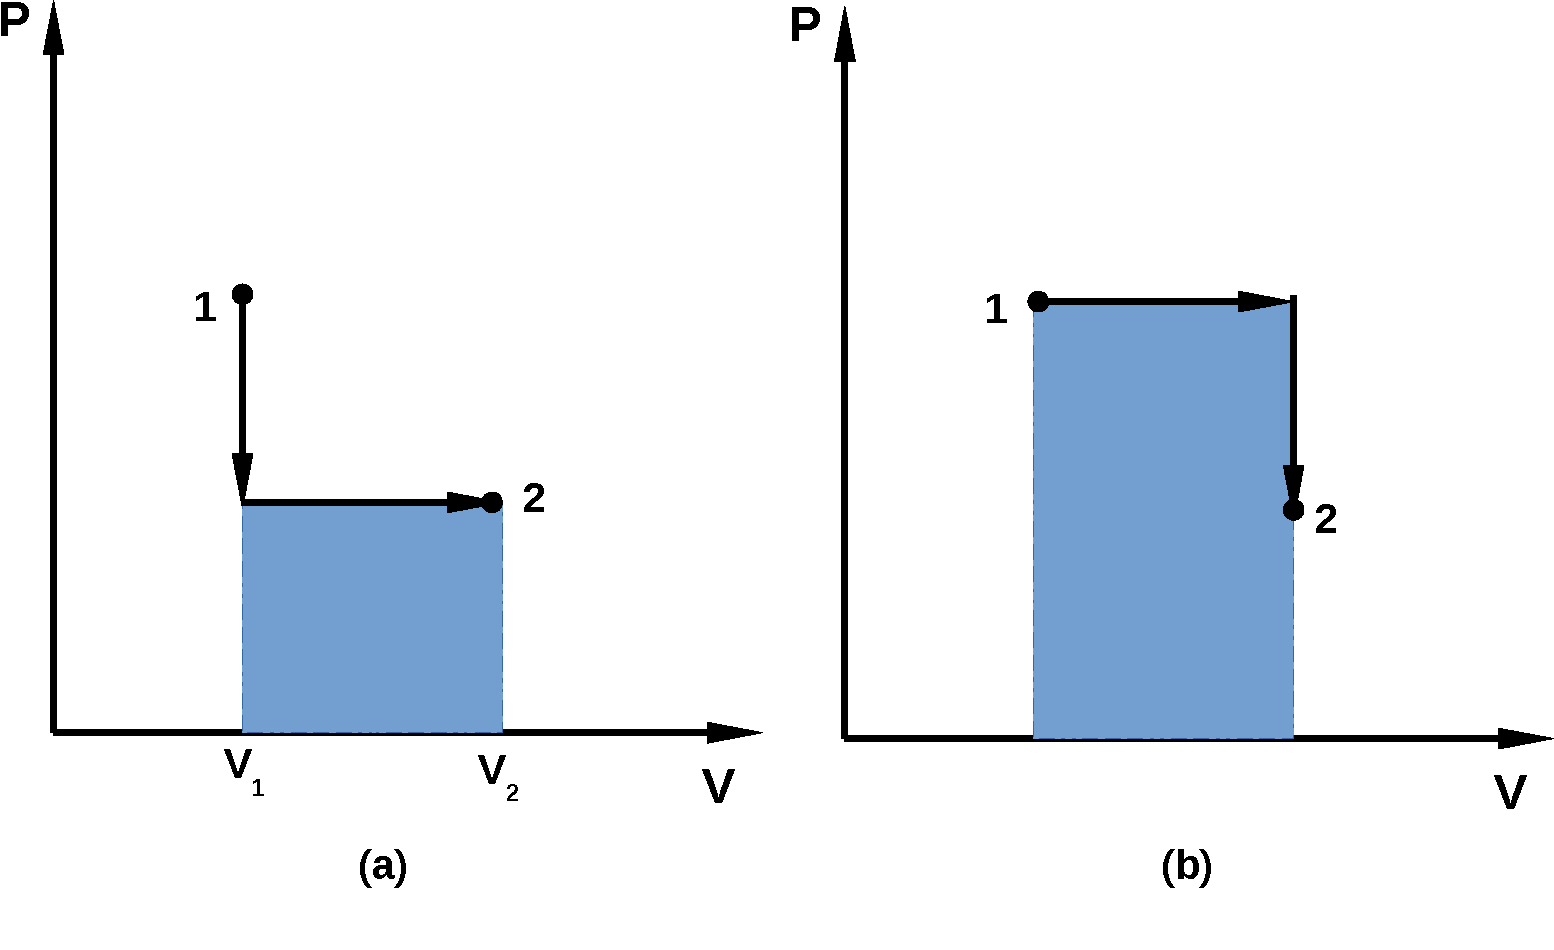
\includegraphics[width=.6\columnwidth,clip]{./Figs/Mod1Ex1}
           \vspace{-.1cm}\caption{Expansion processes (Example~\ref{Mod01Ex01}).}\label{Mod01Fig01}
         \end{center}
       \end{figure}

% SOLUTION
       \noindent{\bf Solution:} $W_{\text{rev}}$ is related to the area below the curve. Thus, we should use the $PV$ work equation:
           \begin{itemize}
              \item For process {\bf (a)}: 
                 \begin{eqnarray}
                    d W = -PdV \Longrightarrow W &=& -P_{2}\left(V_{2}-V_{1}\right) \nonumber \\
                                                 &=& - 1\text{ atm}\left(2000-500\right)\text{ cm}^{3} = -1500\text{ atm.cm}^{3} \nonumber 
                 \end{eqnarray}
                 Now we need to convert {\it atm.cm}$^{3}$ to $J$, thus using the unit conversion table:
                 \begin{eqnarray}
                     W &=& -1500\blue{\cancel{\text{ atm}}}.\red{\cancel{\text{cm}^{3}}} \frc{1.01325\times 10^{5}\blue{\cancel{\text{ Pa}}}}{1\blue{\cancel{\text{ atm}}}} \frc{1 \frc{\text{kg}}{\text{m.s}^{2}}}{1\blue{\cancel{\text{ Pa}}}} \frc{1\text{ m}^{3}}{ 100^{3} \red{\cancel{\text{ cm}^{3}}}} \nonumber \\
                       &=& -151.9875 \blue{\cancel{\frc{\text{ kg.m}^{2}}{\text{s}^{2}}}} \frc{ 1 \text{ J}}{ \blue{\cancel{\frc{\text{ kg.m}^{2}}{\text{s}^{2}}}}} \nonumber\\
                       &=& -151.9875\text{ J} \nonumber
                 \end{eqnarray}
%
              \item For process {\bf (b)}, since $P$ is constant, i.e., $P_{1}=P_{2}$:
                 \begin{eqnarray}
                    d W = -PdV \Longrightarrow W &=& -P_{1}\left(V_{2}-V_{1}\right) \nonumber \\
                                                 &=& - 3\text{ atm}\left(2000-500\right)\text{ cm}^{3} = -4500\text{ atm.cm}^{3} \nonumber \\
                                                 &=& -455.9625\text{ J} \nonumber
                 \end{eqnarray}
           \end{itemize}
\clearpage

%%%
%%% EXAMPLE
%%%
   \item Calculate the internal energy (in $J$) when 1 mol of water is isobarically heated from 25$^{\circ}$C to 30$^{\circ}$C at 1 atm. Given: densities of water are 0.9970 g.cm$^{-3}$ at 0$^{\circ}$C and 0.9956 g.cm$^{-3}$ at 100$^{\circ}$C. Molar mass and heat capacity at constant pressure of water are 18 g.mol$^{-1}$ and 1 cal.$\left(\text{g.}^{\circ}\text{C}\right)^{-1}$, respectively.

% SOLUTION
       \noindent{\bf Solution:} From the 1$^{\text{st}}$ Law, $U=Q+W$ ,and in order to calculate $U$ we first need to obtain heat ($Q$) and work ($W$). $Q$ can be obtained from the heat capacity equation
          \begin{displaymath}
             Q = m C_{p} \Delta T,
          \end{displaymath}  
          where $m$ is the mass of water can be obtained from
          \begin{displaymath}
             n = \frc{m}{MW} \Longrightarrow  m = n.MW = 1\text{ mol} . 18 \frc{\text{g}}{\text{mol}} = 18 \text{ g}
          \end{displaymath}
          $n$ and $MW$ are number of moles and molar mass, respectively. Now,
          \begin{displaymath}
             Q = m C_{p} \Delta T = 18\text{ g} . 1 \frc{\text{ cal}}{\text{g.}^{\circ}\text{C}}.\left(30-25\right)^{\circ}\text{C} = 90\text{ cal}
          \end{displaymath}  
          Now, we should calculate the work through $W=-P\Delta V$, however $V$ is not known, but we can obtain it from the density relation $V=m/\rho$, thus
          \begin{displaymath}
             W = - P\Delta V = -P\left(V_{2}-V_{1}\right) = -P\left(\frc{m}{\rho_{2}} - \frc{m}{\rho_{1}}\right) = -0.025\text{atm.cm}^{3} = -0.0006\text{ cal} 
          \end{displaymath}
          Now, calculating the internal energy,
          \begin{displaymath}
             U = Q + W = 89.9994\cancel{\text{ cal}} . \frc{ 4.186\text{ J}}{1\cancel{\text{ cal}}} = 376.7375 \text{ J}
          \end{displaymath}

\clearpage
%%%
%%% EXAMPLE
%%%
   \item A 0.3 m$^{3}$  tank contains oxygen initially at 100 kPa and 300 K. A paddle wheel within the tank is rotated until the pressure inside rise to 150 kPa. During the process 2 kJ of heat is lost to the surroundings. Determine the paddle-wheel work done (in kJ). Neglect the energy stored in the paddle wheel and assume the heat capacity at constant volume of oxygen is 0.6745 kJ.$\left(\text{kg.K}\right)^{1}$. Given molar mass of oxygen of 32 g.mol$^{-1}$.

% SOLUTION
       \noindent{\bf Solution:} The volume of the tank remains constant $V_{2}=V_{1}=V=$ 0.3 m$^{3}$ during the whole process. Thus, we can define:
            \begin{center}
              \begin{tabular}{l l l l}
                 Initial Condition & $P_{1}=$ 100 kPa   & $T_{1}=$ 300 K         & $V_{1}=$ 0.3 m$^{3}$  \\
                 Final Condition   & $P_{2}=$ 150 kPa   &                       & $V_{2}=$ 0.3 m$^{3}$ \\
                 Heat Loss         & $Q=$ -2 kJ        &                       &                    
              \end{tabular}
            \end{center}
       The compression occurs in a closed system (i.e., constant mass) and, as there is no further information, we may consider that oxygen behaves as an ideal gas. The work added to the system by the paddle can be expressed by $U=Q+W$. Our first step is to calculate $T_{2}$,
       \begin{displaymath}
          \frc{P V}{T} = \text{ constant} \Rightarrow \frc{P_{1}V_{1}}{T_{1}} = \frc{P_{2}V_{2}}{T_{2}} \Rightarrow \frc{P_{1}}{T_{1}}=\frc{P_{2}}{T_{2}} \Rightarrow T_{2} = 450\text{ K}
       \end{displaymath}
        The specific internal energy can defined by the fundamental relation, $du=C_{v}dT$ (check the units for this relation!), where $C_{v}$ is the heat capacity at constant volume thus,
       \begin{displaymath}
          \Delta U = m\Delta u = C_{v}\Delta T = Q + W,
       \end{displaymath}
       therefore, we need to obtain the mass of oxygen in the tank through the ideal gas equation of state,
       \begin{eqnarray}
         P V = n R T \Rightarrow n = \frc{m}{MW} = \frc{P V}{R T} \Rightarrow m &=& \frc{ MW P V}{R T} \nonumber \\
                                                      &=& \frc{ 32\frc{\text{ g}}{\text{mol}} 100\text{ kPa} . 0.3\text{ m}^{3}}{ 8.3143 \frc{\text{J}}{\text{mol.K}} 300\text{ K}} \nonumber \\
                                                      &=& 0.3848 \frc{\text{ g.kPa.m}^{3}}{\text{J}} \frc{1 \text{ J}}{1\text{ N.m}} \frc{1000 \text{ Pa}}{1 \text{ kPa}} \frc{ 1 \text{ N.m}^{-2}}{1\text{ Pa}} \nonumber\\
                                                      &=& 0.3848\text{ kg}\nonumber
       \end{eqnarray}
       Thus
       \begin{eqnarray}
          \Delta u = m C_{v}\Delta T = Q + W \Rightarrow W &=& m C_{v}\left(T_{2}-T_{1}\right) - Q \nonumber \\
                                                          &=& 0.3848\text{ kg} \times 0.6745 \frc{\text{kJ}}{\text{kg.K}}\times (450-300)\text{ K} - (-2 \text{ kJ}) \nonumber \\
                                                          &=& 40.9321\text{ kJ}. \nonumber
       \end{eqnarray}
       The paddle-wheel executed 40.9321 kJ of work to the system.

\clearpage
%%%
%%% EXAMPLE
%%%
   \item  Air initially occupying 1 m$^{3}$ at 1.5 bar and 20$^{\circ}$C undergoes an internally reversible compression for which $P V^{\gamma}=$ constant to a final state where the pressure is 6 bar and the temperature is 120$^{\circ}$C. Determine:
        \begin{enumerate}[(a)]
           \item Value of $\gamma$;
           \item Work and the heat transfer (in kJ).
       \end{enumerate}
       Assume that heat capacity at constant volume and molar mass of air are 0.718 kJ.$\left(\text{kg.K}\right)^{-1}$ and 29 g.mol$^{-1}$. 

% SOLUTION
       \noindent{\bf Solution:}
        \begin{center}
           \begin{tabular}{c c c c}
               {\bf State}  &   $P$ (atm)  &   $T\;\left(^{\circ}\text{C}\right)$ & $V\;\left(\text{m}^{3}\right)$ \\
                    1       &     1.5      &            20                      & 1  \\
                    2       &     6.0      &            120                     &     \\              
           \end{tabular}
        \end{center}
        \begin{enumerate}[(a)]
           \item In order to calculate the isentropic index $\gamma$, we can use any of the relations learned in the lecture,
               \begin{displaymath} 
                   P V^{\gamma} = C, \hspace{1cm} T V^{\gamma-1} = C \hspace{1cm} \text{ and/or } \hspace{1cm} T P^{\frac{1-\gamma}{\gamma}} = C.
               \end{displaymath}
               Although $P$ and $V$ is the relation initially given in the problem, we do not know the final volume of air, $V_{2}$. However, initial and final pressure and temperature are known and we can make use of this relationship to obtain $\gamma$,
               \begin{eqnarray} 
                   T P^{\frac{1-\gamma}{\gamma}} = C \Rightarrow T_{1}P_{1}^{\frac{1-\gamma}{\gamma}} = T_{2}P_{2}^{\frac{1-\gamma}{\gamma}} \nonumber \\
                   \left(\frc{P_{1}}{P_{2}}\right)^{\frac{1-\gamma}{\gamma}} = \frc{T_{2}}{T_{1}} \Rightarrow \frc{1-\gamma}{\gamma} = \frc{\ln{\frac{T_{2}}{T_{1}}}}{\ln{\frac{P_{1}}{P_{2}}}} \Longrightarrow \gamma = 1.2686  \nonumber
               \end{eqnarray}
                 
           \item Compression work can be obtained by integrating $\d W = -P dV$ from state 1 to state 2 with $P=\frac{C}{V^{\gamma}}$,
               \begin{eqnarray}
                 W_{1-2} &=& -\int\limits_{V_{1}}^{V_{2}} P dV = -\int\limits_{V_{1}}^{V_{2}}\frc{C}{V^{\gamma}} dV = -\left.\frc{C}{1-\gamma}V^{1-\gamma}\right|_{V_{1}}^{V_{2}} \nonumber \\
                         &=& -\frc{C}{1-\gamma}\left(V_{2}^{1-\gamma}-V_{1}^{1-\gamma}\right),\;\;\text{ however, as } C=P_{1}V_{1}^{\gamma}=P_{2}V_{2}^{\gamma} \nonumber \\
                         &=& -\frc{P_{2}V_{2}^{\gamma}V_{2}^{1-\gamma} - P_{1}V_{1}^{\gamma}V_{1}^{1-\gamma}}{1-\gamma} = \frc{P_{1}V_{1}-P_{2}V_{2}}{1-\gamma} \nonumber
               \end{eqnarray}
               The relation above, although important, can not be used as we do not know $V_{2}$, however we can change variables through the ideal gas relation
               \begin{eqnarray}
                  P V = n R T &\Rightarrow& n = \frc{P V}{R T } = \frc{1.5\text{ atm} \times 1\text{ m}^{3}}{ 8.3143 \frc{\text{J}}{\text{mol.K}} 293.15\text{ K}} \frc{1.01325\times 10^{5} \text{ Pa}}{1 \text{ atm}} \frc{ 1 \text{ N.m}^{-2}}{1\text{ Pa}}\frc{1 \text{ J}}{1\text{ N.m}} = 62.3580\text{ moles}\nonumber \\
                   % m &=& \frc{P_{1} V_{1} MW}{R T_{1}} = \frc{1.5\text{ atm} \times 1\text{ m}^{3} \times 29 \frac{\text{g}}{\text{mol}} } { 8.3143 \frc{\text{J}}{\text{mol.K}} 293.15\text{ K}} \frc{1 \text{ J}}{1\text{ N.m}} \frc{1.01325\times 10^{5} \text{ Pa}}{1 \text{ atm}} \frc{ 1 \text{ N.m}^{-2}}{1\text{ Pa}} = 1808.38 \text{ g}\nonumber\\
                    W &=& \frc{P_{1}V_{1}-P_{2}V_{2}}{1-\gamma} = nR\frc{T_{1}- T_{2}}{1-\gamma} \nonumber \\
                      &=& 62.3580\text{ mol} \times 8.3143 \frc{\text{J}}{\text{mol.K}} \times \frc{\left(293.15-393.15\right)\text{ K}}{1-1.2686} \nonumber \\
                      &=& 193024.2440 \text{ J} \Longrightarrow W = -193.02 \text{ kJ} \nonumber
               \end{eqnarray}
              Heat ($Q$) can be obtained from
               \begin{eqnarray}
          \Delta u &=& m C_{v}\Delta T = n MW C_{v}\Delta T = Q + W  \nonumber \\
             Q &=& n MW C_{v}\left(T_{2}-T_{1}\right) - W \nonumber \\
               &=& 62.3580\text{ mol}\times 29 \frc{\text{g}}{\text{mol}} \red{\frc{1\text{ kg}}{1000\text{ g}}}\times 0.718\frc{\text{kJ}}{\text{kg.K}}\times (393.15-293.15)\text{ K} - 193.30 \text{ kJ} \nonumber \\
                                                          &=& -63.46\text{ kJ}. \nonumber                   
               \end{eqnarray}
       \end{enumerate}


\clearpage
%%%
%%% EXAMPLE
%%%
   \item Two kg of water at 80$^{\circ}$C is mixed adiabatically with 3 kg of water at 30$^{\circ}$C in a constant pressure process of 1 atm. Find the increase in entropy $\left(\text{in kJ.K}^{-1}\right)$ of the total mass of water due to the mixing process. Assume that $C_{p}$ of water is 4.187 kJ.$\left(\text{kg.K}\right)^{-1}$. 

% SOLUTION
       \noindent{\bf Solution:} From the classic thermodynamic definition of reversible entropy processes (second law),
         \begin{displaymath}
            d S = \frc{d Q}{T}
         \end{displaymath}
         with $dQ = m C_{p}dT$, then integrating 
         \begin{eqnarray}
            \int\limits_{S_{i}}^{S_{f}} dS &=& m C_{p}\int\limits_{T_{i}}^{T_{f}}\frc{dT}{T} \nonumber \\
            \Delta S &=& S_{f}-S_{i} = m C_{p} \ln{\frc{T_{f}}{T_{i}}} \nonumber
         \end{eqnarray}
         Assuming that the system is adiabatic, we can calculate the final temperature $\left(T_{f}\right)$ from thermal energy conservation principles: 
         \begin{displaymath}
            m_{1}C_{p,1}T_{1} + m_{2}C_{p,2}T_{2} = \left(m_{1}+m_{2}\right)C_{p}T_{f} \rightarrow T_{f} = 50^{\circ}\text{C} = 323.15\text{ K}
         \end{displaymath}
         And the entropies are
         \begin{eqnarray}
             \Delta S_{1} &=& m_{1}C_{p,1}\ln{\frc{T_{f}}{T_{1}}} =  -0.7434\frc{\text{kJ}}{\text{K}} \nonumber \\
             \Delta S_{2} &=& m_{2}C_{p,2}\ln{\frc{T_{f}}{T_{2}}} =  0.8025\frc{\text{kJ}}{\text{K}} \nonumber 
         \end{eqnarray}
         Thus the increase in entropy of the total mass is
         \begin{displaymath}
              \Delta S_{\text{mix}} = \Delta S_{1} + \Delta S_{2} = 0.0591\frc{\text{kJ}}{\text{K}}
         \end{displaymath}
%
\end{enumerate}

\clearpage
%%%%%%%%%%%%%%%%%%%%%%%%%%%%%%%%%%%%%%%%%%%%%%%%%%%%%%%%%%%%%%%%%%%%%%%%%%%%%%%%%%%%%%%%%%%%%%%%%%%%%%%%%%%%%%%%%%%%%%%%%%%%%%%%%%%%%%%%%%%%%%
%%%%%%%%%%%%%                                                    END OF MODULE 01                                                %%%%%%%%%%%%%
%%%%%%%%%%%%%%%%%%%%%%%%%%%%%%%%%%%%%%%%%%%%%%%%%%%%%%%%%%%%%%%%%%%%%%%%%%%%%%%%%%%%%%%%%%%%%%%%%%%%%%%%%%%%%%%%%%%%%%%%%%%%%%%%%%%%%%%%%%%%%%

%%%
%%% SECTION 2
%%%
\section{Module 02: Volumetric Properties of Pure Fluids}\label{Section:02}


%%% SUBSECTION
\subsection{PVT Behaviour of Pure Substances}\label{Section:02:PVTBehaviour}
  
   \begin{enumerate}[i)]
%
       \item {\it Pure substances/fluids} can be defined as a material of homogeneous and constant composition. Systems containing (a) water and ice, (b) water and steam or (c) water, ice and steam are examples of pure fluids at different phases, whereas (d) air-water, (e) air-steam and (f) a gaseous mixture containing N$_{2}$, H$_{2}$, O$_{2}$ and NO$_{2}$ are not. 
%
       \item A pure fluid can exist and coexist in different phases (\ie solid, liquid and vapour -- S, L and V). Phase behaviour of fluids is often represented by {\it PVT}\footnote{{\it PVT} stands for pressure, specific (or molar) volume and temperature.} phase diagrams. 
%
       \item {\it PVT} diagram of an arbitrary fluid is shown as 3D representation in Figure~\ref{Mod02Fig01}a. Solid, liquid and vapour phases are represented by continuous volumes and, the regions between these volumes are representations of \blue{phase equilibrium}.
%
           \begin{figure}[h]
              \begin{center}
                 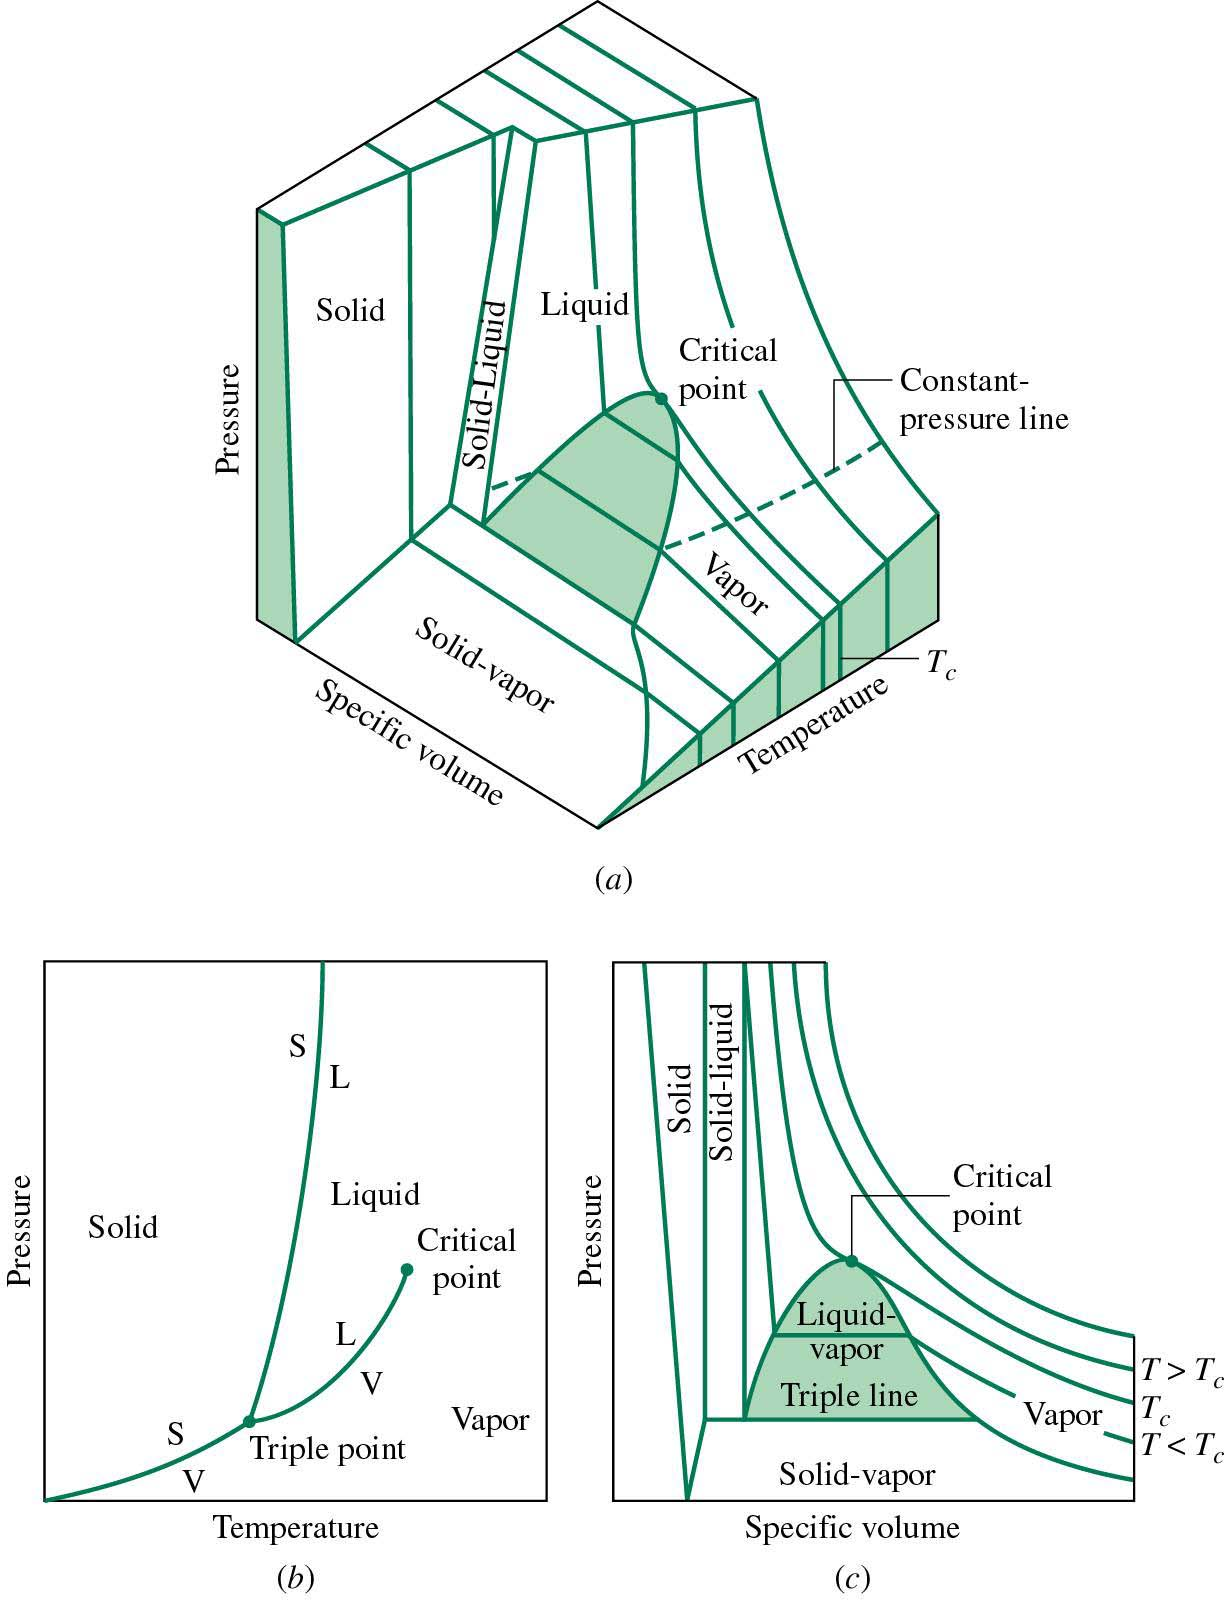
\includegraphics[width=10.cm,clip]{./../Pics/PVT_Surface.jpg}\label{Mod02Fig01}
                 \caption{$PVT$ volume (top) and projections onto (b) $PT$ and (c) $PV$ diagrams for a pure substance (Extracted from Borgnakke $\&$ Sonntag).}\label{Mod02Fig01}
              \end{center}
           \end{figure}    
%
       \item Such 3D representation helps determining (qualitatively) phases (S, L and V) at prescribed coordinates (temperature, specific/molar volume and pressure) of fluids. However, it is not convenient dealing with 3D plots and, most of the time, we may want to extract quantitative values of fluids (Module 03). A better approach is to project 3D plots into surfaces, \ie $PT$, $PV$ and $VT$ diagrams (Figs.~\ref{Mod02Fig01}b and~\ref{Mod02Fig01}c).
%
       \item $PV$ diagrams (Fig.~\ref{Mod02Fig02}a) are representations of Fig.~\ref{Mod02Fig01}a at constant specific temperature, where surfaces represent both single phases and phase transitions (\ie phases in equilibrium). Here, there are three properties that we need to define:
           \begin{enumerate}[a)]
              \item Critical point (or state): coordinates in which two phases of a fluid become indistinguishable. Beyond this coordinate, a fluid is neither completely liquid nor completely gaseous, \ie exhibits properties of both the liquid phase and the gas phase and is referred to as a {\it supercritical fluid}. All fluids have distinct critical coordinates, known as {\it critical pressure} $\left(\text{P}_{c}\right)$, {\it critical temperature} $\left(\text{T}_{c}\right)$ and {\it critical volume} $\left(\text{V}_{c}\right)$. Interesting videos about critical state can be seen in \href{https://www.youtube.com/watch?v=bJjcTpRzXpM}{https://www.youtube.com/watch?v=bJjcTpRzXpM} and \href{https://www.youtube.com/watch?v=RmaJVxafesU}{https://www.youtube.com/watch?v=RmaJVxafesU}.
              \item Saturation lines (blue lines in Fig.~\ref{Mod02Fig02}a) are coordinates in which phase transition starts to occur.
              \item Isotherms: Lines of constant temperature.
           \end{enumerate} 
           In vapour-liquid equilibrium (VLE) systems there are two main saturation lines: {\it saturated liquid line} (left-hand side of $C$ in Fig.~\ref{Mod02Fig02}a)  and {\it saturated vapour line} (rhs of $C$) that represent the initial transition from a single phase system to a two or three phases system. 
%
       \item $PT$ diagrams (Fig.~\ref{Mod02Fig02}b) are representations of Fig.~\ref{Mod02Fig01}a at constant specific volumes, where phases are defined by surfaces with continuous lines representing phases transitions (\ie in equilibrium). The {\it triple point} is coordinate in which all three phases (S, L and V) coexist in equilibrium.
%
           \begin{figure}[h]\label{Mod02Fig02}
              \vbox{
                    \hbox{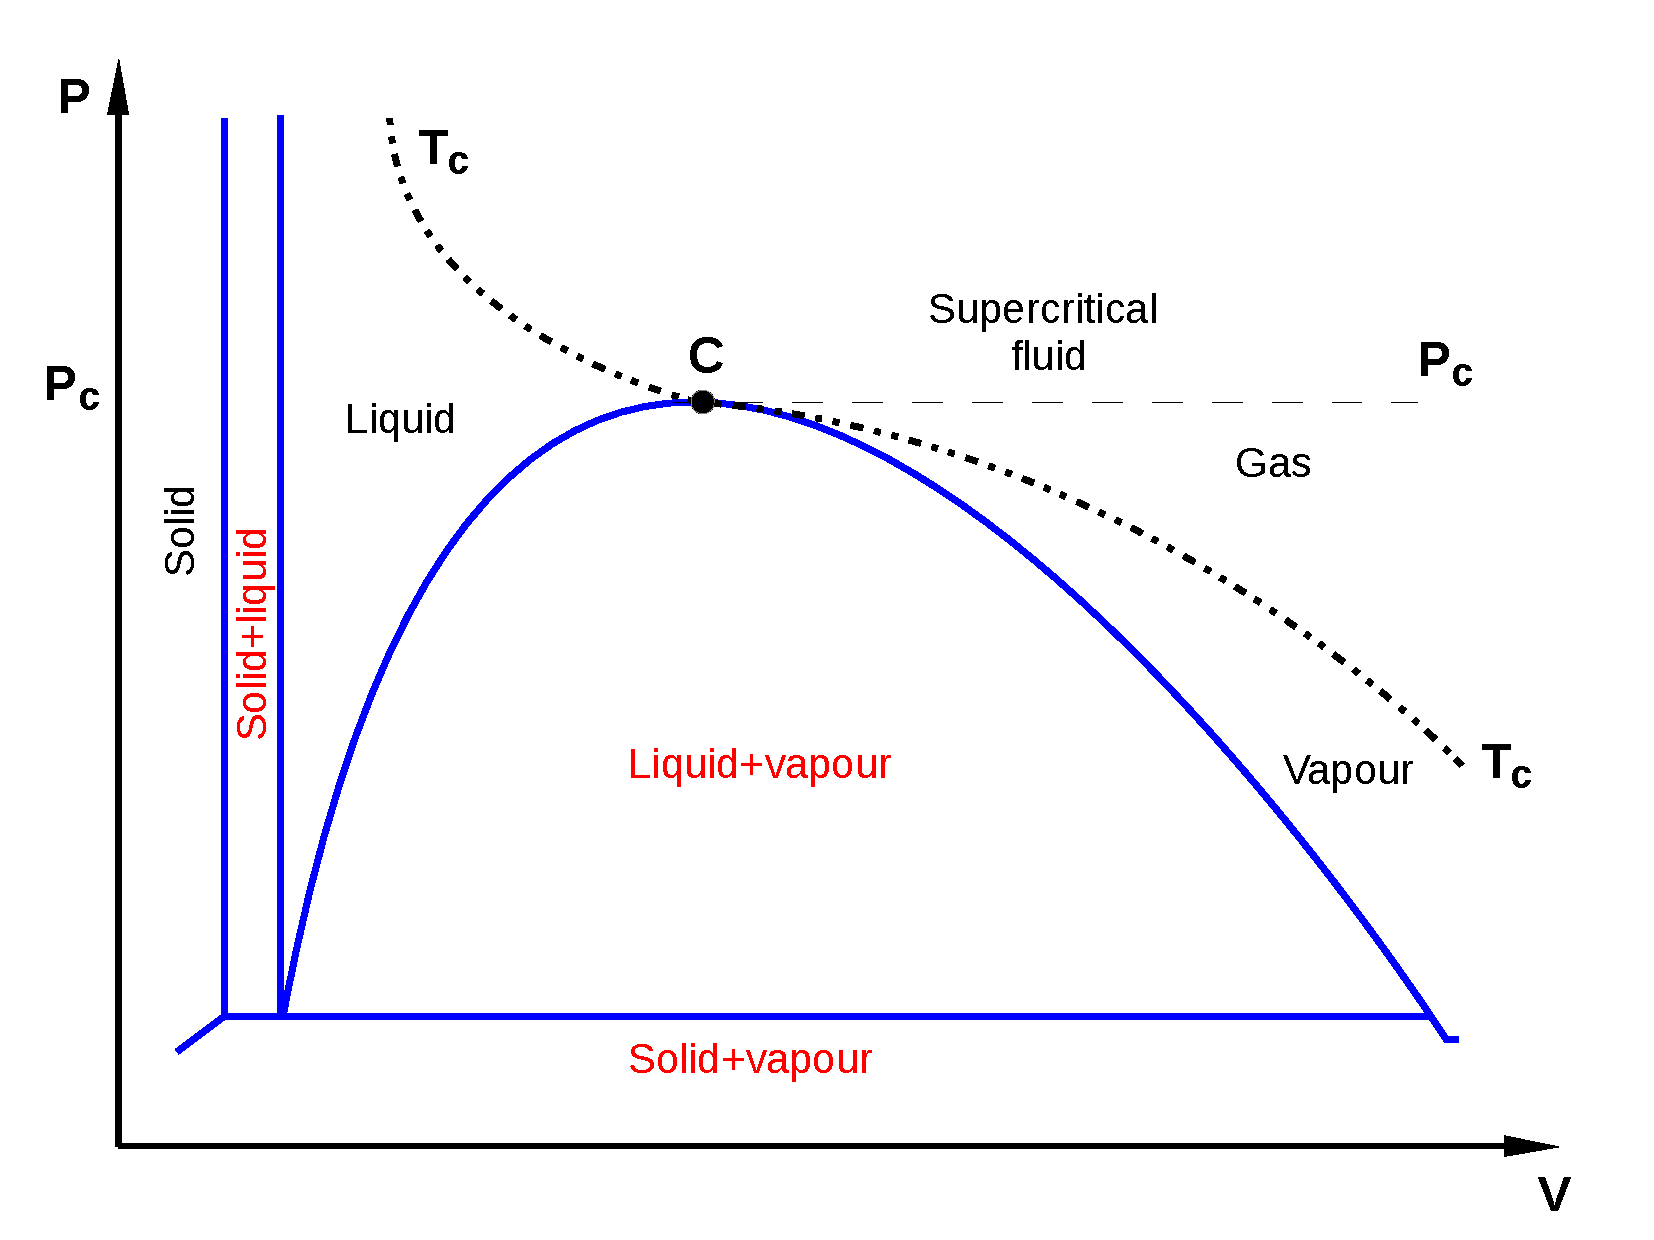
\includegraphics[width=.5\columnwidth,clip]{./../Pics/PV_Diagram1}
                          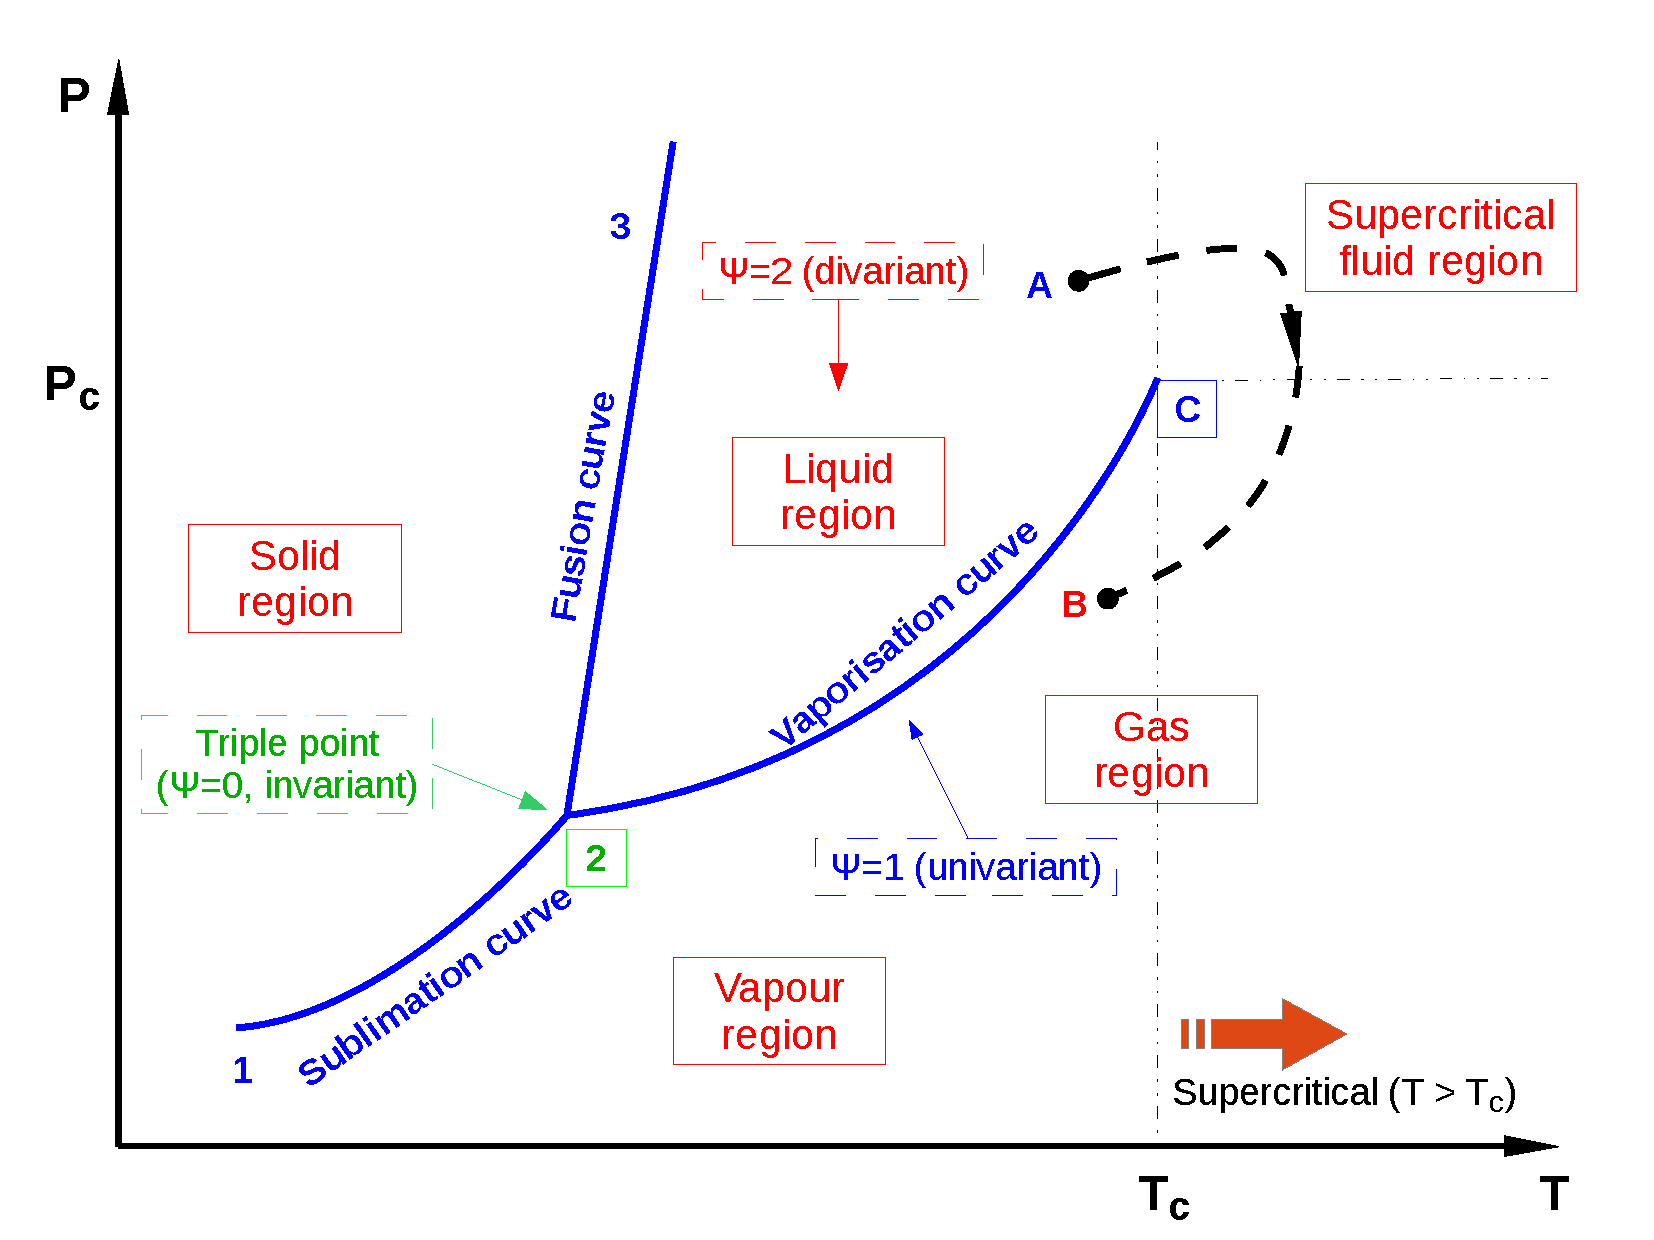
\includegraphics[width=.5\columnwidth,clip]{./../Pics/PT_Diagram}}
                    \vspace{-.1cm}
                    \hbox{\hspace{4cm}(a)\hspace{8cm}(b)}}
              \caption{ (a) $PV$ and (b) $PT$ diagrams for a pure substance. Dotted line in (a) represents the isotherm at T=T$_{c}$.}\label{Mod02Fig02}
           \end{figure}
%
        \item A fluid in the compressed liquid state is often called {\it sub-cooled fluid} (central region of Fig.~\ref{Mod02Fig02}b), while a gas at a pressure lower than its saturation vapour pressure for a given temperature is said to be at {\it superheated state}.
%
        \item The \underline{Gibbs phase rule} is a relation that determines the number of independent variables that must be specified to establish the {\it intensive state of any system at equilibrium},
                \begin{equation}
                    \Psi = 2 + \mathcal{C} - \mathcal{P} -\mathcal{R},\label{Mod02_GibbsPhaseRuleReactive}
                \end{equation}
                where $\Psi$, $\mathcal{C}$, $\mathcal{P}$ and $\mathcal{R}$ are the number of degrees of freedom of the thermodynamic system, number of chemical components, number of co-existing phases and number of independent reactions, respectively. For non-reactive systems\footnote{The Gibbs phase rule will be revisited again in Module~\ref{Section:06} -- Chemical Reaction Equilibrium.}, this relation becomes,
                \begin{equation}
                    \Psi = 2 + \mathcal{C} - \mathcal{P}.\label{Mod02_GibbsPhaseRule}
                \end{equation}
                The degrees of freedom ($\Psi$, \ie number of intensive properties such as temperature and pressure) determines the number of variables that must be specified to fix all other remaining phase rule variables. For example, for a pure liquid component, the phase rule yields two degrees of freedom, \ie if temperature and pressure are specified, all other intensive properties (\eg enthalpy, entropy etc) are uniquely determined. However, if the same liquid component is in equilibrium with its vapour phase (\eg water and steam) there is {\it only} one degree of freedom. This means that either pressure or temperature may be specified to fix all other intensive properties of the system. At the triple point (\eg water, steam and ice), the number of degrees of freedom is {\it zero}, \ie any change from such state (\eg for water-steam-ice at $\sim$ 273.15 K and 0.0061 bar) causes at least one of the phases to vanish.
%
        \item The ideal gas {\it equation of state} (EOS),
                \begin{equation}
                   P V = R T,\label{Mod02_IdealEOS}
                \end{equation}
                where $V$ is the molar volume. This is a relationship between the macroscopic intensive properties, and is based in two main assumptions with respect to the microscopic behaviour of molecules:
            \begin{enumerate}[(a)]
                \item Molecules have no extension in space (\ie zero volume), and;
                \item Molecules \underline{do not interact with each other}.
            \end{enumerate}
            The second assumption is particularly important as it considers that atoms and molecules either do not interact or do not have electric charge or have an infinite distance between them (\ie low density conditions).
%
        \item However, these assumptions are rarely met in real conditions (both in the environment and in industry) and several mathematical relations have been developed to better represent the PVT behaviour of real fluids:
            \begin{enumerate}[a)]
%
                \item The PVT behaviour of real pure fluids can be expressed as functional $f(P,V,T) = 0$. However, from the Gibbs phase rule for a single phase pure component the number of degrees of freedom is equal to 2. Therefore, we can write this function in its simplest way (or EOS), $V=V(T,P)$, or in differential form,
                   \begin{displaymath}
                      dV = \left(\frc{\partial V}{\partial T}\right)_{P}dT + \left(\frc{\partial V}{\partial P}\right)_{T}dP
                   \end{displaymath}
                   defining the {\it coefficient of thermal expansion} (or {\it volume expansivity coefficient}), $\beta$, and the {\it coefficient of isothermal compressibility}, $\kappa$ as,
                   \begin{equation}
                      \beta \equiv \frc{1}{V}\left(\frc{\partial V}{\partial T}\right)_{P}\;\;\;\text{ and }\;\;\;\kappa \equiv -\frc{1}{V}\left(\frc{\partial V}{\partial P}\right)_{T},\label{Mod02_Compressibilityexpansivity}
                   \end{equation}
                   respectively, leading to
                   \begin{equation}
                       \frc{dV}{V} = \beta dT - \kappa dP.\label{Mod02_Compressibilityexpansivity2}
                   \end{equation}
%
                \item The {\it Virial EOS} is a relation that can be derived from statistical mechanics, and is represented by power series in terms of $\frac{1}{V}$ with two alternate forms:
                   \begin{eqnarray}
                       \frc{P V}{R T} &=& 1 + \frc{B}{V} + \frc{C}{V^{2}} + \cdots \text{ or} \label{Mod02_Virial1}\\
                       \frc{P V}{R T} &=& 1 + B^{\prime}P + C^{\prime}P^{2} + \cdots,\label{Mod02_Virial2} 
                   \end{eqnarray}
                   where $B$ and $C$ are the second and third virial coefficients and,
                   \begin{displaymath}
                      B = \frc{B^{\prime}}{R T}\;\;\;\text{ and }\;\;\; C^{\prime}=\frc{C-B^{2}}{\left(R T\right)^{2}}.
                   \end{displaymath}
                   Second and third terms of Eqns.~\ref{Mod02_Virial1} and~\ref{Mod02_Virial2} are \blue{corrections of the non-ideal behaviour of a gas}. Virial coefficients are strongly dependent on the temperature (\ie $B=B(T)$, $C=C(T)$, $D=D(T)$ etc) and the more the number of coefficients (\ie the more terms in the power series -- Eqns.~\ref{Mod02_Virial1} and~\ref{Mod02_Virial2}) the better is the predictions of the gas molar volume. The second virial coefficient is readily found for a large number of fluids in any chemical engineering handbook (and several textbooks), however the third and further coefficients are more difficult to obtain/calculate. Therefore the Virial EOS is often used for moderate deviations from the ideal gas behaviour through the truncated forms of Eqns.~\ref{Mod02_Virial1} and~\ref{Mod02_Virial2}
                   \begin{eqnarray}
                      \frc{P V}{R T} &=& 1 + \frc{B}{V} \;\;\;\;\text{ or } \label{Mod02_Virial1b}\\
                      Z &=& 1 + \frc{B P}{R T} = 1 + \frc{B P_{c}}{R T_{c}}\frc{P_{r}}{T_{r}},\label{Mod02_Virial1c}
                   \end{eqnarray}
                   where,
                   \begin{equation}
                      T_{r} = \frc{T}{T_{c}}\;\;\;\;\text{ and }\;\;\;\; P_{r} = \frc{P}{P_{c}}\label{Mod02_ReducedT-P},
                   \end{equation}
                   are {\it reduced temperature and pressure}, respectively. $Z = \frac{P V}{R T}$ is the \underline{compressibility factor} and can be defined as the ratio of the molar volume of a gas to the molar volume of an ideal gas at the same temperature and pressure conditions -- for an ideal gas, $Z=1$. 

                   A number of {\it generalised relations} have been developed to calculate the {\it second virial coefficients}, \eg
                   \begin{displaymath}
                      \frc{B P_{c}}{R T_{c}} = B^{0} + \omega B^{1},
                   \end{displaymath}
                   with terms $B^{0}$ and $B^{1}$ defined by,
                   \begin{displaymath}
                      B^{0} = 0.083 - \frc{0.422}{T_{r}^{1.6}}\;\;\text{ and }\;\; B^{1} = 0.139 - \frc{0.172}{T_{r}^{4.2}}.
                   \end{displaymath}
                   $\omega$ is a parameter known as \underline{acentric factor} that measures the non-sphericity of molecules,
                   \begin{displaymath}
                      \omega \equiv -1 - \log\limits_{10}{\left(P_{r}^{\text{sat}}\right)_{T_{r}=0.7}},
                   \end{displaymath}
                   where $\left(P_{r}^{\text{sat}}\right)_{T_{r}=0.7}$ is the reduced saturation vapour pressure obtained at reduced temperature of 0.7. Tabulated acentric factor for a number of chemical species can be found in any thermodynamic textbook.
%
                \item The truncated form of the {\it Virial EOS} can be used to represent PVT behaviour of gases with reasonable accuracy at relatively low pressures. At moderate and high pressures, predicted volumetric properties deviate from expected and alternative EOS formulations have been developed. \underline{Cubic EOS} are widely used in \blue{flow and process simulators} to represent PVT behaviour of fluids, and were developed as a cubic function of the molar volume (or the compressibility factor, $Z$). Cubic equations of state can result in (reasonable) accurate prediction of both gas and liquid (saturated) molar volumes and are relatively easy to implement. Since the development of the first cubic EOS in the 19$^{\text{th}}$ century, several EOS have been proposed and used by industry. Four of the most important cubic EOS are listed below:
                   \begin{enumerate}[c.1)]
%
                      \item The \underline{van der Walls} (vdW) EOS was originally developed in 1873 and has the form,
                          \begin{equation}
                             P = \frc{R T}{V-b} - \frc{a}{V^{2}},\label{Mod02_vdWEOS}
                          \end{equation}
                          where $a$ is called the {\it attraction parameter} and $b$ is the {\it repulsive parameter} (or {\it effective molecular volume} or {\it co-volume}), 
                          \begin{displaymath}
                              a = \frc{27}{64}\frc{R^{2}T_{c}^{2}}{P_{c}},\;\;\; b = \frc{1}{8}\frc{R T_{c}}{P_{c}},
                          \end{displaymath}
                          and they take into account interactions between molecules. Although this EOS is able to predict volumetric properties of gasses better than the ideal EOS, it is still very inaccurate for liquids and for fluids at high pressure.  Redlich-Kwong and Soave-Redlich-Kwong EOS were formulated in the 40's and 70's and became increasingly popular in the oil $\&$ gas and petrochemical sectors. 
%
                      \item Redlich-Kwong (RK EOS):
                           \begin{equation}
                               P = \frc{R T}{V-b} - \frc{a}{V\sqrt{T}\left(V+b\right)},\label{Mod02_RKEOS}
                           \end{equation}
                           with,
                          \begin{displaymath}
                              a = \frc{0.42748 R^{2}T_{c}^{2}}{P_{c}},\; \text{ and }\;\;\; b = \frc{0.08664 R T_{c} }{P_{c}}.
                          \end{displaymath}
%
                      \item Soave-Redlich-Kwong (SRK EOS):
                           \begin{equation}
                               P = \frc{R T}{V-b} - \frc{a\alpha}{V\left(V+b\right)},\label{Mod02_SRKEOS}
                           \end{equation}
                           with,
                          \begin{eqnarray}
                              &&a = \frc{0.427 R^{2}T_{c}^{2}}{P_{c}},\;\;\;b = \frc{0.08664 R T_{c} }{P_{c}} \nonumber \\
                              &&\text{and }\;\;\; \alpha = \left[1 + \left( 0.48508 + 1.55171\omega - 0.15613\omega^{2}\right)\left(1-\sqrt{T_{r}}\right)\right]^{2}\nonumber
                          \end{eqnarray}                          
%
                      \item Peng-Robinson (PR EOS): it is by far the most used EOS used in simulators and is able to predict molar volume with good accuracy,
                           \begin{equation}
                               P = \frc{R T}{V-b} - \frc{a\alpha}{V\left(V+b\right)+b\left(V-b\right)},\label{Mod02_PREOS}
                           \end{equation}
                           with,
                          \begin{eqnarray}
                              && a = \frc{0.45724 R^{2}T_{c}^{2}}{P_{c}},\;\;\;b = \frc{0.07780 R T_{c} }{P_{c}},\;\;\alpha = \left[1 + \kappa\left(1-\sqrt{T_{r}}\right)\right]^{2}  \nonumber \\
                              &&\text{ and }\; \kappa = 0.37464 + 1.54226\omega - 0.26992\omega^{2} \nonumber
                          \end{eqnarray}                
%
                   \end{enumerate}
                   These EOS can be generalised and manipulated to appear as a cubic function of the compressibility factor, $Z$,
                   \begin{equation}
                      Z^{3} + k_{1} Z^{2} +k_{2} Z + k_{3} = 0,\label{Mod02_GeneralEOS}
                   \end{equation}
                   where
                   \begin{eqnarray}
                     && A = \frc{aP}{\left(RT\right)^{2}},\;\; B = \frc{bP}{RT},\;\; k_{1} = -1 -B + uB, \nonumber \\
                     && k_{2} = A + w B^{2} - uB -uB^{2}\;\;\text{ and }\;\; k_{3} = - AB -w B^{2} -w B^{3}.\nonumber
                   \end{eqnarray}

\begin{table}[h]
  \begin{center}
  \begin{tabular}{ c | c c c c c }
    \hline
      {\bf EOS} & {\bf $u$} & {\bf $w$} & {\bf k$_{1}$} & {\bf k$_{2}$} & {\bf k$_{3}$} \\
    \hline
        {\bf vdW} &    0    &    0    & -1-B       &     A         & -AB         \\
        {\bf RK}  &    1    &    0    & -1         &  A-B-B$^{2}$   & -AB         \\
        {\bf SRK} &    1    &    0    & -1         &  A-B-B$^{2}$   & -AB         \\
        {\bf PR}  &    2    &   -1    & -1+B       & A-2B-3B$^{2}$  & -AB+B$^{2}$+B$^{3}$ \\
    \hline
  \end{tabular}
  \caption{Values for $u$, $w$ and k$_{i}$ for vdW, RK, SRK and PR EOS --  Eqn.~\ref{Mod02_GeneralEOS}.}\label{Mod02:Table1}
  \end{center}
\end{table}
                   Coefficients for these expressions are listed in Table~\ref{Mod02:Table1}. Equation~\ref{Mod02_GeneralEOS} has three roots ($Z_{1}$, $Z_{2}$ and $Z_{3}$), the largest \underline{real positive root} represents the {\it vapour phase}, $Z_{\text{vap}}$, whereas the \underline{smallest real positive root} represents the {\it liquid phase}, $Z_{\text{liq}}$, the intermediate root has no physical meaning. The relevant roots for this cubic polynomial can be obtained from the following relations:
                   \begin{eqnarray}
                       Z_{\text{vap}} &=& 1 + \beta - q\beta \frc{Z_{\text{vap}} - \beta} {\left(Z_{\text{vap}}+\varepsilon\beta\right)\left(Z_{\text{vap}} +\sigma\beta\right)},\label{Mod02_Zvap} \\
                       Z_{\text{liq}} &=& 1 + \beta + \left(Z_{\text{liq}} + \epsilon\beta\right)\left(Z_{\text{liq}}+\sigma\beta\right)\left(\frc{1+\beta-Z_{\text{liq}}}{q\beta}\right)\label{Mod02_Zliq}
                   \end{eqnarray}
                   with 
                   \begin{displaymath}
                      \beta=\Omega\frc{P_{r}}{T_{r}},\;\;\; \text{ and }\;\;\; q=\frc{\Psi\alpha}{\Omega T_{r}}.
                   \end{displaymath}
                   Parameters for these expressions are listed in Table~\ref{Mod02:Table2} with
                   \begin{eqnarray}
                         \alpha_{\text{SRK}} &=& \left[ 1 + \left( 0.480 + 1.574 \omega - 0.176\omega^{2}\right)\left(1-\sqrt{T_{r}}\right)\right]^{2}, \nonumber \\
                         \alpha_{\text{PR}} &=& \left[ 1 + \left( 0.37464 + 1.54226 \omega - 0.26992\omega^{2}\right)\left(1-\sqrt{T_{r}}\right)\right]^{2}. \nonumber
                   \end{eqnarray}
                   Equations~\ref{Mod02_Zvap} and ~\ref{Mod02_Zliq} can be numerically solved either by a {\it calculator} or applying any method described in Appendix \red{E.2} (see Example~\ref{Mod02Ex01}).

\begin{table}[h]
    \begin{center}
       \begin{tabular}{| l | c c c c c| }
       \hline
          {\bf EOS}  & {\bf $\alpha$} & {\bf $\sigma$}  & {\bf $\varepsilon$} & {\bf $\Omega$} & {\bf $\Psi$ } \\
       \hline
            vdW      & 1              & 0               & 0                  & 1/8            & 27/64          \\
            RK       & T$_{r}^{-1/2}$  & 1                & 0                  & 0.08664       & 0.42748        \\
           SRK       &$\alpha_{\text{SRK}}$& 1            & 0                   & 0.08664       & 0.42748        \\
            PR       &$\alpha_{\text{PR}}$& 1+$\sqrt{2}$   & 1-$\sqrt{2}$        & 0.07780        & 0.45724  \\
       \hline
       \end{tabular}
  \caption{Parameters for Eqns.~\ref{Mod02_Zvap}-~\ref{Mod02_Zliq}.}\label{Mod02:Table2}
  \end{center}
\end{table}

                  

%
            \end{enumerate}
% 
   \end{enumerate}

\clearpage

%%% SUBSECTION
\subsection{Examples}

\begin{enumerate}[1)]
%%%
%%% EXAMPLE 
%%%
\item\label{Mod02Ex01} For gaseous methane at 298K and 2 MPa, compute the molar volume $\left(\text{in cm}^{3}.\text{mol}^{-1}\right)$ using the SRK EOS. Given $T_{c}=$ 190.7 K, $P_{c}=$ 46.41 bar and $\omega=$ 0.011.

% SOLUTION
        \noindent{\bf Solution:} We can calculate the molar volume of a real gas using the relation $PV=ZRT$, where the compressibility factor for the gaseous fluid can be obtained from Eqn.~\ref{Mod02_Zvap},
           \begin{displaymath}
                Z_{\text{vap}} = 1 + \beta - q\beta \frc{Z_{\text{vap}} - \beta} {\left(Z_{\text{vap}}+\varepsilon\beta\right)\left(Z_{\text{vap}} +\sigma\beta\right)},
           \end{displaymath}
           where 
           \begin{eqnarray}
               && T_{r}=\frc{T}{T_{c}} = 1.5627,\;\;P_{r}=\frc{P}{P_{c}}=0.4309,\;\;\omega=0.011,\;\;\Omega = 0.08664, \nonumber \\
               && \Psi = 0.42748,\;\; \sigma=1.0,\;\;\epsilon=0.0,\;\;\beta=\Omega\frc{P_{r}}{T_{r}}=2.3890\times 10^{-2},\nonumber \\
               && \alpha_{\text{SRK}} = 0.7667\;\;\text{ and }\;\; q = \frc{\Psi\alpha_{\text{SRK}}}{\Omega T_{r}} = 2.4207, \nonumber 
           \end{eqnarray}

           There are three ways to solve this non-linear equation, all of them involve iterative methods for root-finder
           \begin{enumerate}[a)]
%
              \item Using a calculator, leading to $Z_{\text{vap}} = $ 0.9670. 
%
              \item {\bf Substitution method:} In this method we rewrite the $Z_{\text{vap}}$ equation as,
                 \begin{displaymath}
                     Z_{\text{vap}}^{(i+1)} = 1 + \beta - q\beta \frc{Z_{\text{vap}}^{(i)} - \beta} {\left(Z_{\text{vap}}^{(i)}+\varepsilon\beta\right)\left(Z_{\text{vap}}^{(i)} +\sigma\beta\right)},
                 \end{displaymath}
                 where $i(=1, 2, \cdots n_{\text{max}})$ is an index for the number of iterations and $n_{\text{max}}$ is the total number of iterations. Taking the ideal gas condition as the initial guess in this iterative method, \ie $Z_{\text{vap}}^{(1)}=1$, 
                 \begin{eqnarray}
                    i=1 &\Rightarrow& Z_{\text{vap}}^{(2)} = 1 + \beta - q\beta \frc{Z_{\text{vap}}^{(1)} - \beta} {\left(Z_{\text{vap}}^{(1)}+\varepsilon\beta\right)\left(Z_{\text{vap}}^{(1)} +\sigma\beta\right)} = 0.96876 \nonumber \\
                    i=2 &\Rightarrow& Z_{\text{vap}}^{(3)} = 1 + \beta - q\beta \frc{Z_{\text{vap}}^{(2)} - \beta} {\left(Z_{\text{vap}}^{(2)}+\varepsilon\beta\right)\left(Z_{\text{vap}}^{(2)} +\sigma\beta\right)} = 0.96707 \nonumber \\
                    i=3 &\Rightarrow& Z_{\text{vap}}^{(4)} = 1 + \beta - q\beta \frc{Z_{\text{vap}}^{(3)} - \beta} {\left(Z_{\text{vap}}^{(3)}+\varepsilon\beta\right)\left(Z_{\text{vap}}^{(3)} +\sigma\beta\right)} = 0.96697 \nonumber \\
                    i=4 &\Rightarrow& Z_{\text{vap}}^{(5)} = 1 + \beta - q\beta \frc{Z_{\text{vap}}^{(4)} - \beta} {\left(Z_{\text{vap}}^{(4)}+\varepsilon\beta\right)\left(Z_{\text{vap}}^{(4)} +\sigma\beta\right)} = 0.96696 \nonumber \\
                    \vdots && \vdots \nonumber
                 \end{eqnarray}
                 these iterations can continue 'till either $i=n_{\text{max}}$ (\ie we reached the maximum number of iterations) or solution has converged (\ie there is no significant change in the solution after k$^{\text{th}}$ iteration). We can create a {\it stoppage criteria} to acess if the solution converged,
                 \begin{displaymath}
                      \mathcal{E} = \frc{\| Z_{\text{vap}}^{(i+1)} - Z_{\text{vap}}^{(i)}\|}{Z_{\text{vap}}^{(i)}}.
                 \end{displaymath}
                 If $\mathcal{E}$ is smaller than a prescribed tolerance, than we say that the method converged, otherwise we should continue our iterations. Assuming that $\mathcal{E} \leq 1.0\times 10^{-4}$,
                 \begin{center}
                     \begin{tabular}{c c c c}
                        \hline
                            $\mathbf{i}$  &  $\mathbf{Z_\text{vap}^{(i)}}$  & $\mathbf{Z_\text{vap}^{(i+1)}}$  & $\mathbf{\mathcal{E}}$ \\  
                               1         &           1.0                 &  0.96876                      &  3.12$\times$10$^{-2}$ \\
                               2         &       0.96876                 &  0.96707                      &  1.74$\times$10$^{-3}$ \\
                               3         &       0.96707                 &  0.96697                      &  1.03$\times$10$^{-4}$ \\
                               4         &       0.96697                 &  0.96696                      &  1.03$\times$10$^{-5}$ \\  
                        \hline
                     \end{tabular}
                 \end{center}
                 Thus after the forth iteration the solution converged to $Z_{\text{vap}}^{(4)} = 0.96696 \sim 0.9670$.
%
              \item {\bf Newton-Raphson Method:} This iterative method (see Appendix E.2) is based on dividing the domain in infinitesimal segments and smoothly `walking towards the solution'. It can be generalised as,
                  \begin{displaymath}
                     x^{(i+1)} = x^{(i)} - \frc{F\left(x^{(i)}\right)}{F^{\prime}\left(x^{(i)}\right)},
                  \end{displaymath}  
                  where $F^{\prime}\left(x^{(i)}\right) = \frc{d F\left(x^{(i)}\right)}{dx}$, \ie the first derivative of the function. In our case, the first step is to manipulate our $Z_{\text{vap}}$ equation as,
                  \begin{displaymath}
                     F\left(Z_{\text{vap}}\right) = Z_{\text{vap}} - 1 - \beta + q\beta \frc{Z_{\text{vap}} - \beta} {\left(Z_{\text{vap}}+\varepsilon\beta\right)\left(Z_{\text{vap}} +\sigma\beta\right)},
                  \end{displaymath}
                  and the Newton-Raphson Method becomes,
                  \begin{displaymath}
                     Z_{\text{vap}}^{(i+1)} = Z_{\text{vap}}^{(i)} - \frc{F\left(Z_{\text{vap}}^{(i)}\right)}{F^{\prime}\left(Z_{\text{vap}}^{(i)}\right)}.
                  \end{displaymath}
                  The next step is to obtain the derivative of the function $F\left(Z_{\text{vap}}\right)$ with respect to $Z_{\text{vap}}$, \ie (for $\epsilon=0$)
                  \begin{eqnarray}
                     F^{\prime}\left(Z_{\text{vap}}\right) &=& \frc{d F^{\prime}\left(Z_{\text{vap}}\right)}{d Z_{\text{vap}}} = \frc{d}{dZ_{\text{vap}}} \left[Z_{\text{vap}} - 1 - \beta + q\beta \frc{Z_{\text{vap}}-\beta}{Z_{\text{vap}}\left(Z_{\text{vap}}+\sigma\beta\right)}\right]\nonumber \\
                                                       &=& 1 - \frc{q\beta}{\left(Z_{\text{vap}}+\sigma\beta\right)^{2}} + \frc{q\beta^{2}\left(2Z_{\text{vap}}+\sigma\beta\right)}{\left[Z_{\text{vap}}\left(Z_{\text{vap}}+\sigma\beta\right)\right]^{2}}. \nonumber
                  \end{eqnarray}
                  This leads to,
                  \begin{eqnarray}
                     Z_{\text{vap}}^{(i+1)} &=& Z_{\text{vap}}^{(i)} - \frc{F\left(Z_{\text{vap}}^{(i)}\right)}{F^{\prime}\left(Z_{\text{vap}}^{(i)}\right)} \nonumber \\
                     &=& Z_{\text{vap}}^{(i)} - \frc{Z_{\text{vap}}^{(i)} - 1 - \beta + q\beta \frc{Z_{\text{vap}}^{(i)} - \beta} {Z_{\text{vap}}^{(i)}\left(Z_{\text{vap}}^{(i)} +\sigma\beta\right)}}{1 - \frc{q\beta}{\left(Z_{\text{vap}}^{(i)}+\sigma\beta\right)^{2}} + \frc{q\beta^{2}\left(2Z_{\text{vap}}^{(i)}+\sigma\beta\right)}{\left[Z_{\text{vap}}^{(i)}\left(Z_{\text{vap}}^{(i)}+\sigma\beta\right)\right]^{2}}}. \nonumber
                  \end{eqnarray}
                  Using ideal gas as initial guess, \ie $Z_{\text{vap}}^{(1)}=1$ and $\mathcal{E} \leq 1.0\times 10^{-4}$,
                 \begin{center}
                     \begin{tabular}{c c c c}
                        \hline
                            $\mathbf{i}$  &  $\mathbf{Z_\text{vap}^{(i)}}$  & $\mathbf{Z_\text{vap}^{(i+1)}}$  & $\mathbf{\epsilon}$ \\  
                               1         &           1.0                 &  0.96703                      &  3.30$\times$10$^{-2}$ \\
                               2         &       0.96703                 &  0.96697                      &  6.20$\times$10$^{-5}$ \\
                               3         &       0.96697                 &  0.96697                      & $<$ 1$\times$10$^{-5}$ \\ 
                        \hline
                     \end{tabular}
                 \end{center}
                 The solution rapidly converged after the second iteration to $Z_{\text{vap}}^{(2)}=0.96697\sim 0.9670$. 
%
           \end{enumerate}
\medskip

           Now replacing $Z_{\text{vap}} = 0.9670$ in 
           \begin{displaymath}
              V=\frc{Z_{\text{vap}}R T}{P} = 1197.9493 \text{ cm}^{3}.\text{mol}^{-1}\sim 1197.95 \text{ cm}^{3}.\text{mol}^{-1}
           \end{displaymath}
\clearpage
%%%
%%% EXAMPLE 
%%%
\item\label{Mod02Ex02} Calculate the molar volume $\left(\text{in cm}^{3}.\text{mol}^{-1}\right)$ for gaseous butane at 2.5 bar and 298 K using (a) the ideal gas equation, (b) the truncated virial EOS and (c) the PR EOS. Given $T_{c}=$ 425.1 K, $P_{c}=$ 37.96 bar and $\omega=$ 0.20.

% SOLUTION
        \noindent{\bf Solution:} 
           \begin{enumerate}[a)]
%
               \item Assuming that butane behaves as an ideal gas,
                    \begin{displaymath}
                        V^{\text{IG}} = \frc{RT}{P} = 9910.6456 \text{ cm}^{3}.\text{mol}^{-1}
                    \end{displaymath}
%
               \item From Eqn.~\ref{Mod02_Virial1c},
                  \begin{displaymath}
                     Z = \frc{P V}{R T} = 1 + \frc{B P_{c}}{R T_{c}}\frc{P_{r}}{T_{r}},
                  \end{displaymath}
                  manipulating this equation with 
                  \begin{displaymath}
                     \frc{B P_{c}}{R T_{c}} = B^{0} + \omega B^{1},
                  \end{displaymath}
                  leads to
                  \begin{displaymath}
                     V = \frc{R T}{P} + \left(B^{0} + \omega B^{1}\right) \frc{P_{r}R T}{T_{r}P} = \frc{R T}{P} + \left(B^{0} + \omega B^{1}\right)\frc{RT_{c}}{P_{c}},
                  \end{displaymath}
                  where $P_{r}=\frac{P}{P_{c}}$ and $T_{r}=\frac{T}{T_{c}}$. Calculating $B^{0}$ and $B^{1}$ from
                  \begin{displaymath}
                     B^{0} = 0.083 - \frc{0.422}{T_{r}^{1.6}} = -0.6620\;\;\text{ and }\;\; B^{1} = 0.139 - \frc{0.172}{T_{r}^{4.2}}=-0.6257.
                  \end{displaymath}
                  Thus $V^{\text{virial}} = 9430.6465$ cm$^{3}$.mol$^{-1}$.
%
               \item Now, in order to calculate the molar volume using the PR EOS, we first need to calculate the compressibility factor $Z_{\text{vap}}$, Eqn.~\ref{Mod02_Zvap},
                  \begin{displaymath}
                     Z_{\text{vap}} = 1 + \beta - q\beta \frc{Z - \beta} {\left(Z+\varepsilon\beta\right)\left(Z+\sigma\beta\right)},
                  \end{displaymath}
                  with
                  \begin{eqnarray}
                     && T_{r}=\frc{T}{T_{c}} = 0.7010,\;\;P_{r}=\frc{P}{P_{c}}=6.5859\times 10^{-2},\;\;\omega=0.20,\;\;\Omega = 0.07880, \nonumber \\
                     && \Psi = 0.45724,\;\; \sigma=1+\sqrt{2},\;\;\epsilon=1-\sqrt{2},\;\;\beta=\Omega\frc{P_{r}}{T_{r}}=7.3281\times 10^{-4},\nonumber \\
                     && \alpha_{\text{PR}} = 1.2308\;\;\text{ and }\;\; q = \frc{\Psi\alpha_{\text{PR}}}{\Omega T_{r}} = 102.9246, \nonumber 
                  \end{eqnarray}
                  Solving numerically leads to $Z_{\text{vap}}=0.9188$ and $V=\frc{Z_{\text{vap}}RT}{P} = 9105.9012$ cm$^{3}$.mol$^{-1}$.
%
           \end{enumerate}
\clearpage
%%%
%%% EXAMPLE 
%%%
   \item\label{Mod02Ex03} Derive the relations for coefficient of thermal expansion and the isothermal compressibility coefficient for
              \begin{enumerate}[(a)]
                  \item Ideal gas EOS;
                  \item $V=\frc{a}{RT}+\frc{bT}{PR}$ 
              \end{enumerate}

% SOLUTION
        \noindent{\bf Solution:} Here we need to obtain expressions for 
           \begin{eqnarray}
                && \beta = \frc{1}{V}\left(\frc{\partial V}{\partial T}\right)_{P} \nonumber \\
                && \kappa = -\frc{1}{V}\left(\frc{\partial V}{\partial P}\right)_{T} \nonumber
           \end{eqnarray}
           for 
           \begin{enumerate}[a)]
%
               \item Ideal gas EOS, $V=\frc{R T}{P}$,
                    \begin{displaymath}
                       \beta =\frc{P}{R T}\frc{R}{P} = \frc{1}{T},
                    \end{displaymath}
                    and 
                    \begin{displaymath}
                       \kappa = -\frc{P}{R T}\left(-\frc{R T}{P^{2}}\right) = \frc{1}{P}
                    \end{displaymath}
%
               \item $V=\frc{a}{RT}+\frc{bT}{PR}$: Solving the partial differentials,
                    \begin{displaymath}
                       \left(\frc{\partial V}{\partial T}\right)_{P} = \frc{b}{PR}-\frc{a}{RT^{2}}\;\;\text{ and }\;\; \left(\frc{\partial V}{\partial P}\right)_{T} = -\frc{bT}{P^{2}R},
                    \end{displaymath}
                    thus
                    \begin{eqnarray}
                       && \beta =\frc{1}{\frc{a}{RT}+\frc{bT}{PR}}\left(\frc{b}{PR}-\frc{a}{RT^{2}}\right) = \frc{\frc{bT^{2}-aP}{PRT^{2}}}{\frc{aP+bT^{2}}{PRT}} = \frc{bT^{2}-aP}{T\left(aP+bT^{2}\right)}
 \nonumber \\
                       && \kappa = -\frc{1}{\frc{a}{RT}+\frc{bT}{PR}} \left(-\frc{bT}{P^{2}R}\right) = \frc{bT^{2}}{P\left(aP+bT^{2}\right)} \nonumber
                    \end{eqnarray}
                    
%
           \end{enumerate}
%     
\end{enumerate}

\clearpage
%%%%%%%%%%%%%%%%%%%%%%%%%%%%%%%%%%%%%%%%%%%%%%%%%%%%%%%%%%%%%%%%%%%%%%%%%%%%%%%%%%%%%%%%%%%%%%%%%%%%%%%%%%%%%%%%%%%%%%%%%%%%%%%%%%%%%%%%%%%%%%
%%%%%%%%%%%%%                                                    END OF MODULE 02                                                %%%%%%%%%%%%%
%%%%%%%%%%%%%%%%%%%%%%%%%%%%%%%%%%%%%%%%%%%%%%%%%%%%%%%%%%%%%%%%%%%%%%%%%%%%%%%%%%%%%%%%%%%%%%%%%%%%%%%%%%%%%%%%%%%%%%%%%%%%%%%%%%%%%%%%%%%%%%

%%%
%%% SECTION 3
%%%
\section{Module 03: Thermodynamic Properties of Pure Fluids}\label{Section:03}


%%% SUBSECTION
\subsection{Thermodynamic Property Relations for Single Phase Systems}

In Module~\ref{Section:01}, we have learnt that the First Law for reversible processes in closed systems can be written as (for $n$ moles),
   \begin{equation}
       d\left(n U\right) = d Q_{\text{rev}} + d W_{\text{rev}},\label{Mod03_FirstLaw}
   \end{equation} 
with $d W_{\text{rev}} = -Pd(nV)$ and $d Q_{\text{rev}}=Td(nS)$,
   \begin{equation}
       d\left(n U\right) = T d(nS) - Pd(nV).\label{Mod03_FirstSecondLaw}
   \end{equation} 
This relation involves {\it only state functions}, therefore is not restricted to reversible processes. The only constraint of this relation is that it is defined for closed systems and it assumes that changes may occur between equilibrium states. Finally, Eqn.~\ref{Mod03_FirstSecondLaw} involves five thermodynamic properties: $P, T, V, U$ and $S$. For $n=1$ mol, Eqn.~\ref{Mod03_FirstSecondLaw} becomes,
  \begin{subequations}
     \begin{equation}
        TdS = dU + PdV,\label{Mod03_FundamentalRelation01}
     \end{equation}
however, we know the definition of enthalpy,
     \begin{displaymath}
        dH = dU + d(PV) = dU + PdV + VdP.
     \end{displaymath}
Replacing the above relation in Eqn.~\ref{Mod03_FundamentalRelation01},
     \begin{equation}
        TdS = dH - VdP.\label{Mod03_FundamentalRelation02}
     \end{equation}
Equations~\ref{Mod03_FundamentalRelation01}-\ref{Mod03_FundamentalRelation02} correlate entropy changes to changes in other thermodynamic properties
      \begin{eqnarray}
         && dU = TdS - PdV \nonumber \\
         && dH = TdS + VdP. \nonumber 
      \end{eqnarray}
These two fundamental relations can be used to define the two remaining thermodynamic potentials: Gibbs ($G$) free and Helmholtz free ($A$) energy functions:
      \begin{eqnarray}
         && A \equiv U -TS \nonumber \\
         && G \equiv H -TS, \nonumber 
      \end{eqnarray}
or in differential form,
      \begin{eqnarray}
        && dA = dU -TdS - SdT \nonumber \\
        && dG = dH -TdS - SdT.\nonumber 
      \end{eqnarray}
Using Eqns.~\ref{Mod03_FundamentalRelation01}-\ref{Mod03_FundamentalRelation02}:
      \begin{eqnarray}
        && dA = - SdT - PdV, \label{Mod03_HelmholtzFundamentalRelation01}\\ 
        && dG = - SdT + VdP. \label{Mod03_GibbsFundamentalRelation01}
      \end{eqnarray}
  \end{subequations}
These four equations, Eqns.~\ref{Mod03_FundamentalRelation01}-~\ref{Mod03_GibbsFundamentalRelation01} are known as {\it fundamental thermodynamic relations} as they correlate the five thermodynamic potentials -- $U$, $H$, $S$, $G$, and $A$ with $PVT$ properties.



%%% SUBSECTION
\subsection{Maxwell Relations}\label{Section:03:MaxwellRelations}

The four energy relations, Eqns.~\ref{Mod03_FundamentalRelation01}-~\ref{Mod03_GibbsFundamentalRelation01}, can be defined from a generic functional, 
   \begin{displaymath}
    f = f(a,b),
   \end{displaymath}
with the assumption that the thermodynamic potentials ($f$ above) are \blue{continuous and differentiable throughout the domain}. Therefore we can write the total derivative of function $f$ as
   \begin{displaymath}
         df = \underbrace{\left(\frc{\partial f}{\partial a}\right)_{b}}_{M}da + \underbrace{\left(\frc{\partial f}{\partial b}\right)_{a}}_{N}db = Mda + Ndb.
   \end{displaymath}
Now, if we differentiate $M$ \wrt $b$ and $N$ \wrt $a$,
   \begin{displaymath}
         \left(\frc{\partial M}{\partial b}\right)_{a} = \frc{\partial^{2}f}{\partial a\partial b} \;\;\;\text{ and }\;\;\; \left(\frc{\partial N}{\partial a}\right)_{b} = \frc{\partial^{2}f}{\partial b\partial a},
   \end{displaymath}
since we required that $f(a,b)$ to be \underline{continuous}, 
   \begin{equation}
         \frc{\partial^{2}f}{\partial a\partial b} = \frc{\partial^{2}f}{\partial b\partial a}\;\;\Longrightarrow \left(\frc{\partial M}{\partial b}\right)_{a} = \left(\frc{\partial N}{\partial a}\right)_{b}\label{Mod03_EqualRelation}
   \end{equation}
Now applying Eqn.~\ref{Mod03_EqualRelation} into ~\ref{Mod03_FundamentalRelation01},
   \begin{eqnarray}
        df &=& Mda + Ndb, \nonumber \\
        dU &=& TdS - PdV, \nonumber
   \end{eqnarray}
with $M=T$, $da=dS$, $N=-P$, $db = dV$ and $df = dU$ leading to,
   \begin{subequations}
      \begin{shaded}
         \begin{equation}
            \left(\frc{\partial M}{\partial b}\right)_{a} = \left(\frc{\partial N}{\partial a}\right)_{b} \;\;\;\Longrightarrow \left(\frc{\partial T}{\partial V}\right)_{S} = - \left(\frc{\partial P}{\partial S}\right)_{V}\label{Mod03_MaxwellRelation1}
         \end{equation}
      \end{shaded}
Using the same procedure with  Eqn.~\ref{Mod03_FundamentalRelation02}-~\ref{Mod03_GibbsFundamentalRelation01},
      \begin{shaded}
           \begin{eqnarray}
              \left(\frc{\partial T}{\partial P}\right)_{S} &=& \left(\frc{\partial V}{\partial S}\right)_{P},\label{Mod03_MaxwellRelation2} \\
              \left(\frc{\partial S}{\partial V}\right)_{T} &=& \left(\frc{\partial P}{\partial T}\right)_{V},\label{Mod03_MaxwellRelation3} \\
              -\left(\frc{\partial S}{\partial P}\right)_{T} &=& \left(\frc{\partial V}{\partial T}\right)_{P},\label{Mod03_MaxwellRelation4} 
           \end{eqnarray}
      \end{shaded}
   \end{subequations}
The \blue{Maxwell relations}, Eqns.~\ref{Mod03_MaxwellRelation1}-~\ref{Mod03_MaxwellRelation4}, allow determining changes in entropy without directly measurement, but only with changes on the PVT properties. We can also make use of the total derivative definition and apply it into Eqns.~\ref{Mod03_FundamentalRelation01}-~\ref{Mod03_GibbsFundamentalRelation01}, thus
   \begin{eqnarray}
                      &                            df =  \left(\frc{\partial f}{\partial a}\right)_{b}da + \left(\frc{\partial f}{\partial b}\right)_{a}db& \nonumber \\
      dU = TdS - PdV  &\;\;\;\Longrightarrow \;\;\;& dU =  \underbrace{\left(\frc{\partial U}{\partial S}\right)_{V}}_{T}dS + \underbrace{\left(\frc{\partial U}{\partial V}\right)_{S}}_{-P}dV \nonumber \\
      dH = TdS + VdP  &\;\;\;\Longrightarrow \;\;\;& dH =  \underbrace{\left(\frc{\partial H}{\partial S}\right)_{P}}_{T}dS + \underbrace{\left(\frc{\partial H}{\partial P}\right)_{S}}_{V}dP \nonumber \\
      dA = -SdT - PdV &\;\;\;\Longrightarrow \;\;\;& dA =  \underbrace{\left(\frc{\partial A}{\partial T}\right)_{V}}_{-S}dT + \underbrace{\left(\frc{\partial A}{\partial V}\right)_{T}}_{-P}dV \nonumber \\
      dG = -SdT + VdP &\;\;\;\Longrightarrow \;\;\;& dG =  \underbrace{\left(\frc{\partial G}{\partial T}\right)_{P}}_{-S}dT + \underbrace{\left(\frc{\partial G}{\partial P}\right)_{T}}_{V}dP \nonumber 
   \end{eqnarray}
Therefore
   \begin{shaded}
      \begin{subequations}
         \begin{eqnarray}
             \left(\frc{\partial U}{\partial S}\right)_{V} & =  T = & \left(\frc{\partial H}{\partial S}\right)_{P}\label{Mod03_MaxwellRelation5} \\
             \left(\frc{\partial U}{\partial V}\right)_{S} & = -P = & \left(\frc{\partial A}{\partial V}\right)_{T}\label{Mod03_MaxwellRelation6} \\
             \left(\frc{\partial H}{\partial P}\right)_{S} & =  V = & \left(\frc{\partial G}{\partial P}\right)_{T}\label{Mod03_MaxwellRelation7} \\
             \left(\frc{\partial A}{\partial T}\right)_{V} & = -S = & \left(\frc{\partial G}{\partial T}\right)_{P}\label{Mod03_MaxwellRelation8}
         \end{eqnarray}
      \end{subequations}
   \end{shaded}
These properties relations, Eqns.~\ref{Mod03_MaxwellRelation5}-~\ref{Mod03_MaxwellRelation8}, correlate easily measurable properties -- $P$, $V$ and $T$, with non-measurable potentials -- $U$, $H$, $S$, $A$ and $G$.


%%% SUBSECTION
\subsection{Relations for Internal Energy, Enthalpy and Entropy}\label{Section:03:U_H_S_Relations}

Maxwell relations can help to develop relations for changes in $U$, $H$ and $S$ that reflect in heat and work interactions. Given
    \begin{center}
       $\begin{cases}
           H = H(T,P), \text{ and } \\
           S = S(T,P),
        \end{cases}$ 
    \end{center}
\ie defining {\it enthalpy} and {\it entropy} as functions of temperature and pressure. From Eqn.~\ref{Mod03_FundamentalRelation02},
    \begin{eqnarray}
        dH &=& TdS + VdP\;\;\text{ at constant } P\hspace{1cm} \blue{\times\left(1/dT\right)} \nonumber \\
        \Partial[H]{T}{P} &=& C_{p} = T\Partial[S]{T}{P} \nonumber \\
        \Partial[S]{T}{P} &=& \frc{C_{p}}{T}\label{Mod03_DerivedEntropyRelation1}
    \end{eqnarray}
From Eqn.~\ref{Mod03_FundamentalRelation02} at constant $T$, multiplied by $(1/dP)$,
    \begin{displaymath}
       \Partial[H]{P}{T} = T\underbrace{\Partial[S]{P}{T}}_{\text{Eqn.~\ref{Mod03_MaxwellRelation4}}} + V = -T\Partial[V]{T}{P} + V.
    \end{displaymath}
Now if we write the derivatives of functions $H$ and $S$,
    \begin{displaymath}
       dH = \Partial[H]{T}{P}dT + \Partial[H]{P}{T}dP 
    \end{displaymath}
    \begin{subequations}
      \begin{shaded}
         \begin{equation}
            dH = C_{p}dT + \left[V - T\Partial[V]{T}{P}\right]dP,\label{Mod03_DerivedEnthalpyRelation1}
         \end{equation}
      \end{shaded}
and using Eqn.~\ref{Mod03_DerivedEntropyRelation1},
      \begin{displaymath}
         dS = \underbrace{\Partial[S]{T}{P}}_{\text{Eqn.~\ref{Mod03_DerivedEntropyRelation1}}}dT + \overbrace{\Partial[S]{P}{T}}^{\text{Eqn.~\ref{Mod03_MaxwellRelation4}}}dP 
       \end{displaymath}
       \begin{shaded}
          \begin{equation}
             dS = C_{p}\frc{dT}{T} - \Partial[V]{T}{P}dP\label{Mod03_DerivedEntropyRelations}
          \end{equation}
       \end{shaded}
   \end{subequations}

\medskip

\begin{shaded}
      \noindent
      For an \blue{ideal gas}, $V=\frac{RT}{P}$ and $\Partial[V]{T}{P} = \frc{R}{P}$, therefore Eqn.~\ref{Mod03_DerivedEnthalpyRelation1} becomes
         \begin{eqnarray}
            dH &=& C_{p}dT + \left[V-\overbrace{T\frc{R}{P}}^{=V}\right]dP \nonumber \\
            dH &=& C_{p}dT,\label{Mod03_DerivedEnthalpyRelation2}
         \end{eqnarray}
      and Eqn.~\ref{Mod03_DerivedEntropyRelations} becomes,
         \begin{equation}
            dS = C_{p}\frc{dT}{T} -\frc{R}{P}dP.\label{Mod03_DerivedEntropyRelations2}
         \end{equation}
\end{shaded}

\bigskip

Similarly, we can express $U$ and $S$ as functions of $T$ and $V$,
    \begin{center}
       $\begin{cases}
           U = U(T,V), \text{ and } \\
           S = S(T,V),
        \end{cases}$
    \end{center} 
using the same procedure as above starting from the derivatives of functions $U$ and $S$,
    \begin{eqnarray}
        dU &=& \Partial[U]{T}{V}dT + \Partial[U]{V}{T}dV, \text{ and } \nonumber \\
        dS &=& \Partial[S]{T}{V}dT + \Partial[S]{V}{T}dV. \nonumber
    \end{eqnarray} 
From Eqn.~\ref{Mod03_FundamentalRelation01}, 
    \begin{displaymath}
        dU = TdS - PdV,
        \begin{cases}
            \red{\times\Partial[]{T}{V}} \Longrightarrow \Partial[U]{T}{V} = T\Partial[S]{T}{V} = C_{v} \Longrightarrow  \Partial[S]{T}{V} = \frc{C_{v}}{T}\\
            \red{\times\Partial[]{V}{T}} \Longrightarrow \underbrace{\Partial[U]{V}{T}}_{\text{Eqn.~\ref{Mod03_MaxwellRelation3}}} = T\Partial[S]{V}{T} - P \Longrightarrow \Partial[U]{V}{T} = T\Partial[P]{T}{V}-P   \\
        \end{cases}
    \end{displaymath}
Substituting these relations in the total differentials,
    \begin{shaded}
       \begin{subequations}
          \begin{eqnarray}
             dU = \Partial[U]{T}{V}dT + \Partial[U]{V}{T}dV \;\;&\Longrightarrow&\;\; dU = C_{v}dT + \left[T\Partial[P]{T}{V}-P\right]dV\label{Mod03_DerivedIntEnergyRelation1} \\
             dS = \Partial[S]{T}{V}dT + \Partial[S]{V}{T}dV \;\;&\Longrightarrow&\;\; dS = \frc{C_{v}}{T}dT + \Partial[P]{T}{V}dV.\label{Mod03_DerivedEntropyRelations3}
          \end{eqnarray} 
       \end{subequations}
    \end{shaded}

Equation~\ref{Mod02_Compressibilityexpansivity2} (Module~\ref{Section:02}) relates the isothermal compressibility, $\kappa$, expansivity, $\beta$ coefficients to $T$, $P$ and $V$,
     \begin{eqnarray}
        \frc{dV}{V} &=& \beta dT - \kappa dP \;\;\;\red{\times\Partial[]{T}{V} \nonumber \text{ \ie at }V\text{ constant}} \nonumber \\
            0       &=& \beta - \kappa\Partial[P]{T}{V} \Longrightarrow \Partial[P]{T}{V} = \frc{\beta}{\kappa} \nonumber
     \end{eqnarray}
This relation can be used in Eqns.~\ref{Mod03_DerivedIntEnergyRelation1} and~\ref{Mod03_DerivedEntropyRelations3},
     \begin{eqnarray}
        dU &=& C_{v}dT + \left[T\frc{\beta}{\kappa}-P\right]dV\label{Mod03_DerivedIntEnergyRelation2} \\
        dS &=& \frc{C_{v}}{T}dT + \frc{\beta}{\kappa}dV.\label{Mod03_DerivedEntropyRelations4}
     \end{eqnarray}

\begin{table}[h]
   \begin{shaded} 
       \begin{center}
           {\bf $\kappa$ and $\beta$ Relations for Liquids}
       \end{center}
       \begin{subequations}
          For liquids, using $\beta$ and $\kappa$ in Eqns.~\ref{Mod03_DerivedEnthalpyRelation1}-~\ref{Mod03_DerivedEntropyRelations},
            \begin{eqnarray}
               \Partial[S]{P}{T} &=& -\Partial[V]{T}{P} = -\beta V \nonumber \\
               \Partial[H]{P}{T} &=& V - T\Partial[V]{T}{P} = V - TV\beta = \left(1-\beta T\right)V, \nonumber
            \end{eqnarray}
          leading to
            \begin{eqnarray}
               dH &=& C_{p}dT + \left(1-\beta T\right)VdP \label{Mod03_DerivedEnthalpyLiquid}\\
               dS &=& C_{p}\frc{dT}{T} - \beta V dP.\label{Mod03_DerivedEntropyRelationsLiquid}
            \end{eqnarray}
          For internal energy, we can write,
            \begin{eqnarray}
               dU &=& dH - d(PV) = dH -PdV -VdP\;\;\;\;\blue{\times\Partial[]{P}{T}} \nonumber \\
               \Partial[U]{P}{T} &=& \underbrace{\Partial[H]{P}{T}}_{\red{\cancel{V}}-T\Partial[V]{T}{P}} - P\Partial[V]{P}{T} - \red{\cancel{V}} \nonumber \\
                                 &=& - T\underbrace{\Partial[V]{T}{P}}_{\beta V} - P \underbrace{\Partial[V]{P}{T}}_{\kappa V} \nonumber \\
               \Partial[U]{P}{T} &=& \left(\kappa P - \beta T\right)V \label{Mod03_DerivedInternalEnergyLiquid}
            \end{eqnarray}
          \underline{These relations are only applied to {\it liquids}.}
       \end{subequations}
    \end{shaded}
\end{table}


%%% SUBSECTION
\subsection{Gibbs Free Energy as Generating Function}\label{Section:03:GibbsGeneratingFunction}

The fundamental relation for the Gibbs free energy, Eqn.~\ref{Mod03_GibbsFundamentalRelation01}, demonstrated that this potential can be expressed as a function of temperature and pressure, $G=G(T,P)$. In chemical industrial (or lab) processes, both properties, $T$ and $P$, can be readily measured and controlled, and therefore used to obtain $G$. A convenient way to deal with this relation is rewriting it in dimensionless form
    \begin{eqnarray}
         d\left(\frc{G}{RT}\right) &\equiv& \frc{1}{RT}dG - \frc{GR}{\left(RT\right)^{2}}dT = \frc{1}{RT}\underbrace{dG}_{\text{using Eqn.~\ref{Mod03_GibbsFundamentalRelation01}}} - \overbrace{\frc{G}{RT^{2}}}^{\text{using }G=H-TS}dT \nonumber \\
                                    & =& \frc{V}{RT}dP - \red{\cancel{\frc{S}{RT}dT}} - \frc{H}{RT^{2}}dT + \red{\cancel{\frc{S}{RT}dT}} \nonumber
    \end{eqnarray}

    \begin{subequations}
       \begin{shaded} 
          \begin{eqnarray}
              && d\left(\frc{G}{RT}\right) = \frc{V}{RT}dP - \frc{H}{RT^{2}}dT\label{Mod03_GibbsGeneratingFunction} \\
              && \frc{V}{RT} = \Partial[(G/RT)]{P}{T} \;\;\blue{\text{ for } T\text{ constant}},\label{Mod03_GibbsGeneratingFunctionTConst} \\
              && \frc{H}{RT} = -T\Partial[(G/RT)]{T}{P} \;\;\blue{\text{ for } P\text{ constant}}.\label{Mod03_GibbsGeneratingFunctionPConst}
          \end{eqnarray}
        \end{shaded}
        With a similar procedure we can obtain generating functions from
        \begin{shaded}
           \begin{eqnarray}
              \frc{S}{R} &=& \frc{H}{RT} - \frc{G}{RT}   \;\;\blue{\Longleftarrow \; G=H-TS \;\;\times(1/RT)}\label{Mod03_EntropyGeneratingFunction} \\
              \frc{U}{RT} &=& \frc{H}{RT} - \frc{PV}{RT} \;\;\blue{\Longleftarrow \; U=H-PV \;\;\times(1/RT)}\label{Mod03_IntEnergyGeneratingFunction}
           \end{eqnarray}
        \end{shaded}
    \end{subequations}


%%% SUBSECTION
\subsection{Residual Properties}\label{Section:03:ResidualProperties}

Another way to calculate energy and entropy changes for real gases is by defining {\it residual properties}, \ie the difference between any extensive thermodynamic property, $M$ (\eg $V$, $U$, $H$, $S$, $G$ and $A$), in real gases and its equivalent assuming ideal gas behaviour, $M^{\text{ig}}$,
   \begin{shaded}
      \begin{displaymath}
         M^{R} \equiv M - M^{\text{ig}},
      \end{displaymath}
   \end{shaded}
thus \eg
   \begin{subequations}
      \begin{equation}
         V^{R} = V - V^{\text{ig}} = \underbrace{V}_{=\frac{zRT}{P}} - \frc{RT}{P} = \frc{RT}{P}\left(Z-1\right).\label{Mod03_ResidualProperties_V}
      \end{equation}
      The {\it residual properties} concept is \underline{only} used for gases, and it is based in the idea that properties of real gases are often close of ideal gas behaviour at similar conditions. We can use the {\it generating function} concept, defined in Section~\ref{Section:03:GibbsGeneratingFunction}, to compute changes in properties based on the Gibbs free energy (Eqn.~\ref{Mod03_GibbsGeneratingFunction}),
      \begin{shaded}
         \begin{equation}
            d\left(G^{R}/RT\right) = d\left(G/RT\right) - d\left(G^{\text{ig}}/RT\right) = \frc{V^{R}}{RT}dP - \frc{H^{R}}{RT^{2}}dT\label{Mod03_ResidualProperties_GeneratingGibbsFunction1}
         \end{equation}
      \end{shaded}
    \end{subequations}

%%% SUBSUBSECTION
   \subsubsection{Properties obtained at Constant Temperature}

      For processes at constant temperature, \ie, $dT=0$,
          \begin{displaymath}
              d\left(G^{R}/RT\right) = \frc{V^{R}}{RT}dP,
          \end{displaymath}
          integrating from $0$ (ideal gas state) to $P$,
          \begin{eqnarray}
              \left(\frc{G^{R}}{RT}\right)_{P} &-&  \underbrace{\left(\frc{G^{R}}{RT}\right)_{P=0}}_{\Phi \text{ (integration constant)}} =  \int\limits_{0}^{P}\overbrace{\frc{V^{R}}{RT}}^{\text{replacing by Eqn.~\ref{Mod03_ResidualProperties_V}}}dP, \nonumber \\
              \left(\frc{G^{R}}{RT}\right)_{P} &=& \Phi + \int\limits_{0}^{P}\left(Z-1\right)\frc{dP}{P},\label{Mod03_ResidualProperties_GeneratingGibbsFunction2}
          \end{eqnarray}
          Differentiating this expression \wrt $T$ $\left(\text{\ie }\Partial[]{T}{}\right)$ 
          \begin{displaymath}
              \Partial[\left(G^{R}/RT\right)]{T}{} = \int\limits_{0}^{P} \left.\Partial[Z]{T}{}\right|_{P}\frc{dP}{P},
          \end{displaymath}
          here it is important to note that in $\left.\Partial[Z]{T}{}\right|_{P}$, the index $P$ indicates that the differential in brackets is only valid for $P\ne0$, as for $P=0$ the gas is assumed ideal and $Z$ is constant equal to $1$. Now using Eqn.~\ref{Mod03_GibbsGeneratingFunctionPConst},
          \begin{subequations}
          \begin{shaded}
             \begin{equation}
                \frc{H^{R}}{RT} = - T\int\limits_{0}^{P}\left.\Partial[Z]{T}{}\right|_{P}\frc{dP}{P}.\label{Mod03_ResidualProperties_GeneratingEnthalpyFunction2}
             \end{equation}
          \end{shaded}
          With this expression, one can readily obtain the residual enthalpy of a real gas assuming that $\frac{\partial Z}{\partial T}$ at a prescribed pressure can be obtained by experiments or by differentiating the cubic form in $Z$ of any EOS (Eqns.~\ref{Mod02_GeneralEOS}-~\ref{Mod02_Zvap}). Now, using the fundamental relation $G = H - TS$,
          \begin{eqnarray}
                 G^{\text{ig}} &=& H^{\text{ig}} - TS^{\text{ig}} \nonumber \\
                 G^{R} &=& H^{R} - TS^{R}\;\;\;\;\;\blue{\times\frc{1}{RT}} \;\;\;\Longrightarrow \;\;\; \frc{S^{R}}{R} = \frc{H^{R}}{RT} - \frc{G^{R}}{RT} \nonumber \\
                 \frc{S^{R}}{R} &=& \underbrace{-T\int\limits_{0}^{P}\left.\Partial[Z]{T}{}\right|_{P}\frc{dP}{P}}_{\text{Eqn.~\ref{Mod03_ResidualProperties_GeneratingEnthalpyFunction2}}} \overbrace{- \Phi - \int\limits_{0}^{P}\left(Z-1\right)\frc{dP}{P}}^{\text{Eqn.~\ref{Mod03_ResidualProperties_GeneratingGibbsFunction2}}}\;\;\;\blue{(\text{at constant}\;\; T)}.\nonumber %\label{Mod03_ResidualProperties_GeneratingEntropyFunction1}
          \end{eqnarray}
          For practical applications we often require $\Delta S$,
          \begin{displaymath}
             \Delta S = S_{2} - S_{1} = \left(S_{2}^{\text{ig}}-S_{1}^{\text{ig}}\right) + \underbrace{\overbrace{\left(S_{2}^{R}-S_{1}^{R}\right)}^{\Phi\text{ cancels out !!}}}_{\text{Thus we can arbitrarily set }\Phi=0}
          \end{displaymath}
          Thus
          \begin{shaded}
              \begin{eqnarray}
                  \frc{S^{R}}{R} &=& -T\int\limits_{0}^{P}\left.\Partial[Z]{T}{}\right|_{P}\frc{dP}{P} - \int\limits_{0}^{P}\left(Z-1\right)\frc{dP}{P},\label{Mod03_ResidualProperties_GeneratingEntropyFunction2} \\
                  \frc{G^{R}}{RT} &=&  \int\limits_{0}^{P}\left(Z-1\right)\frc{dP}{P}.\label{Mod03_ResidualProperties_GeneratingGibbsFunction3} 
              \end{eqnarray}
          \end{shaded}
       \end{subequations}
          
%%% SUBSUBSECTION
   \subsubsection{Residual Properties in the Zero-Pressure Limit}
      
       By definition, at pressures near to zero, \ie $P\rightarrow 0$, the gas behaves as an ideal gas and $Z\rightarrow 1$. However, \underline{not all} residual properties become zero near the near-zero pressure condition. Molar volume for example,
       \begin{displaymath}
           \lim\limits_{P\rightarrow 0}V^{R} = \lim\limits_{P\rightarrow 0}V - \lim\limits_{P\rightarrow 0}V^{\text{ig}},
       \end{displaymath}
both terms in the r.h.s. tends to $+\infty$ and the difference is assumed undetermined. For other properties:
       \begin{displaymath}
          \begin{cases}
             \lim\limits_{P\rightarrow 0}H^{R} = 0, & \forall T \text{ (for all $T$)}, \\
             \lim\limits_{P\rightarrow 0}\left(G^{R}/RT\right) = \infty-\infty,& \text{undetermined but not necessarily zero}.  
          \end{cases}
       \end{displaymath}


%%% SUBSECTION
\subsection{Two-Phase Systems}\label{Section:03:Two_Phase}

%%% SUBSUBSECTION
   \subsubsection{Clapeyron Relations}\label{Section:03:ClapeyronRelations}

\begin{subequations}
When a pure component is in phase equilibrium, {\it all coexisting phases have the same temperature and pressure}. Therefore, the following criterion is applied,
      \begin{displaymath}
          dG = VdP - SdT = 0 \;\;\;\;\text{ at constant } T \text{ and } P.
      \end{displaymath}
This means that changes in Gibbs free energy in all coexisting phases are the same, \ie,
      \begin{displaymath}
          dG^{\alpha} = dG^{\beta} = dG^{\gamma} = \cdots,
      \end{displaymath}
where $\alpha$, $\beta$, $\gamma$, $\cdots$, are phases in thermodynamic equilibrium. Therefore we can write Gibbs change for two given phases as,
      \begin{displaymath}
          V^{\alpha}dP^{\text{sat}} - S^{\alpha}dT = V^{\beta}dP^{\text{sat}} - S^{\beta}dT.
      \end{displaymath}
$P^{\text{sat}}$ is the saturated pressure, \ie pressure in which phase change occurs. We can manipulate this expression,
      \begin{displaymath}
          \frc{dP^{\text{sat}}}{dT} = \frc{S^{\beta}-S^{\alpha}}{V^{\beta}-V^{\alpha}} = \frc{\Delta S^{\alpha\beta}}{\Delta V^{\alpha\beta}}.
      \end{displaymath}
We can define the {\it latent heat of phase transition} (\eg vaporisation, solidification etc), $\Delta H^{\alpha\beta}$ from Eqn.~\ref{Mod03_FundamentalRelation02} integrating with constant pressure,
      \begin{displaymath}
          dH = TdS + VdP \;\;\Rightarrow \;\; \int\limits_{H^{\alpha}}^{H^{\beta}} dH = \int\limits_{S^{\alpha}}^{S^{\beta}} TdS \;\;\Rightarrow \;\;  H^{\beta}-H^{\alpha} = T\left(S^{\beta}-S^{\alpha}\right)  \;\;\Rightarrow \;\; \Delta H^{\alpha\beta} = T\Delta S^{\alpha\beta},
      \end{displaymath}
therefore,
      \begin{shaded}
          \begin{equation}
              \frc{dP^{\text{sat}}}{dT} = \frc{\Delta H^{\alpha\beta}}{T\Delta V^{\alpha\beta}},\label{Mod03_ClapeyronEqn} 
          \end{equation}
          this expression is known as {\it Clapeyron Equation} and it expresses the relation between a change in temperature and a change in pressure under the conditions of equilibrium between two phases. 
      \end{shaded}

We can determine the enthalpy of vaporisation (\ie latent heat of vaporisation), $H^{\alpha\beta}=H^{\text{fg}}$, at a given $T$ by simply measuring the slope of the saturation curve on a $PT$ diagram (Fig.~\ref{Mod03Fig01}) and the specific volume of saturated liquid and saturated vapour at the given $T$. The {\it Clapeyron Equation} can be simplified for liquid-vapour (and for solid-vapour) phase changes, at low pressures
      \begin{displaymath}
         V^{\text{g}} >>>> V^{\text{f}} \;\;\Longrightarrow \;\; V^{\text{fg}} = V^{\text{g}},
      \end{displaymath}
if we treat the vapour as an ideal gas, $V^{\text{g}} = \frc{RT}{P}$, and replacing in Eqn.~\ref{Mod03_ClapeyronEqn} 
      \begin{displaymath}
          \frc{dP^{\text{sat}}}{dT} = \frc{P^{\text{sat}}\Delta H^{\text{fg}}}{RT^{2}} \;\;\;\Longrightarrow \;\;\; \left(\frc{dP}{P}\right)_{\text{sat}} = \frc{\Delta H^{\text{fg}}}{R}\left(\frc{dT}{T^{2}}\right)_{\text{sat}}.
      \end{displaymath}
For infinitesimal intervals of $T$, \underline{$\Delta H^{\text{fg}}$ may be considered constant}, thus
%
           \begin{figure}[h]
               \begin{center}
                   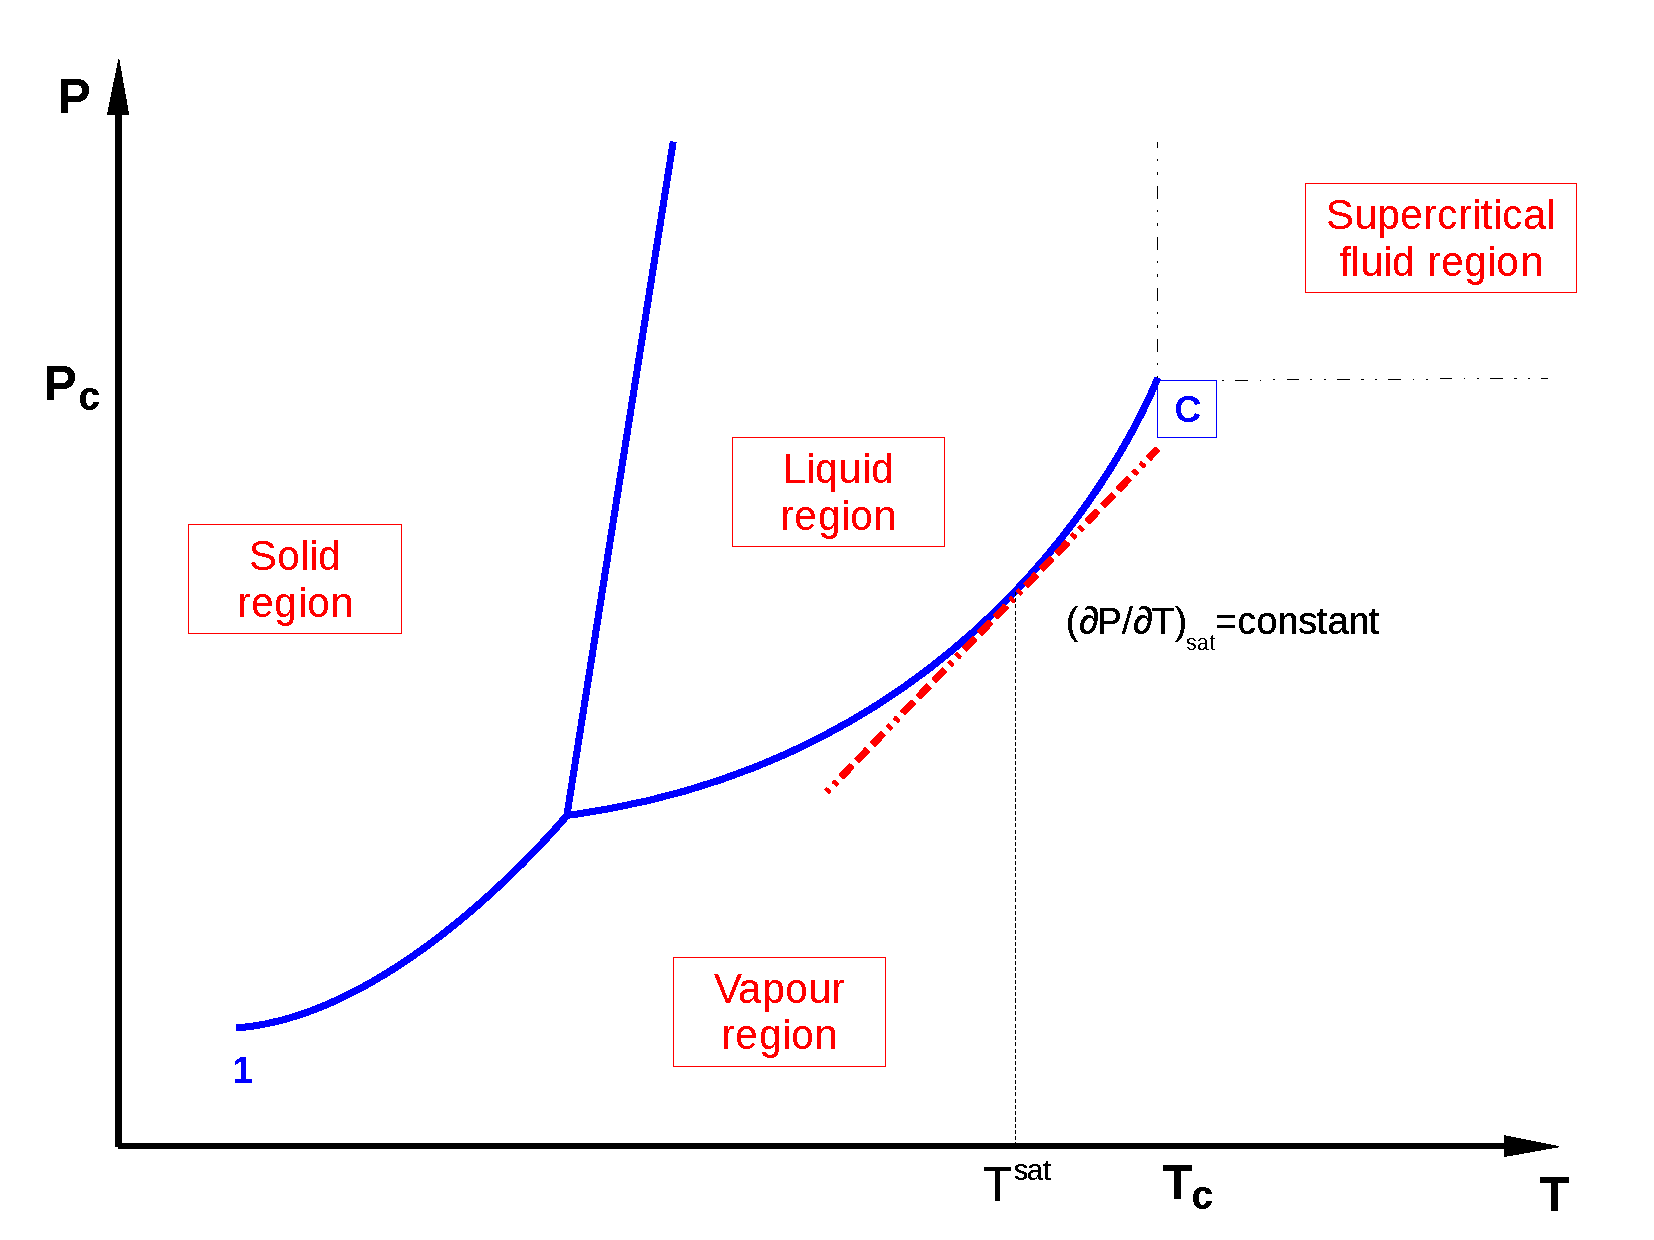
\includegraphics[width=.5\columnwidth,clip]{./../Pics/PT_Diagram2}
               \end{center} 
               \caption{ $PT$ diagrams for a pure substance. Graphical representation of the Clapeyron relation.}\label{Mod03Fig01}
           \end{figure}
      \begin{shaded}
          \begin{equation}
             \frc{d\left(\ln{P^{\text{sat}}}\right)}{dT} = \frc{\Delta H^{\text{fg}}}{RT^{2}} \;\;\Longrightarrow \;\;\; \ln{\left(\frc{P_{2}}{P_{1}}\right)_{\text{sat}}} = \frc{\Delta H^{\text{fg}}}{R}\left(\frc{1}{T_{1}}-\frc{1}{T_{2}}\right)_{\text{sat}}.\label{Mod03_ClausiusClapeyronEqn} 
          \end{equation} 
This expression is known as {\it Clausius-Clapeyron equation} and is a good approximation when describing temperature and pressure dependence at boiling/condensation and at sublimation/gas deposition.
      \end{shaded}
For the dependence of the saturated vapour pressure on $T$, a number of empirical relations have been developed. The simplest expression is,
    \begin{displaymath}
       \ln{P^{\text{sat}}} = A - \frc{B}{T},%\label{Mod03_AntoineSimplest}
    \end{displaymath}
where $A$ and $B$ are constants obtained from experiments. A more `popular' relation is,
    \begin{shaded}
       \begin{equation}
          \ln{P^{\text{sat}}} = A - \frc{B}{T+C},\label{Mod03_Antoine}
       \end{equation}
       this relation is known as {\it Antoine Equation}, where $A$, $B$ and $C$ are constants obtained experimentally.
    \end{shaded}
This two relations, although still widely used by the fluids community are plagued with strong inaccuracy. Due to better accuracy, high-order polynomial relations have become commonly used in flow and process simulators,
    \begin{displaymath}
       \ln{P^{\text{sat}}} = \frc{A\tau + B\tau^{1.5} + C\tau^{3} + D\tau^{6}}{1-\tau}\;\;\;\;\text{ with }\;\;\tau = 1 - T_{r}.
    \end{displaymath}
\end{subequations}


%%% SUBSUBSECTION
   \subsubsection{Vapour-Liquid Equilibrium Systems}

Several processes of engineering relevance occur with fluids in phase equilibria -- either saturated vapour (\ie vapour saturated with liquid droplets) and saturated liquid (\ie liquid saturated with bubbles of vapour). In most cases, it is important to know the actual quantities of both phases in thermodynamic equilibrium, \ie the amount of vapour and liquid present in a constrained system at prescribed temperature and pressure conditions. Let assume that a closed system contains $n$ moles of a chemical species split into $\mathcal{P}$ phases,
    \begin{displaymath}
      n = \sum\limits_{j=1}^{\mathcal{P}} \mfr[n]{}{j} = \mfr[n]{}{1} + \mfr[n]{}{2} + \cdots + \mfr[n]{}{\mathcal{P}}.
    \end{displaymath}
The mass balance acroos all $\mathcal{P}$ phases can be represented as
    \begin{displaymath}
       nV = \mfr[n]{}{1}\mfr[V]{}{1} + \mfr[n]{}{2}\mfr[V]{}{2} + \cdots + \mfr[n]{}{\mathcal{P}}\mfr[V]{}{\mathcal{P}}  = \sum\limits_{j=1}^{\mathcal{P}}\left(nV\right)^{\left(j\right)},
    \end{displaymath}
where $V$ is the molar volume. Dividing by $n$
    \begin{displaymath}
       V = \frc{\mfr[n]{}{1}}{n}\mfr[V]{}{1} + \frc{\mfr[n]{}{2}}{n}\mfr[V]{}{2} + \cdots + \frc{\mfr[n]{}{\mathcal{P}}}{n}\mfr[V]{}{\mathcal{P}}.
    \end{displaymath}
Defining molar (or mole) fraction, $\mfr[x]{}{j}=\frc{\mfr[n]{}{j}}{n}$, where
    \begin{eqnarray}
         && \sum\limits_{j=1}^{\mathcal{P}}\mfr[x]{}{j} = 1,  \nonumber \\
         && V = \mfr[x]{}{1}\mfr[V]{}{1} + \mfr[x]{}{2}\mfr[V]{}{2} + \cdots + \mfr[x]{}{\mathcal{P}}\mfr[V]{}{\mathcal{P}}.  \nonumber
    \end{eqnarray}
For vapour-liquid systems,
    \begin{eqnarray}
         && \mfr[x]{}{L} + \mfr[x]{}{V} = 1,  \nonumber \\
         && V = \mfr[x]{}{L}\mfr[V]{}{L} + \mfr[x]{}{V}\mfr[V]{}{V}. \nonumber
    \end{eqnarray}
For a generic thermodynamic potential $M$ (= $V$, $U$, $H$, $S$ etc),
    \begin{shaded}
       \begin{subequations}
           \begin{equation}
              M = \left(1-\mfr[x]{}{V}\right)\mfr[M]{}{L} + \mfr[x]{}{V}\mfr[M]{}{V}
           \end{equation}
           \begin{equation}
              M = \mfr[M]{}{L} + \mfr[x]{}{V}\Delta\mfr[M]{}{LV}\label{Mod03_QualityVapour}
           \end{equation}
       \end{subequations}
    \end{shaded}
$\mfr[x]{}{V}$ is called \underline{\it vapour quality}. Thermodynamic potentials of pure substances are graphically represented by $Ph$ (pressure $\times$ specific enthalpy) and $Ts$ (temperature $\times$ specific entropy) diagrams, Fig.~\ref{Mod03Fig02}, where information on $P$, $T$, $s$, $h$, $x$ and $v$ (specific volume) can be readily extracted.
%
           \begin{figure}[h]
              \vbox{
                    \hbox{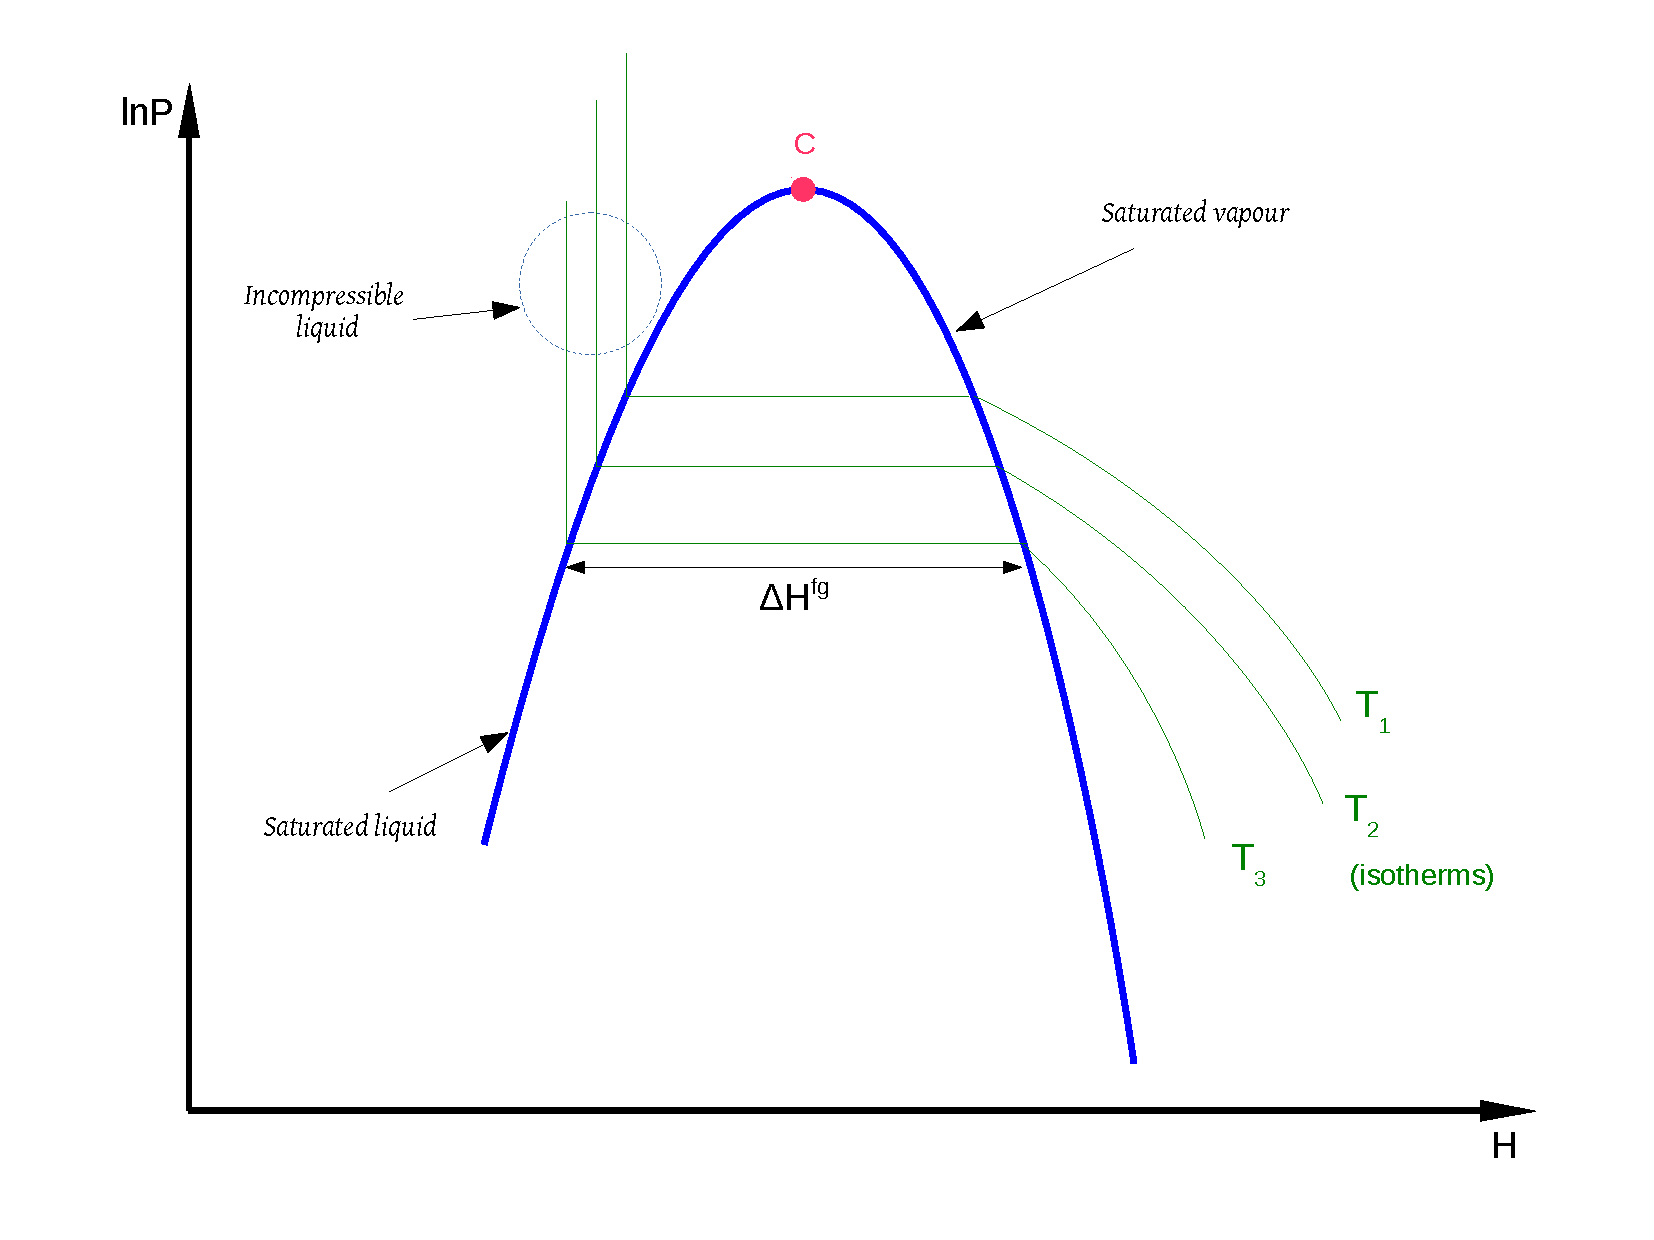
\includegraphics[width=.5\columnwidth,clip]{./Figs/Mod3PHDiagram}
                          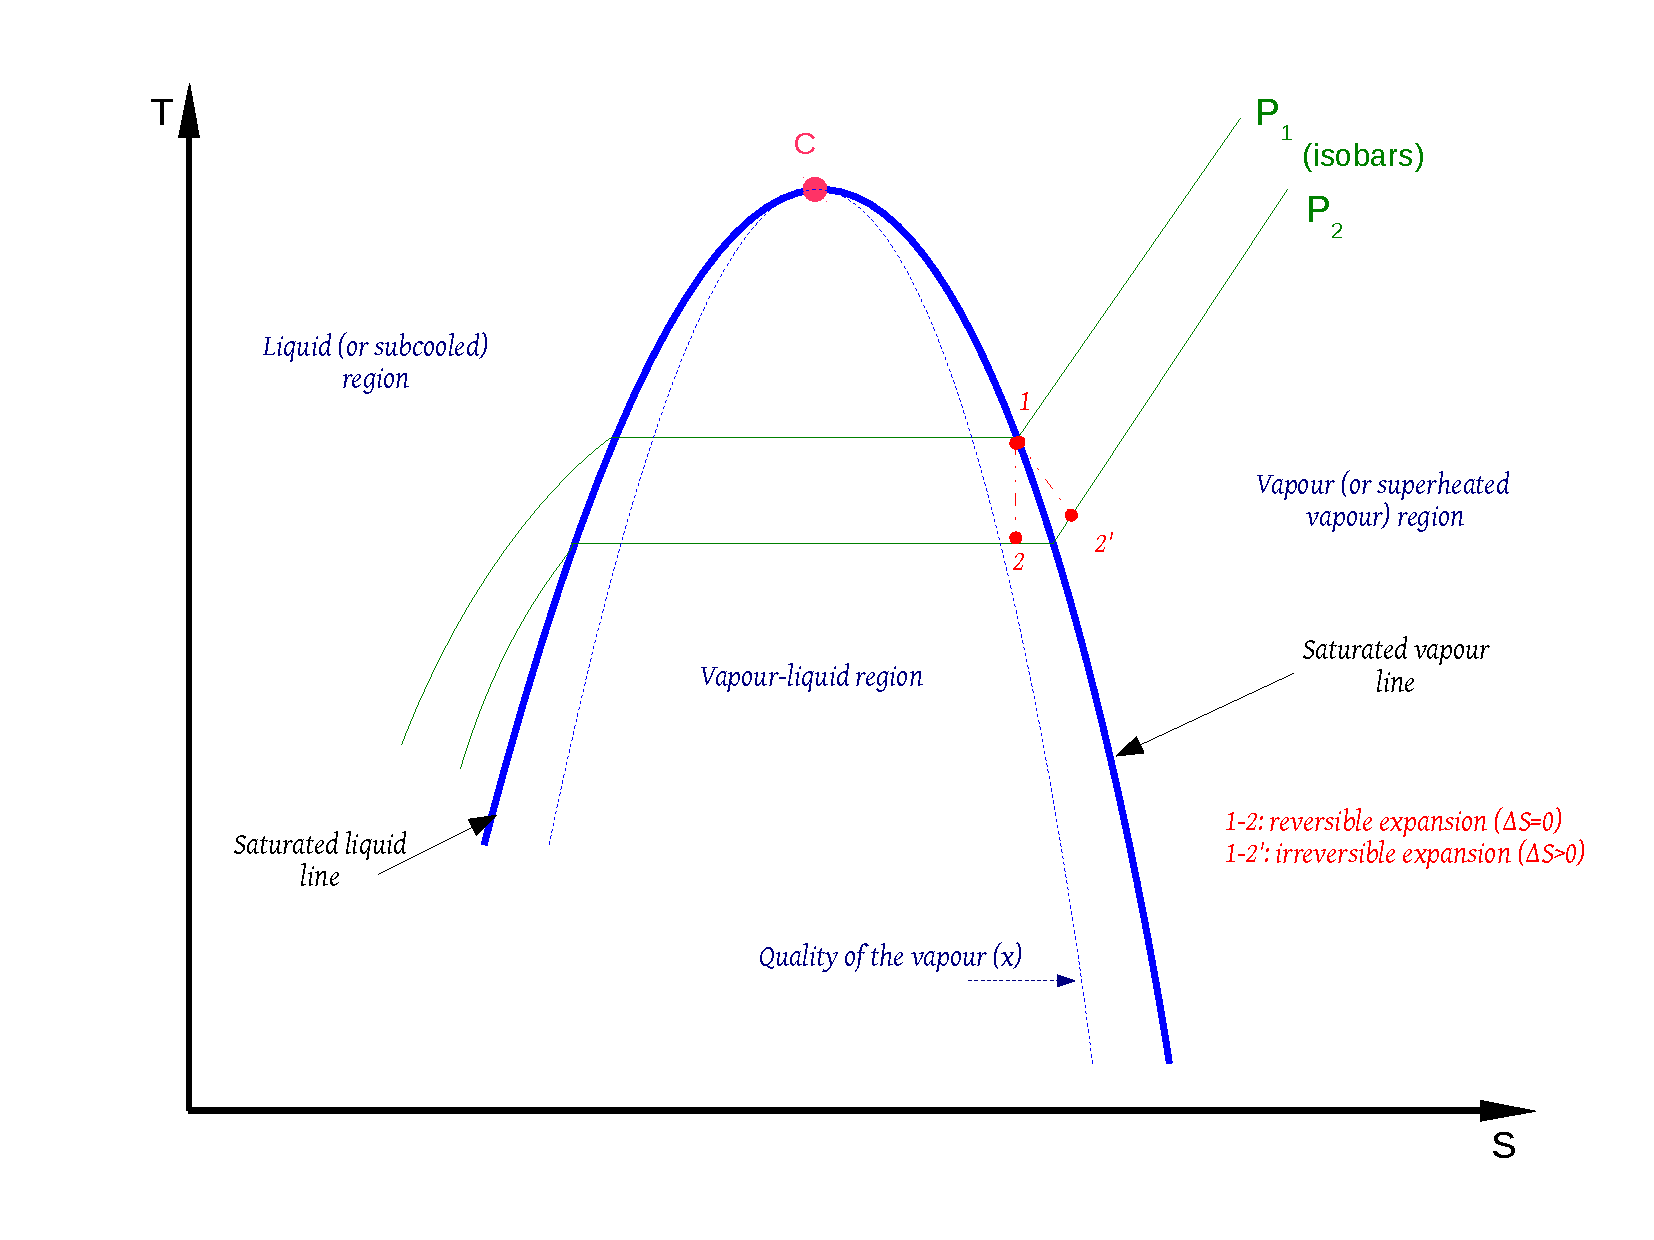
\includegraphics[width=.5\columnwidth,clip]{./Figs/Mod3TSDiagram}}
                    \vspace{-.1cm}
                    \hbox{\hspace{4cm}(a)\hspace{8cm}(b)}}
              \caption{ (a) $Ph$ and (b) $Ts$ diagrams for a pure substance.}\label{Mod03Fig02}
           \end{figure}
%
In the $Ph$ diagram, Fig~\ref{Mod03Fig02}a, isotherms (i.e., lines representing constant temperature) and pressure conditions determine the phase of the fluid. At the left hand-side of the {\it dome} all fluid is at liquid state, whereas at the right hand-side of the {\it dome}, all fluid is at vapour state. The region within the {\it dome} is a two-phase region, where liquid and vapour coexist in thermodynamic equilibrium. As the fluid conditions `move' from the {\it saturated liquid line} to the {\it saturated vapour line} through the {\it isotherm}, the fluid is continuously vaporised `till there is no droplets of liquid fluid. The total amount of heat given to the system -- $\Delta H^{\text{fg}}$, is the latent heat of vaporisation. In a similar way, the $Ts$ diagram, Fig~\ref{Mod03Fig02}b, shows similar features over different {\it isobars}. In addition, the {\it quality} of the vapour can also be graphically represented. In a reversible expansion from $P_{1}$ to $P_{2}$ $\left(P_{1}>P_{2}\right)$, entropy change is null, $\Delta s=0$, and is represented by a vertical line, however during irreversible expansion, $\Delta s >0$, represented by an inclined line.  

 $Ph$ and $Ts$ diagrams for common substances are no longer used by industry but it helps to qualitatively understand phase (and associated thermodynamic potentials) behaviour of pure substances. Quantitative information can be obtained from either saturated and superheated (Fig.~\ref{Mod03Fig03}) fluid tables or dedicated software, \eg
\begin{itemize}
   \item \href{http://www.weatherford.com/doc/wft183650}{PVTflex$^{TM}$};
   \item \href{http://www.kbcat.com/infochem-software/flow-assurance-software-multiflash/pvt-simulation}{Multiflash$^{TM}$};
   \item \href{https://www.honeywellprocess.com/en-US/explore/products/advanced-applications/unisim/Pages/default.aspx}{UniSim – Software for Process Design and Simulation};
   \item \href{http://webbook.nist.gov/chemistry/fluid/}{NIST Website}
   \item etc.
\end{itemize}
In general, table of {\it saturated fluid properties}, Fig.~\ref{Mod03Fig03}a, contains information of the fluid within the {\it dome}, whereas the table of {\it superheated fluid properties} refer to the region outside (rhs) the {\it dome}. 
%
   \begin{figure}[h]
      \vbox{
         \hbox{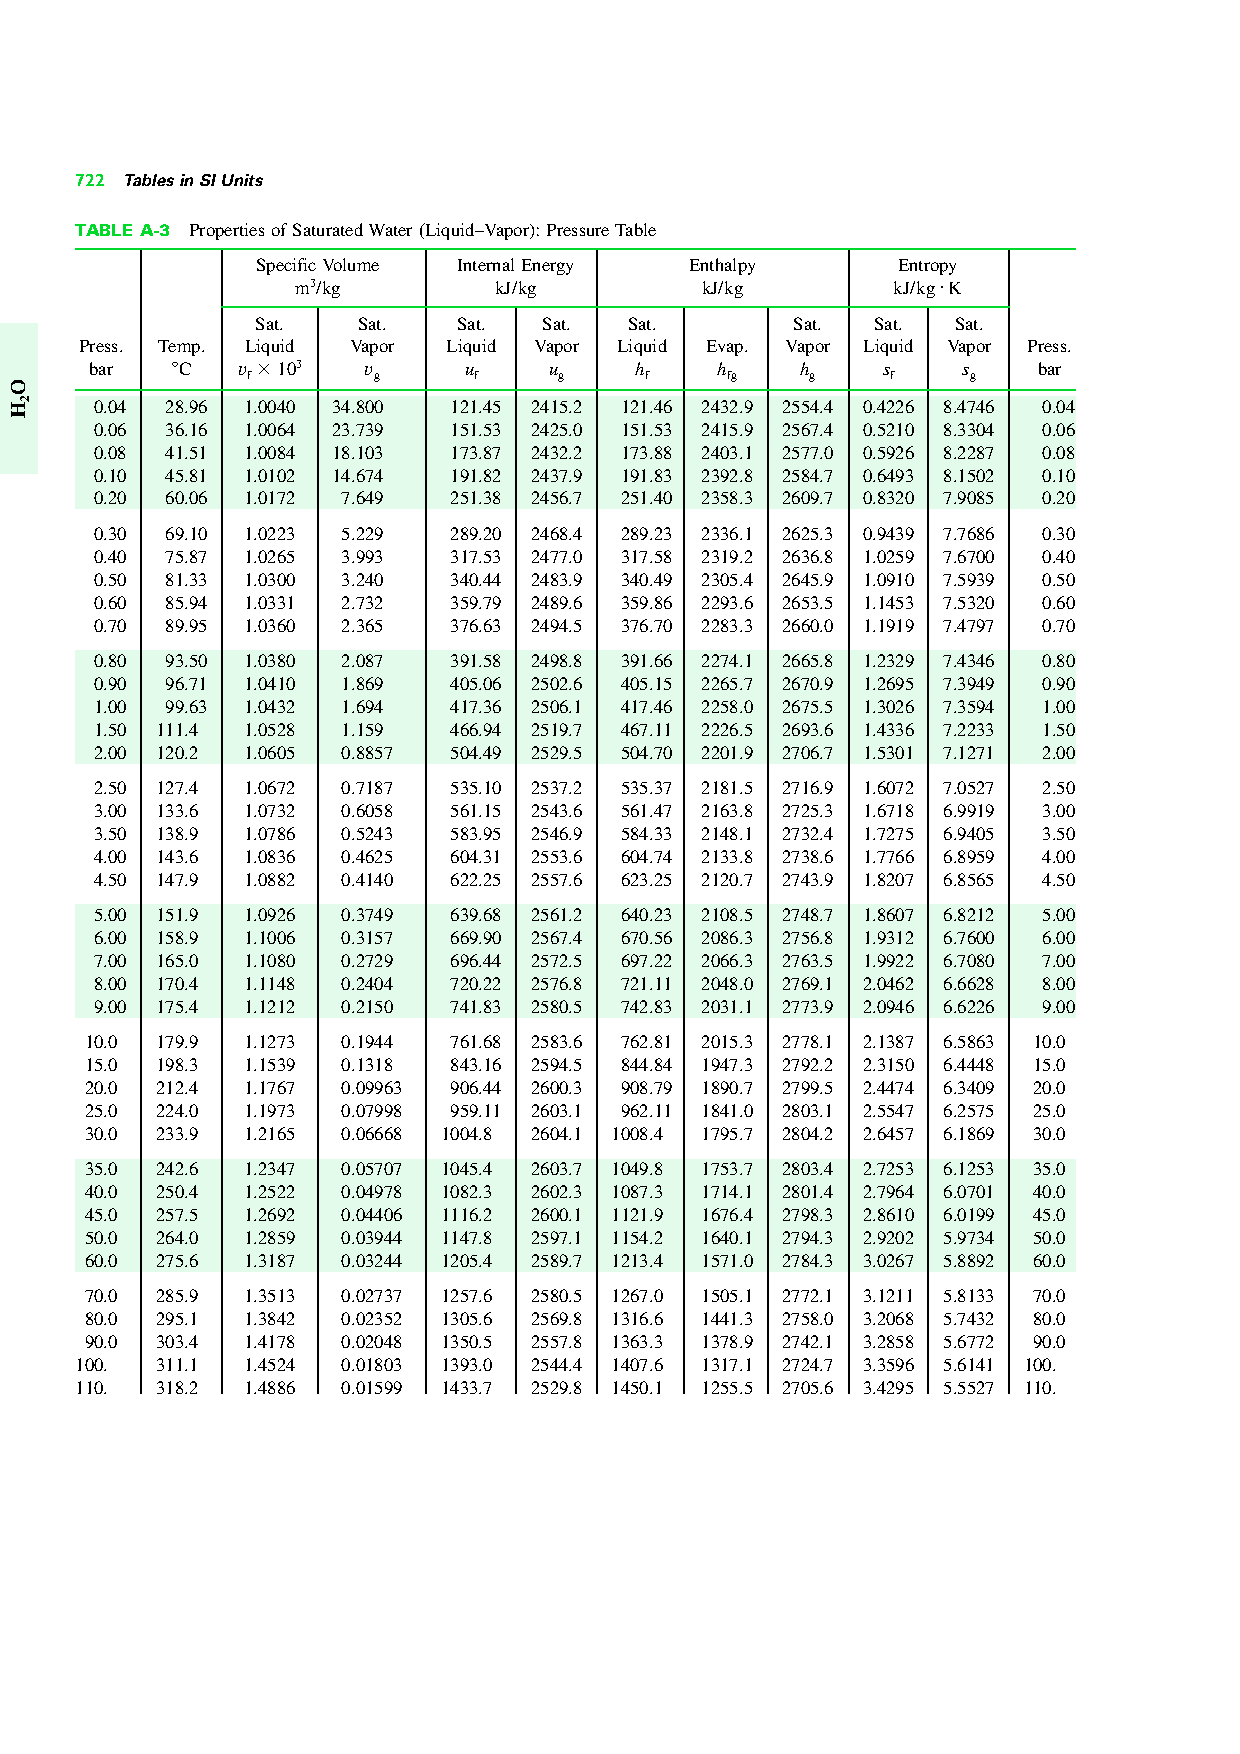
\includegraphics[width=.5\columnwidth,clip]{./Figs/WaterSatTable}
               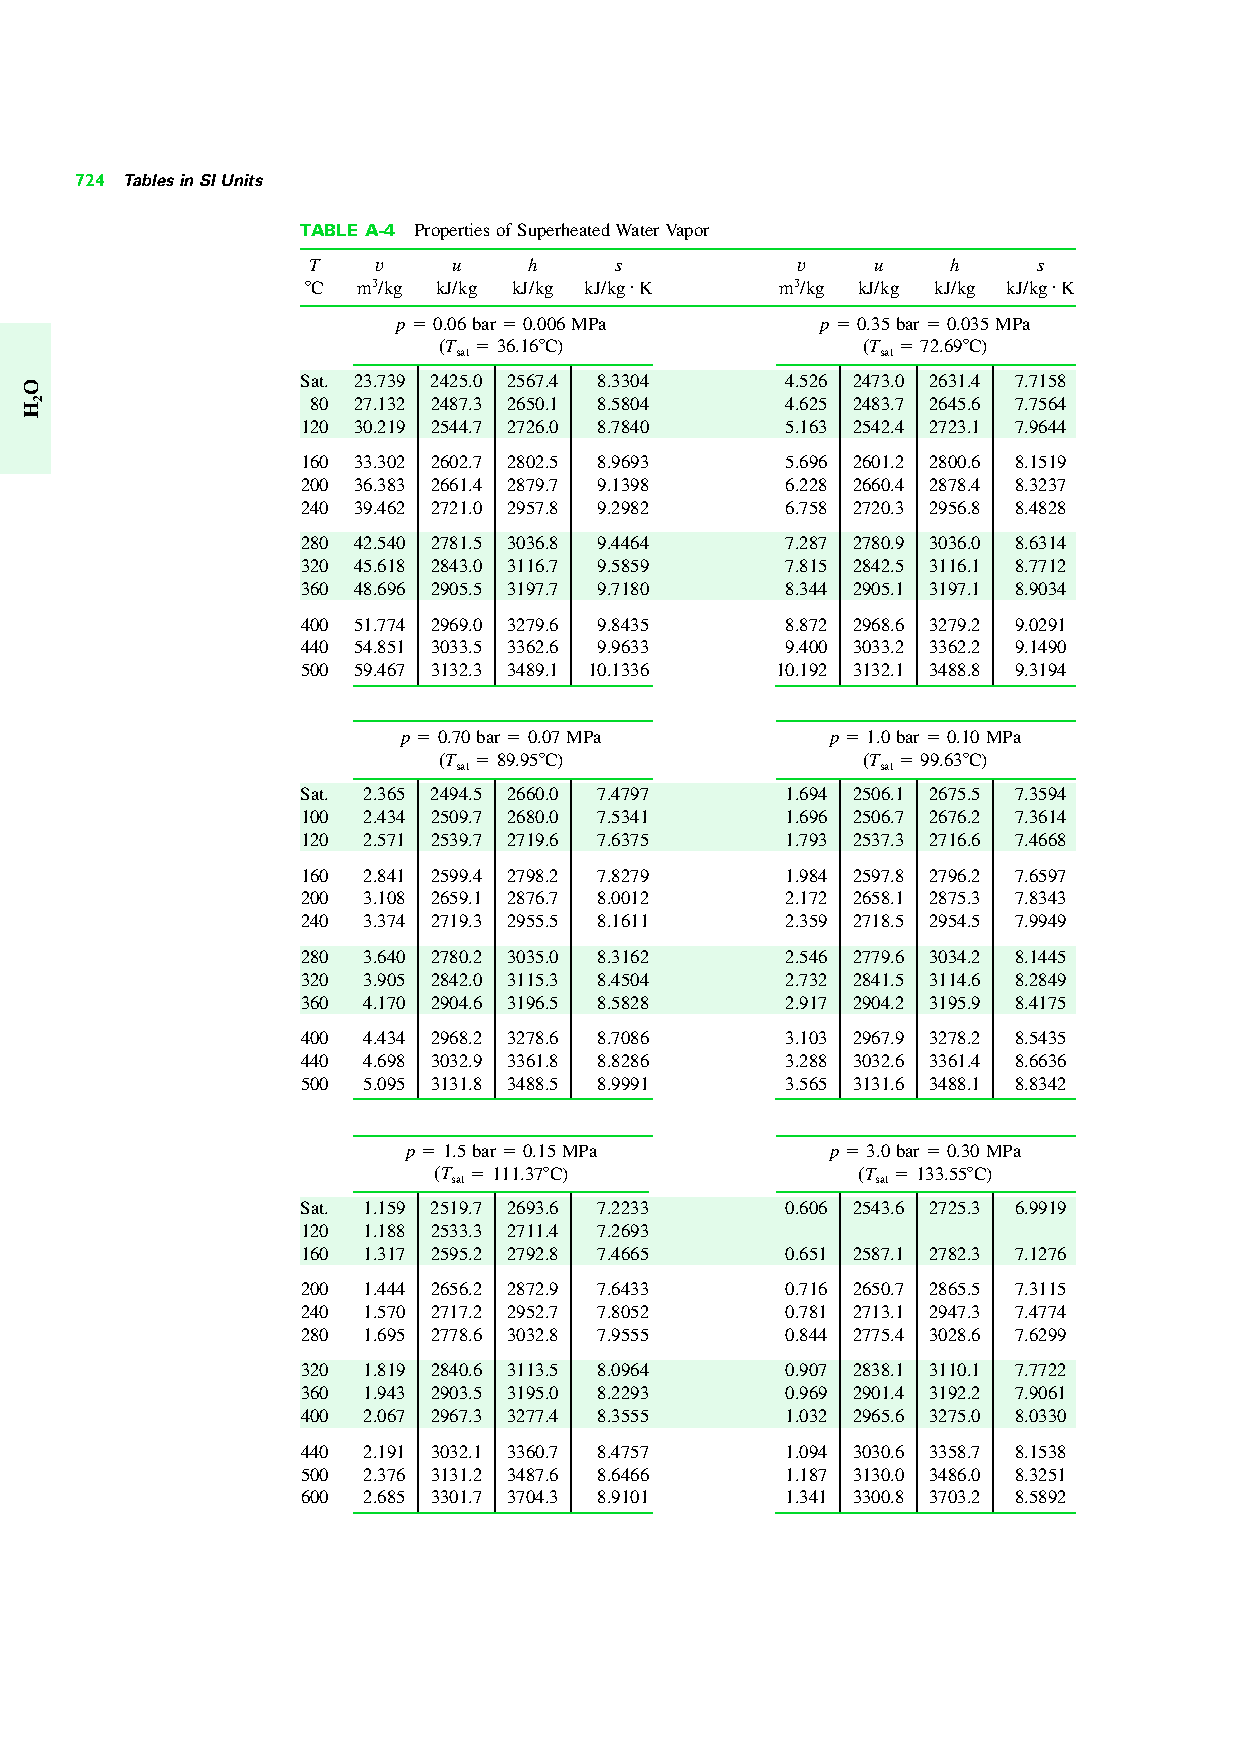
\includegraphics[width=.5\columnwidth,clip]{./Figs/Water_SuperheatedTable}}
         \vspace{-1.5cm}
         \hbox{\hspace{4cm}(a)\hspace{7cm}(b)}
      }
      \caption{ Table of properties of (a) saturated water-steam and (b) superheated vapour (Extracted from Moran $\&$ Saphiro, see Appendix B).}\label{Mod03Fig03}  
   \end{figure}
%
    

%%% SUBSUBSECTION
   \subsubsection{Industrial Applications: Power System}
Regardless the energy source (fossil fuel, nuclear or geothermal), power plants are good applications for VLE systems as fluids are continuously vaporised and condensed by addition and extraction of heat and volume expansion. {\it Rankine thermal cycles} are system configurations for generating power and consist of four processes (Fig.~\ref{Mod03Fig04}) with associated energy balances:
     \begin{itemize}
      \item \textcolor{red}{Process 1-2}: reversible adiabatic (i.e., \blue{isentropic}) expansion in the turbine (or steam engine),
            \begin{displaymath}
               \left(h_{2} + \dot{W}_{T}\right)-h_{1} = 0 \Rightarrow \dot{W}_{T} = h_{1}-h_{2}
            \end{displaymath}
      \item \textcolor{red}{Process 2-3}: constant-pressure heat transfer (to the environment) in the condenser,
            \begin{displaymath}
               \left(h_{3} + \dot{Q}_{C}\right)-h_{2} = 0 \Rightarrow \dot{Q}_{C} = h_{2}-h_{3}
            \end{displaymath}
      \item \textcolor{red}{Process 3-4}: reversible adiabatic (i.e., \blue{isentropic}) pumping process in the feed pump,
            \begin{displaymath}
               h_{4} - \left(h_{3} + \dot{W}_{P}\right) = 0 \Rightarrow \dot{W}_{P} = h_{4}-h_{3}
            \end{displaymath}
      \item \textcolor{red}{Process 4-1}: constant-pressure heat transfer (to the fluid) in the boiler,
            \begin{displaymath}
               h_{1} - \left(h_{4} + \dot{Q}_{B}\right) = 0 \Rightarrow \dot{Q}_{B} = h_{1}-h_{4}
            \end{displaymath} 
     \end{itemize}
     The efficiency $\left(\eta\right)$ of the Rankine cycle is given by
           \begin{displaymath}
               \eta_{\text{Rankine}} = \frc{\sum W_{i}}{Q_{B}} = \frc{\left|W_{\text{net}}\right|}{Q_{B}} = \frc{\left|\left(h_{1}-h_{2}\right)+\left(h_{4}-h_{3}\right)\right|}{h_{1}-h_{4}}.
           \end{displaymath}
     Due to engineering constraints, fluids entering and leaving the pump \underline{must be} at liquid phase, thus $h_{4}=h_{f4}$ and $h_{3}=h_{f3}$, \ie the fluid has the enthalpy of the liquid phase (from the saturated fluid table) at the prescribed temperature and pressure conditions. {\it Pumps} are able to induce the transport of liquid fluids that are often assumed incompressible, therefore
          \begin{displaymath}
                Tds = dh - v dP
          \end{displaymath}
as the compression occurs isentropically, \ie $ds=0$,
          \begin{displaymath}
                dh = v dP \Rightarrow h_{f4} = h_{f3} + v_{3}\left(P_{4}-P_{3}\right).
          \end{displaymath}
However, as $\left(h_{f4}-h_{f3}\right) <<<<< \left(h_{1}-h_{2}\right)$, the efficiency can be considered as
           \begin{displaymath}
               \eta_{\text{Rankine}} = \frc{\left|\left(h_{1}-h_{2}\right)\right|}{h_{1}-h_{f4}}.
           \end{displaymath}     
%
   \begin{figure}[h]
      \begin{center}
         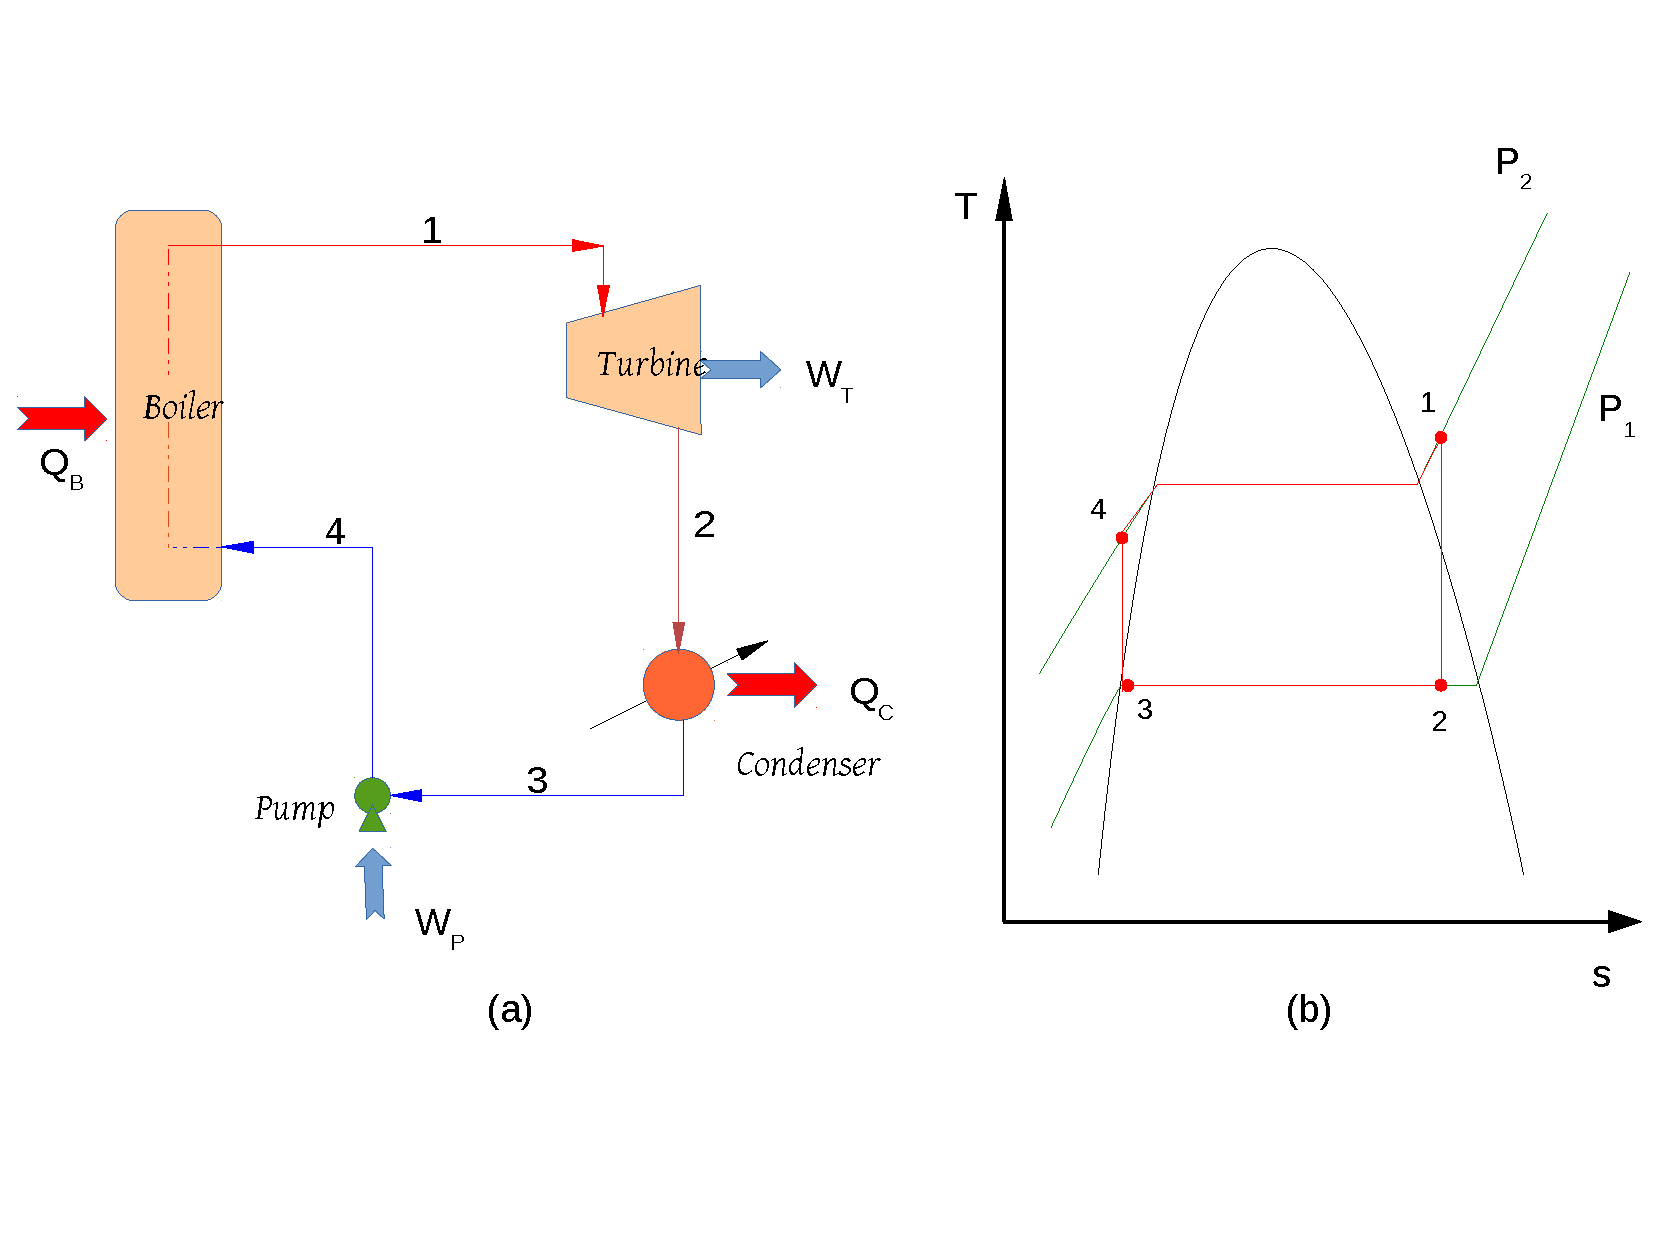
\includegraphics[width=\columnwidth,clip]{./Figs/Mod3PowerSystemDiagram}
      \end{center}
      \caption{ (a) Diagram of Rankine thermal cycle for power generation and associated $Ts$ diagram.}\label{Mod03Fig04}
   \end{figure}


\clearpage

%%% SUBSECTION
\subsection{Examples}

\begin{enumerate}[1)]
%%%
%%% EXAMPLE 
%%%
\item\label{Mod03Ex01} A block of copper of 1 kg undertakes a reversible compression from 0.1 MPa to 100 MPa at constant temperature of 15$^{\circ}$C. Calculate:
    \begin{enumerate}[a)]
       \item Work done on the copper block during the process;
       \item Change in entropy {\it per} kg of copper;
       \item Heat transfer and;
       \item Change of internal energy {\it per} kg.
    \end{enumerate}
    Given, 
    \begin{itemize}
       \item Volume expansivity coefficient: $\beta = 5\times 10^{-5}$ K$^{-1}$;
       \item Isothermal compressibility coefficient: $\kappa = 8.6\times 10^{-12}$ m$^{2}$.N$^{-1}$;
       \item specific volume: $v=1.14\times 10^{-4}$ m$^{3}$.kg$^{-1}$.
    \end{itemize} 

% SOLUTION
    \noindent{\bf Solution:} 
       \begin{enumerate}[a)]
%
            \item The work done during the compression,
                \begin{displaymath}
                   w = -\int P dv,
                \end{displaymath}
                where $v$ is the specific volume. $\kappa$ was defined in Module~\ref{Section:02} as,
                \begin{displaymath}
                   \kappa = \frc{1}{v}\left(\frc{\partial v}{\partial P}\right)_{T}\;\Longrightarrow \; v\kappa dP = - dv \;\;\text{ (with constant T)}
                \end{displaymath}
                For isothermal processes
                \begin{displaymath}
                   w = -\int P dv = - \int P\left(-v\kappa dP\right) = \frc{v}{2}\kappa\left(P_{2}^{2}-P_{1}^{2}\right) = 4.90 \frc{\text{J}}{\text{kg}}
                \end{displaymath}
%
            \item $ds$ = ? (specific entropy).\\
                  From the Maxwell relations -- Eqn.~\ref{Mod03_MaxwellRelation4}, 
                \begin{displaymath}
                   -\left(\frc{\partial s}{\partial P}\right)_{T} = \left(\frc{\partial v}{\partial T}\right)_{P},
                \end{displaymath}
                and from the definition of $\beta$,
                \begin{eqnarray}
                    && \beta = \frc{1}{v}\left(\frc{\partial v}{\partial T}\right)_{P} \;\;\Longrightarrow\;\; -\left(\frc{\partial s}{\partial P}\right)_{T} = \beta v \nonumber \\
                    && ds = -\beta v dP \;\;\Longrightarrow ds = s_{2}-s_{1} = -\beta v \left(P_{2}-P_{1}\right) = -0.5694 \frc{\text{J}}{\text{kg.K}} \nonumber
                \end{eqnarray}
%
            \item The heat transferred in such reversible isothermal process is
                \begin{displaymath}
                   dq = Tds \;\;\Longrightarrow q = T\left(s_{2}-s_{1}\right) = -164.07 \frc{\text{J}}{\text{kg}}.
                \end{displaymath}
%
            \item The specific internal energy,
                \begin{eqnarray}
                   &&  du = q + w \nonumber \\
                   && \left(u_{2}-u_{1}\right) = \underbrace{-164.07}_{\text{heat removed from the system}} + \overbrace{4.90}^{\text{work given to the system}} = -159.17 \frc{\text{J}}{\text{kg}}. \nonumber
                \end{eqnarray}
 
%
       \end{enumerate} 

\clearpage
%%%
%%% EXAMPLE 
%%%
\item\label{Mod03Ex02} Demonstrate that the derivative of molar volume \wrt temperature at constant pressure is
     \begin{displaymath}
         \Partial[V]{T}{P} = -\frc{\Partial[P]{T}{V}}{\Partial[P]{V}{T}},
     \end{displaymath}
     and obtain an expression for $\Partial[V]{T}{P}$ for the van der Waals EOS. {\bf Hint:} You should start the proof from the total differential of a continuous function $f(a,b)$,
     \begin{displaymath}
         df = \Partial[f]{a}{b}da + \Partial[f]{b}{a}db.
     \end{displaymath}

% SOLUTION
    \noindent{\bf Solution:} The total differential of a generic continuous function $f(a,b)$ is
     \begin{displaymath}
         df = \Partial[f]{a}{b}da + \Partial[f]{b}{a}db.
     \end{displaymath}
     where (from the given thermodynamic function) $f=P$, $a=T$ and $b=V$, \ie
     \begin{displaymath}
         dP = \Partial[P]{T}{V}dT + \Partial[P]{V}{T}dV.
     \end{displaymath}
     However we want a differential expression in which $P$ is constant, therefore $dP = 0$,
     \begin{eqnarray}
         0 &=& \Partial[P]{T}{V}dT + \Partial[P]{V}{T}dV \;\;\;\text{ at } P \text{ constant},\nonumber \\
         \Partial[V]{T}{P} &=& -\frc{\Partial[P]{T}{V}}{\Partial[P]{V}{T}}.\nonumber
     \end{eqnarray}

     \medskip\noindent
     The vdW-EOS is,
     \begin{displaymath}
          P = \frc{RT}{V-b} - \frc{a}{V^{2}},
     \end{displaymath}
     where $V$ is the molar volume and $a$ and $b$ are constants that {\it depends only on critical properties}, $P_{c}$ and $T_{c}$. Due to the non-linearity of this EOS, obtaining $\Partial[V]{T}{P}$ from a direct differentiation would be difficult. However, we can use the expression that we just derived,
     \begin{displaymath}
         \Partial[V]{T}{P} = -\frc{\Partial[P]{T}{V}}{\Partial[P]{V}{T}} = -\frc{\frc{R}{V-b}}{-\frc{RT}{\left(V-b\right)^{2}}+\frc{2a}{V^{3}}}
     \end{displaymath} 

\clearpage
%%%
%%% EXAMPLE 
%%%
\item\label{Mod03Ex03} The Antoine equation constants for toluene are $A=14.01415$, $B=3106.46$ K and $C=-53.15$ K (for pressure given in kPa). At 1.01325$\times$10$^{5}$ Pa, calculate the boiling temperature and the enthalpy of vaporisation at this temperature.

% SOLUTION
    \noindent{\bf Solution:} Boiling temperature can be calculated from the Antoine equation,
       \begin{displaymath}
          \ln{P^{\text{sat}}} = A - \frc{B}{T+C} \;\;\;\Rightarrow \;\;\; T = \frc{B}{A-\ln{P^{\text{sat}}}} - C = \red{383.77 K}
       \end{displaymath}
The enthalpy of vaporisation, $\Delta H^{\text{fg}}$, can be obtained from the Clausius-Clapeyron equation,
         \begin{eqnarray}
            \frc{d}{dT} \left(\ln{P^{\text{sat}}}\right) &=& \frc{\Delta H^{\text{fg}}}{RT^{2}} \nonumber \\
             \frc{B}{\left(T+C\right)^{2}} &=&  \frc{\Delta H^{\text{fg}}}{RT^{2}} \;\;\Longrightarrow \Delta H^{\text{fg}} = 34.7984 \text{kJ.mol}^{-1}. \nonumber
         \end{eqnarray}
 
\clearpage

%%%
%%% EXAMPLE 
%%%  
\item\label{Mod03Ex04} Derive an expression for enthalpy change of a gas during an isothermal process assuming using the following EOS: $P\left(V-b\right)=RT$

% SOLUTION
    \noindent{\bf Solution:} We have seen that enthalpy change is given by Eqn.~\ref{Mod03_DerivedEnthalpyRelation1},
    \begin{displaymath}
       dH = C_{p}dT + \left[V - T\Partial[V]{T}{P}\right]dP.
    \end{displaymath}
    We can rearrange the given EOS and obtain $\Partial[V]{T}{P}$,
    \begin{eqnarray}
       && P\left(V-b\right)=RT \;\;\;\rightarrow\;\;\; V = \frc{RT}{P} + b \;\;\;\rightarrow\;\;\; \Partial[V]{T}{P} = \frc{R}{P}\;\;\text{ thus, } \nonumber \\
       && dH = C_{p}dT + \left(V - \frc{RT}{P}\right)dP = \blue{C_{p}dT + bdP}. \nonumber 
    \end{eqnarray}
    
\clearpage
    
\clearpage
 
%%%
%%% EXAMPLE 
%%%  
\item\label{Mod03Ex06} Steam (dry and saturated) is supplied by the boiler at 15 bar and the condenser inlet pressure is 0.4 bar. Calculate the Rankine efficiency of the cycle. Neglect the pump work, assume the enthalpy of fluid leaving the pump is 317.58 kJ.kg$^{-1}$

% SOLUTION  
    \noindent{\bf Solution:} At 15 bar, dry and saturated $\left(\ie x_{1}=1\right)$ steam has the following properties (from saturated table)\footnote{Using the same numbering as in Fig.~\ref{Mod03Fig04}.},
          \begin{eqnarray}
             T_{1} &=& T_{\text{sat}} = 198.3^{\circ}\text{C},\nonumber \\
             h_{1} &=& h_{\text{g}} = 2792.2\; \text{kJ.kg}^{-1} \nonumber \\
             s_{1} &=& s_{\text{g}} = 6.4448\; \text{kJ.(kg.K)}^{-1} \nonumber
          \end{eqnarray} 
    In the condenser, $P_{2}=0.4$ bar,
          \begin{eqnarray}
              T_{2} &=& T_{\text{sat}} = 75.87^{\circ}\text{C}, \nonumber \\
              h_{\text{g}2} &=& 2636.8\;\text{kJ.kg}^{-1},\;\;\; h_{\text{f}2} = 317.58\;\text{kJ.kg}^{-1},  \nonumber \\
              s_{\text{g}2} &=& 7.6700 \;\text{kJ.(kg.K)}^{-1},\;\;\; s_{\text{f}2} = 1.0259\;\text{kJ.(kg.K)}^{-1}. \nonumber  
          \end{eqnarray}
$h_{2}$ and $s_{2}$ depend on the knowledge of how vaporised the water is, in other words, we need to determine the quality of the steam, $x_{1}$ through Eqn.~\ref{Mod03_QualityVapour},
      \begin{eqnarray}
          h_{2} &=& h_{\text{f}2} + x_{2}\left(h_{\text{g}2} - h_{\text{f}2}\right), \nonumber \\
          s_{2} &=& s_{\text{f}2} + x_{2}\left(s_{\text{g}2} - s_{\text{f}2}\right). \nonumber
      \end{eqnarray}
As we know that water is expanded isentropically in the turbine, \ie $s_{1}=s_{2}$,
      \begin{displaymath}
         s_{2} = s_{\text{f}2} + x_{2}\left(s_{\text{g}2} - s_{\text{f}2}\right) = s_{1} = 6.4448 \;\;\;\Rightarrow \;\;\; x_{2} = 0.8156 \;\;(81.56\% \text{ of vapour}
      \end{displaymath}
Thus replacing in 
      \begin{displaymath}
          h_{2} = h_{\text{f}2} + x_{2}\left(h_{\text{g}2} - h_{\text{f}2}\right) = 2209.14\text{ kJ.kg}^{-1}.
      \end{displaymath}
The Rankine efficiency is given by
      \begin{displaymath}
           \eta_{\text{Rankine}} = \frc{\text{Adiabatic or Isentropic Heat Drop}}{\text{Heat Supplied}} = \frc{\left|h_{1}-h_{2}\right|}{h_{1}-h_{\text{f}4}} = 0.2356\;\;\;\rightarrow \;\;\; 23.56\%
      \end{displaymath}
    


\end{enumerate}


\clearpage
%%%%%%%%%%%%%%%%%%%%%%%%%%%%%%%%%%%%%%%%%%%%%%%%%%%%%%%%%%%%%%%%%%%%%%%%%%%%%%%%%%%%%%%%%%%%%%%%%%%%%%%%%%%%%%%%%%%%%%%%%%%%%%%%%%%%%%%%%%%%%%
%%%%%%%%%%%%%                                                    END OF MODULE 03                                                %%%%%%%%%%%%%
%%%%%%%%%%%%%%%%%%%%%%%%%%%%%%%%%%%%%%%%%%%%%%%%%%%%%%%%%%%%%%%%%%%%%%%%%%%%%%%%%%%%%%%%%%%%%%%%%%%%%%%%%%%%%%%%%%%%%%%%%%%%%%%%%%%%%%%%%%%%%%

%%%
%%% SECTION
%%%
\section{Module 04: Vapour-Liquid Equilibrium of Mixtures}\label{Section:04}

Up to this point, we have only considered thermodynamic and volumetric properties of pure components at prescribed pressure and temperature conditions. However, most engineering applications deals with mixtures of components that may be present in single or multiple phases, \eg oil in reservoirs, naphtha distillation, steel processing etc. This module focuses on understanding PVT behaviour of mixtures and the conditions for vapour-liquid equilibrium (VLE).


%%% SUBSECTION
\subsection{A Few Important Definitions}


%%% SUBSUBSECTION
\subsubsection{Representing Compositions}\label{Section:04:Compositions}
In the previous modules, we mostly focused on thermodynamic properties of systems containing pure chemical species. This module (and the remaining of the course) will study systems with arbitrary number of components, and the quantification of each component at each phase. For a mixture containing $\mathcal{C}$ chemical species, each of them with an arbitrary number of moles, $n_{i},\;\;\forall i\in\left\{1,2,\cdots,\mathcal{C}\right\}$, 
\begin{subequations}
   \begin{enumerate}[a)]
       \item Molar (or mole) $\left(x_{i}\right)$ fraction:
            \begin{eqnarray}
                x_{i} = \frc{n_{i}}{n}.
            \end{eqnarray} 
            where $n=\summation[n_{i}]{i=1}{\mathcal{C}}$ is the total number of moles in the system. As the molar fraction is normalised, we can define:
            \begin{equation}
                  \summation[x_{i}]{i=1}{\mathcal{C}} = 1,
            \end{equation}
       \item (Average) Molar mass of mixtures:
            \begin{equation}
                \overline{MW} = \summation[\left(x_{i} \cdot MW_{i}\right)]{i=1}{\mathcal{C}}
            \end{equation}
         where $MW_{i}$ is the molecular weight (or molar mass) of species $i$.
   \end{enumerate}
\end{subequations}

%%% SUBSUBSECTION
\subsubsection{Partial Molar Properties}\label{Section:04:PartialMolarProperties}

{\it Partial molar properties} describes the behaviour of homogeneous multi-component systems. Let's consider a homogeneous (\ie single phase) and open system (\ie system that allows mass and energy transfer across the boundary towards the surroundings) that undertakes a change in composition. Thus, the total value of any extensive property $M^{\text{t}}\;\left(M\equiv V, U, H, S, G, A\right)$ is not only a function of pressure and temperature, but it also depends on the number of moles of each species in the system. therefore
  \begin{subequations}
     \begin{equation}
        M^{\text{t}} = nM = M\left(T,P,n_{1},n_{2},\cdots, n_{\mathcal{C}}\right).\label{Mod04_PartialProperties1}
     \end{equation}
     The total derivative of Eqn.~\ref{Mod04_PartialProperties1} is,
     \begin{displaymath}  
        d(nM) = \Partial[(nM)]{P}{T,n}dP + \Partial[(nM)]{T}{P,n}dT + \Partial[(nM)]{n_{i}}{T,P,n_{j\ne i}}dn_{i},
     \end{displaymath}
     where the subscript $n$ in the partial derivatives indicates that the number of moles is kept constant, whereas $n_{j\ne i}$ indicates that the number of moles of all components, except component $i$, are kept constant. This expression can be simplified to be a function of the mole fraction, $x_{i}$,
     \begin{shaded}
        \begin{equation}  
           d(nM) = n\Partial[M]{P}{T,x}dP + n\Partial[M]{T}{P,x}dT + \summation[\overline{M}_{i}dn_{i}]{i}{},\label{Mod04_PartialProperties2}
        \end{equation}
     \end{shaded}
     \noindent where $\overline{M}_{i} = \Partial[(nM)]{n_{i}}{T,P,n_{j\ne i}}$ defines the {\it partial molar property} $\overline{M}_{i}$ of species $i$ in solution, \ie the change of the total property $nM$ of a mixture of $\mathcal{C}$ species resulting from the addition at constant $T$ and $P$ of infinitesimal amount of species $i$ to a prescribed amount of solution. We will discuss partial molar properties in more details in Module~\ref{Section:05}.
  \end{subequations}

%%% SUBSUBSECTION
\subsubsection{Excess Properties}\label{Section:04:ExcessProperties}
  
In Section~\ref{Section:03:ResidualProperties}, we have defined {\it residual properties} for gases as the difference between any extensive thermodynamic property, $M$, in real gases and its equivalent assuming ideal gas behaviour, $M^{\text{ig}}$. The equivalent for liquids is called {\it excess properties}, \ie the deviation from an ideal liquid solution property.

Let's assume that $M$ is any extensive thermodynamic property (\eg $V$, $U$, $H$, $S$, $G$ and $A$), the excess property $M^{\text{E}}$ is defined as the difference between the property value of a solution and the value it would have as an ideal solution at the same $T$, $P$ and composition,
\begin{subequations}
  \begin{shaded}
    \begin{equation}
       M^{\text{E}} \equiv M - M^{\text{id}},\label{Mod04_ExcessProperties1a}
    \end{equation}
  \end{shaded}
  \noindent where properties in ideal ({\it id}) solutions of multiple chemical species can be represented as,
    \begin{displaymath}
       M^{\text{id}} = \summation[x_{i}M_{i}]{i}{},
    \end{displaymath}
    where $M_{i}$ is an extensive {\it molar property of the \underline{pure} chemical species}. For example, if we mix equal volumes of two species (\eg water and ethanol), the final volume \underline{is not} the sum of the individual volumes. In fact, the final volume will be slightly larger than the sum of the individual volumes and this is due to the non-ideality behaviour of real liquid fluids. Thus for a binary solution,
    \begin{equation}
      V^{\text{E}} = V - V^{\text{id}} = V - \summation[x_{i}V_{i}]{i}{} = V -\left(x_{1}V_{1}+x_{2}V_{2}\right).\label{Mod04_ExcessProperties1b} 
    \end{equation}
    %This equation shows that the total volume of a mixture of two components is different from the simple addition of both individual volumes. 
\end{subequations}



%%% SUBSECTION
\subsection{Criteria for Chemical Equilibrium}\label{Section:04:ChemicalEquilibrium}

  
%%% SUBSUBSECTION
\subsubsection{Chemical Potential $\left(\mu_{i}\right)$}\label{Section:04:ChemicalPotential}

If we apply the concept of partial molar property to the Gibbs free energy definition, assuming that this thermodynamic potential is a function of $P$, $T$ and $n$, \ie $G^{\text{t}}= nG = G\left(T,P,n_{1},n_{2},\cdots,n_{\mathcal{C}}\right)$,
  \begin{subequations}
      \begin{equation}
         d(nG) = n\Partial[G]{P}{T,x}dP + n\Partial[G]{T}{P,x}dT + \summation[\overline{G}_{i}dn_{i}]{i}{}.\label{Mod04_ChemPotentialDef1}
      \end{equation}
      By definition the {\it partial molar Gibbs free energy} is called \blue{chemical potential $\left(\mu_{i}\right)$},
      \begin{shaded}
         \begin{equation}
            \mu_{i} = \Partial[(nG)]{n_{i}}{T,P,n_{j\ne i}} \;\;\Longleftrightarrow\;\; \mu_{i} = \overline{G}_{i}.\label{Mod04_ChemPotentialDef1b}
         \end{equation}
      \end{shaded}
      The chemical potential can be understood as an energy associated with interactions of atoms/molecules in a mixture that controls the tendency of molecules to leave the solution (or return to the solution), and to chemically react. We have defined the Gibbs free energy in Eqn.~\ref{Mod03_GibbsFundamentalRelation01} as a function of $T$ and $P$, now we will extend it to be also a function of the number of moles of chemical species -- Eqn.~\ref{Mod04_ChemPotentialDef1},
      \begin{equation}
         d(nG) = (nV)dP - (nS)dT + \summation[\mu_{i}dn_{i}]{i}{},\label{Mod04_ChemPotentialDef1c}
      \end{equation}
      considering $n=1\;\Rightarrow n_{i}=x_{i}$, and Eqn.~\ref{Mod04_ChemPotentialDef1c} becomes
      \begin{shaded}
        \begin{equation}
          \blue{dG = VdP -SdT + \summation[\mu_{i}dx_{i}]{i}{}},\label{Mod04_ChemPotentialDef1d}
        \end{equation}
      \end{shaded}
  \end{subequations}
  
%%% SUBSUBSECTION
\subsubsection{Thermodynamic Equilibrium}\label{Section:04:thermodynamicEquilibrium}

There are two main conditions for a system to achieve {\it chemical equilibrium}:
  \begin{enumerate}[a)]
     \item all distinct $\mathcal{P}$ phases that may co-exist are in equilibrium with each other, as such as there is no net mass transfer of any chemical species between phases;
     \item all chemical reactions that may occur between species are also in equilibrium, \ie there is no net progress \wrt conversion of reactants to products (and {\it vice-versa}).
  \end{enumerate}

  \begin{subequations}

    \medskip

    Let's initially consider a closed system (either homogeneous or heterogeneous) in thermal and mechanical equilibrium with the surroundings. In addition, let's also assume that the system is not under chemical equilibrium, \ie there are effective mass transfer across the phase boundary. Such transfer of matter occurs `till the point when the system is also at chemical equilibrium. In reality, these changes towards chemical equilibrium occur by infinitesimal gradients and are, therefore, irreversible. Applying the {\it First Law},
    \begin{displaymath}
      dU^{\text{t}} = dQ + dW\;\;\;\text{ with }\;\;\; dW = -PdV^{\text{t}},
    \end{displaymath}
    with the heat exchange between the system and the surroundings,
    \begin{displaymath}
      dS_{\text{surr}} = \frc{dQ_{\text{surr}}}{T_{\text{surr}}} = - \frc{dQ^{\text{t}}}{T},\;\;\text{ where } dQ_{\text{surr}} = - dQ^{\text{t}}.
    \end{displaymath}
    However, by the Second Law, $dS_{\text{surr}}+dS^{\text{t}} \ge 0$, and if we combine the expressions above $ - \frc{dQ^{\text{t}}}{T}+dS^{\text{t}}\ge 0$,
    \begin{displaymath}
      dQ^{\text{t}} \leq TdS^{\text{t}},
    \end{displaymath}
    \ie for every allowed change in state, the system can not spontaneously leave the current state. The system is said to be at \underline{stable equilibrium}.
    \begin{shaded}
      The \underline{entropy} of an adiabatically (\ie $dS<0$) isolated stable equilibrium system is \underline{maximum}.
    \end{shaded}
    We can write the criterion for stable equilibrium in non-adiabatic system from the First Law for $n$ moles,
    \begin{eqnarray}
      dQ = dU + PdV -\mu dn &\leq& TdS \label{Mod04_EquilibriumCriteria0} \\
      dU + PdV -\mu dn - TdS &\leq& 0,\label{Mod04_EquilibriumCriteria1}
    \end{eqnarray}
    thus,
    \begin{enumerate}[i)]
        \item if we make $U$, $V$ and $n$ constants, $dQ=0$ and the stability condition becomes \underline{$dS \ge 0$} $\Longrightarrow$ \underline{$S$ is maximum};
        \item if $S$, $V$ and $n$ are set as constants, then from Eqn.~\ref{Mod04_EquilibriumCriteria1}, the system will be stable if \underline{$dU\le 0$} $\Longrightarrow$ \underline{$U$ is minimum};
        \item if $T$, $V$ and $n$ are kept constants, then Eqn.~\ref{Mod04_EquilibriumCriteria1}, becomes
            \begin{eqnarray}
              dU - TdS &\leq& 0 \nonumber \\
              d(U-TS) &\leq& 0 \;\;  \text{(for } T \text{  constant}),
            \end{eqnarray}
            however, we have seen the definition of the Helmholtz free energy, $U-TS =A$, thus $dA\leq0$ $\Longrightarrow$ \underline{$A$ is minimum};
        \item from the Helmholtz free energy definition,
            \begin{eqnarray}
              dA &=& \overbrace{dU}^{\text{from Eqn.~\ref{Mod04_EquilibriumCriteria0}}: dU = dQ -dW +\mu dn} -SdT - TdS \nonumber \\
                &=& \red{dQ} -dW + \mu dn -SdT \red{-TdS},\label{Mod04_EquilibriumCriteria2}
            \end{eqnarray}
            from the Clausius inequality, $dQ-TdS \leq 0$, and if we consider $T$ and $n$ constants $\Longrightarrow\;\; dA = -dW + (dQ - TdS) \leq 0$, therefore
            \begin{displaymath}
                 dA \leq -dW \;\;\;\text{ or }\;\;\; W \leq -\Delta A.
            \end{displaymath}
            This means that $-\Delta A$ is the maximum work we can obtain from a process performed under constant $T$ and $n$ conditions. Also, as $A$ is a \underline{state function}, it does \underline{not} depend on the path, but only on the initial and final states;
         \item assuming $S$, $P$ and $n$ are kept constant, then Eqn.~\ref{Mod04_EquilibriumCriteria1} becomes
            \begin{displaymath}
                 d(U+PV) = dH \leq 0,
            \end{displaymath}
            for stable equilibrium $\Longrightarrow$ \underline{enthalpy is minimum};
         \item now, suppose that $T$, $P$ and $n$ are held constant, Eqn.~\ref{Mod04_EquilibriumCriteria1} becomes,
            \begin{displaymath}
                 d(U+PV-TS)  \leq 0,
            \end{displaymath}
            but $U+PV-TS = H-TS = G$, \ie \underline{the Gibbs free energy is minimum} for stable equilibrium with fixed $T$, $P$ and $n$.    
    \end{enumerate}
    In Table~\ref{Mod04_TableEquilibriumCriteria}, the \blue{equilibrium criteria} is summarised for all thermodynamic potentials. The stability criteria for \blue{Gibbs free energy} is particularly important for several chemical engineering processes involving closed systems, as so as we can state,

    \begin{shaded}
         `The equilibrium state of a closed system is that state for which the total Gibbs free energy is a minimum \wrt all possible changes at the given $T$ and $P$.'
      \end{shaded}
    
    \begin{table}
    \begin{center}
      \begin{tabular}{c c c c c}
         \hline
          Held            & State    &  Definition & Differential         &  Stable Equilibrium \\
          Fixed           & Function &             &                      &   Criterion          \\
          \hline
          $U$, $V$, $n$   & $S$      & --          & $dS=\frac{dQ}{T}$    & Maximum             \\
          $S$, $V$, $n$   & $U$      & --          & $dU=TdS-PdV+\mu dn$ & Minimum             \\
          $S$, $P$, $n$   & $H$      & $H\equiv U+PV$& $dH=TdS+VdP+\mu dn$ & Minimum             \\
          $T$, $V$, $n$   & $A$      & $A\equiv U-TS$& $dA=-SdT-PdV+\mu dn$ & Minimum             \\
          $T$, $P$, $n$   & $G$      & $G\equiv H-TS$& $dG=-SdT+VdP+\mu dn$ & Minimum             \\
      \end{tabular}
    \end{center}
    \caption{Criteria for thermodynamic equilibria.}\label{Mod04_TableEquilibriumCriteria}
    \end{table}
    
  \end{subequations}

%%% SUBSUBSECTION
\subsubsection{Chemical Potential and Thermodynamic Equilibrium}\label{Section:04:ChemPotThermEquil}

Now, let's consider a closed system consisting of two phases in equilibrium  (vapour and liquid, or solid and vapour or liquid and solid), $\alpha$ and $\beta$. Each of these phases may be considered as an open system with an interface between them, where mass and energy can flow freely. Also, both systems (or phases) are in mechanical and thermal equilibrium $\left(\ie\; T^{\alpha}=T^{\beta}=T\text{ and } P^{\alpha}=P^{\beta}=P\right)$. We can apply Eqn.~\ref{Mod04_ChemPotentialDef1c} to both phases,
  \begin{subequations}

     \begin{eqnarray}
        d(nG)^{\alpha} &=& (nV)^{\alpha}dP - (nS)^{\alpha}dT + \summation[\mu_{i}^{\alpha}dn_{i}^{\alpha}]{i}{},\label{Mod04_ChemPotentialDef1c1} \\
        d(nG)^{\beta} &=& (nV)^{\beta}dP - (nS)^{\beta}dT + \summation[\mu_{i}^{\beta}dn_{i}^{\beta}]{i}{}.\label{Mod04_ChemPotentialDef1c2} 
     \end{eqnarray}
     The change in total Gibbs free energy of a two-phase system is the sum of the changes in each phase. As mass is transferred across the interface, volume and entropy of each phase may change,
     \begin{eqnarray}
        (nV) &=& (nV)^{\alpha}+ (nV)^{\beta}, \nonumber \\
        (nS) &=& (nS)^{\alpha}+(nS)^{\beta}, \nonumber
     \end{eqnarray}
     Summing up Eqns.~\ref{Mod04_ChemPotentialDef1c1} and~\ref{Mod04_ChemPotentialDef1c2} and using the above relations,
     \begin{displaymath}
        d(nG) = (nV)dP - (nS)dT + \summation[\mu_{i}^{\alpha}dn_{i}^{\alpha}]{i}{} + \summation[\mu_{i}^{\beta}dn_{i}^{\beta}]{i}{} = 0,
     \end{displaymath}
     and as the whole system is closed and the net mass transfer is zero, $dn_{i}^{\alpha}=-dn_{i}^{\beta}$ thus,
     \begin{displaymath}
        d(nG) = (nV)dP - (nS)dT + \summation[\left(\mu_{i}^{\alpha}-\mu_{i}^{\beta}\right)dn_{i}^{\alpha}]{i}{} = 0,
     \end{displaymath}
     as we are considering that system is already under mechanical and thermal equilibrium,
     \begin{equation}
        \summation[\left(\mu_{i}^{\alpha}-\mu_{i}^{\beta}\right)dn_{i}^{\alpha}]{i}{} = 0,
     \end{equation}
     This equation describes changes in the chemical potential and in the mass of each component in each phase. In fact, throughout this derivation, $dn_{i}^{\alpha}$ is enforced to be independent of each other and therefore \underline{can not be zero}, hence
      \begin{shaded}
         \begin{equation}
            \mu_{i}^{\alpha} = \mu_{i}^{\beta}, \;\;\;\;\forall i=1,2,\cdots, \mathcal{C}.\label{Mod04_ChemPotentialDef1c3} 
         \end{equation}
      \end{shaded}
      This rather simple relation is crucial for understanding phase equilibria, as it states that for an arbitrary closed system at fixed $T$, $P$, thermodynamic equilibrium will be reached when the chemical potential of \underline{all} chemical species in one of the phases is \underline{equal} to the counterpart in the other phase. In fact, we can extend this argument for any number of phases, 
      \begin{shaded}
         \begin{equation}
            \blue{\mu_{i}^{\alpha} = \mu_{i}^{\beta} = \cdots = \mu_{i}^{\mathcal{P}} \;\;\;\;\forall i=1,2,\cdots, \mathcal{C}.}\label{Mod04_ChemPotentialDef1c3} 
         \end{equation}
      \end{shaded}

  \end{subequations}


\begin{comment}
%%% SUBSUBSECTION
\subsubsection{Gibbs Phase Rule and Duhem's Theorem}\label{Section:04:GibbsPhaseRule}

In Section~\ref{Section:02:PVTBehaviour} (Eqns.~\ref{Mod02_GibbsPhaseRuleReactive}-~\ref{Mod02_GibbsPhaseRule}), we introduced the idea of {\it Gibbs phase rule} and how this `rule' can help determining the number of degrees of freedom of any system. Here, a mathematical framework will be used to demonstrate the validity of the {\it Gibbs phase rule}. Consider a non-reactive system closed system in thermodynamic equilibrium with $\mathcal{P}$ co-existing phases and $\mathcal{C}$ independent chemical species, the number of degrees of freedom for such system (\ie number of intensive variables that may vary independently of each other) is given by
\begin{shaded}
  \begin{center}
     \red{Degrees of Freedom} = \blue{Total Number of Intensive Variables} - \purple{Number of Independent Equations}
  \end{center} 
\end{shaded}

Thus,
\begin{enumerate}[a)]
   \item \blue{Total Number of Intensive Variables}: $T$, $P$ and $\mathcal{C}-1$ mole fractions for each of the $\mathcal{P}$ phases;
   \item \purple{Number of Independent Equations}: $\left(\mathcal{P}-1\right)\mathcal{C}$
\end{enumerate}
XXXXXXXXXXXXXXXXXXXXXXXXXXXXXXXXXXXXXXXXXXXXXXXXXXXXXXXXXXXXXXXXXXXXXXXXXXXXXXXXXXXXXXXXXXXXX
\end{comment}


%%% SUBSECTION
\subsection{Vapour-Liquid Equilibrium}\label{Section:04:VLE}

One of the main objectives of Module~\ref{Section:02} was to study the thermodynamic equilibrium of pure components that involved phase change (see Figs.~\ref{Mod02Fig01}-~\ref{Mod02Fig02}), and in particular for vapour-liquid equilibrium (VLE). $PVT$ relations of pure components were quantitatively expressed through equations of state. Here we will extend the investigation of VLE to mixtures of arbitrary number of components.

%%% SUBSUBSECTION
\subsubsection{Qualitative Analysis: Phase Diagrams}\label{Section:04:PhaseDiagrams}
In Section~\ref{Section:02:PVTBehaviour} (Eqns.~\ref{Mod02_GibbsPhaseRuleReactive}-~\ref{Mod02_GibbsPhaseRule}), the {\it Gibbs phase rule} was introduced to help determining the number of degrees of freedom of any system,
    \begin{displaymath}
        \Psi = 2 + \mathcal{C} - \mathcal{P}.
    \end{displaymath}
For a binary components system in equilibrium, $\mathcal{C}=2$, the phase rule yields a degree of freedom of $\Psi=4-\mathcal{P}$. In VLE system, the number of independent intensive variables becomes $2$, and it will need to be chosen between:
\begin{enumerate}[a)]
   \item temperature ($T$);
   \item pressure ($P$);
   \item molar fraction of the more volatile component\footnote{In this module, we will adopt a notation in which for a mixture of $\mathcal{C}$ components, the most volatile will be assigned as number \blue{$1$}. Also, we will follow here the notation used in most thermodynamic text-books in which the molar fraction of component $i$ in vapour and liquid phases are \blue{$y_{i}$} and \blue{$x_{i}$}, respectively.} in the vapour phase $\left(y_{1}\right)$, and;
   \item molar fraction of the more volatile component in the liquid phase $\left(x_{1}\right)$.
\end{enumerate}
A plot with these 4 variables is not very practical, as shown in Fig.~\ref{Mod04Fig01} for a mixture of hexane and triethylamine. In this $P-T-xy$ diagram, to ensure a single phase system $\left(\mathcal{P}=1\right)$, temperature, pressure and {\bf one} molar fraction need to be fixed. For a two-phase system $\left(\mathcal{P}=2\right)$, two variables need to be fixed and the system is expressed as a surface -- \eg the plane of constant pressure of $0.54$ bar. %Although insightful, this plot is not very convenient to assess compositions and phase behaviour, and is limited to a binary systems. 
      \begin{figure}[h]
         \begin{center}
           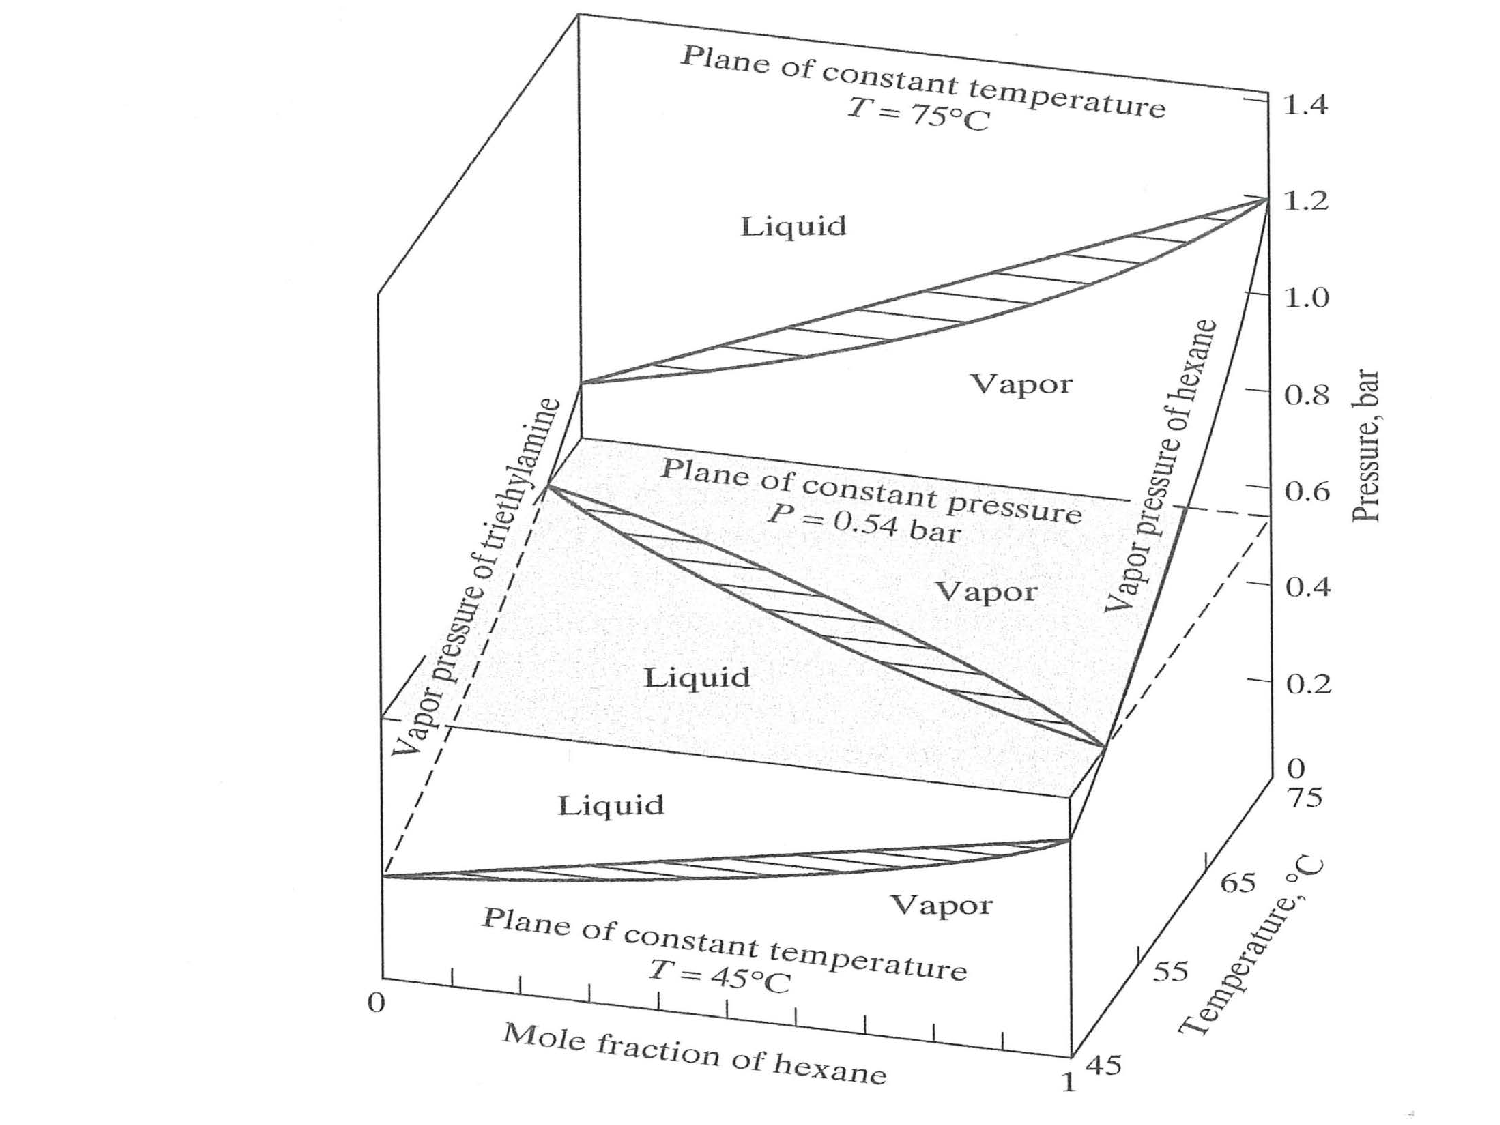
\includegraphics[width=.9\columnwidth,clip]{./../Pics/PTxy_diagram}
           \vspace{-.1cm}\caption{$P-T-xy$ diagram for hexane and triethylamine (extracted from Sandler, 2006).}\label{Mod04Fig01}
         \end{center}
       \end{figure}

In Fig.~\ref{Mod04Fig02}, a generic $P-T-xy$ diagram is shown. Vertical planes parallel to \blue{0-1-R-M-U-0} (\eg plane \blue{E-A-B-D-E}) indicates $P-xy$ diagrams at constant temperature, whereas horizontal planes parallel to \blue{K-J-I-H-K} indicates $T-xy$ diagrams at constant pressure. The (subcooled) liquid region lies \underline{above} the upper surface of the solid (grey) projection, and (superheated) vapour region lies \underline{below} the under surface. The interior of the solid projection between the two surfaces is the region of coexistence of both liquid and vapor phases. 

The $x_{1},y_{1}$ axis is limited to \blue{zero} and \blue{one}, thus at $x_{1}$ (or $y_{1}$) equal to zero, $x_{2}$ (or $y_{2}$) is equal to unity, \ie there is just pure component \blue{2} in solution. Similarly at $x_{1}$ (or $y_{1}$) equal to one, $x_{2}$ (or $y_{2}$) is equal to zero, \ie there is just pure component \blue{1} in solution. The diagram also depicts points \blue{$C_{1}$} and \blue{$C_{2}$} along the vertical planes of $x_{1},y_{1}=0$ and $x_{1},y_{1}=1$, respectively, these two points are the coordinates of the critical conditions $\left(P_{c,1}, P_{c,2}, T_{c,1} \text{ and } T_{c,2}\right)$ of both \underline{pure components}. Critical coordinates for mixtures at various compositions of \blue{1} and \blue{2} lie along a line on the rounded edge of the surface between \blue{$C_{1}$} and \blue{$C_{2}$}.
      \begin{figure}[h] 
         \begin{center}
             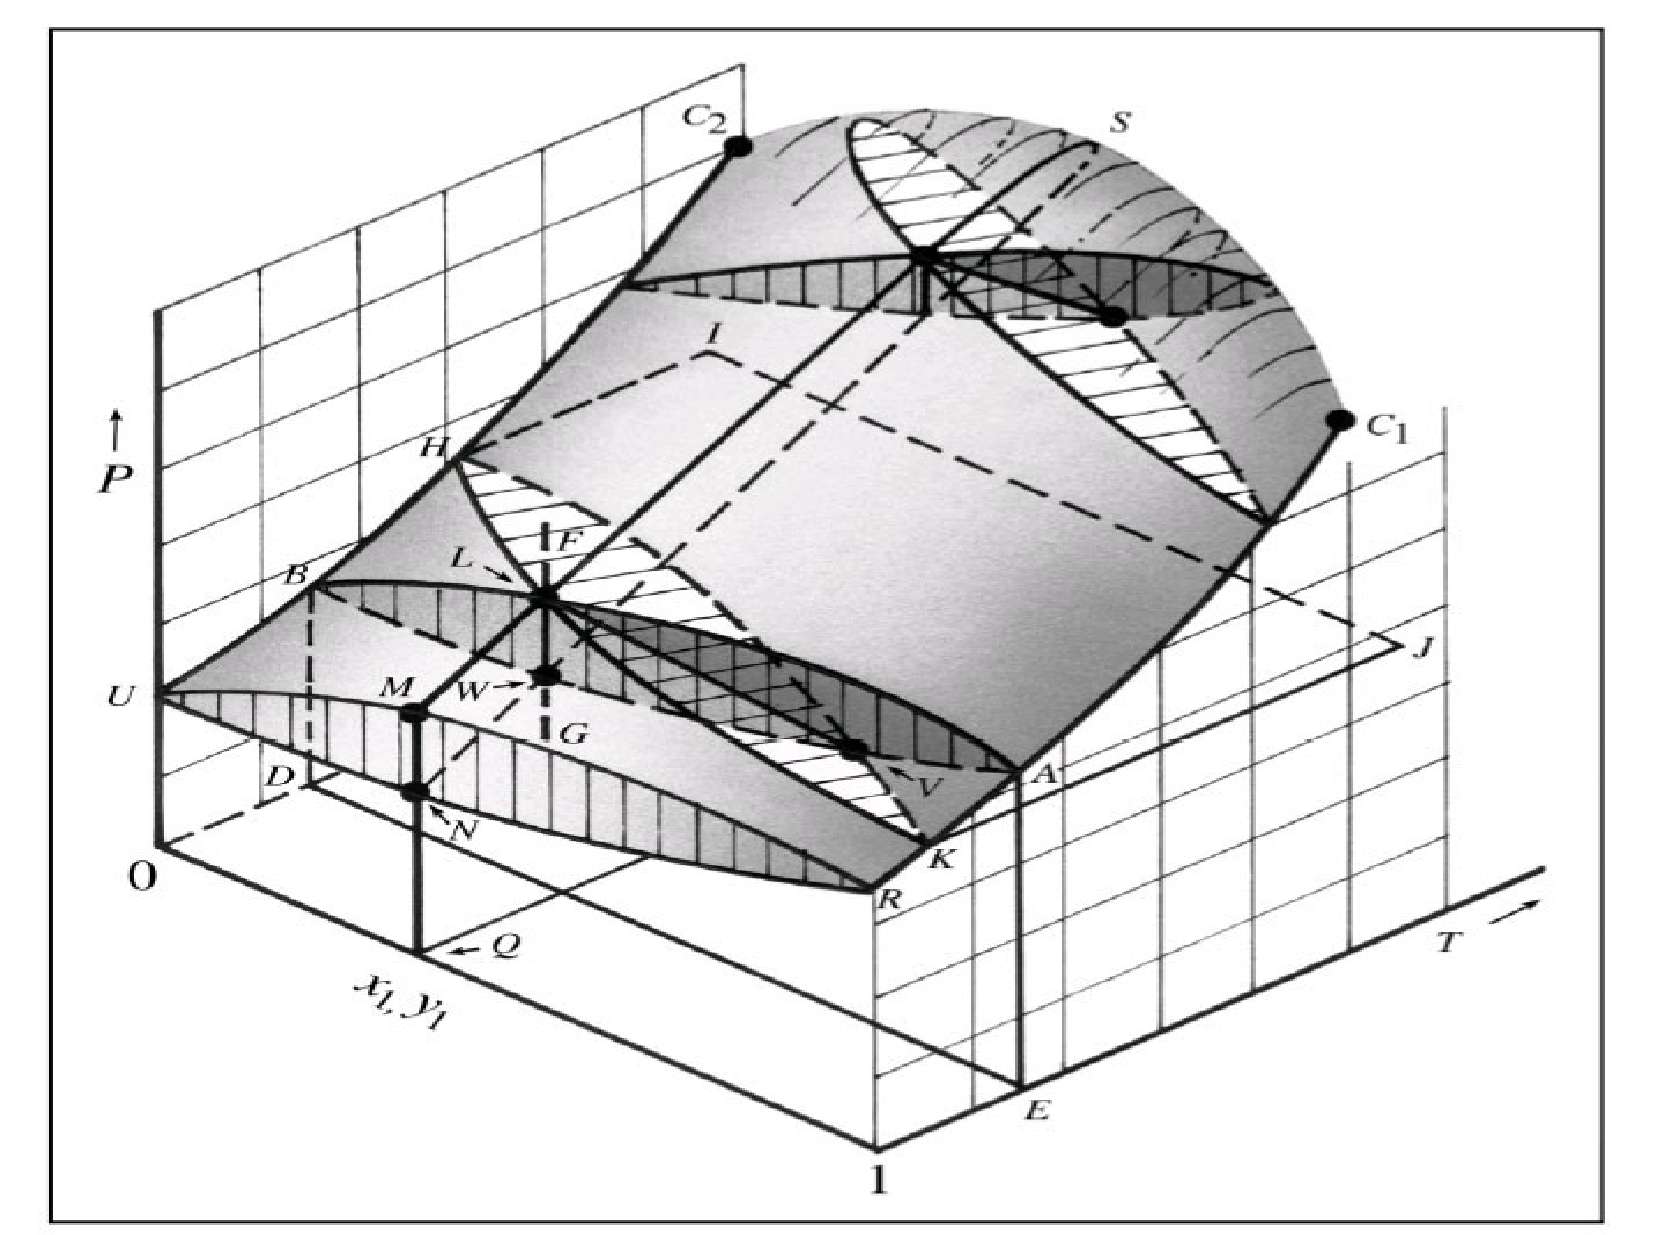
\includegraphics[width=.75\columnwidth,clip]{./Figs/PTxy_Digram} 
             \vspace{-.1cm}\caption{$P-T-xy$ diagram for binary mixtures (extracted from Smith, Van Ness and Abbott, 2000).}\label{Mod04Fig02}
         \end{center}
       \end{figure}
For each constant temperature plane, the upper line of the solid (grey) projection is the \blue{saturated liquid line} whilst the lower line is the \blue{saturated vapour line} (the reader should remember that these lines are also present for pure substances in the $Ts$ and $Ph$ diagrams , Fig.~\ref{Mod03Fig02}).

Compositions of each phase can be obtained from a parallel line linking $x_{1}$ and $y_{1}$. For example, in the `lens' \blue{U-M-R-N-U} contained in the plane \blue{0-U-M-R-1-Q-0}, the vapour phase $\left(\text{with composition }\red{y_{1}=\alpha}\text{ at } \blue{K_{1}}\right)$ is in equilibrium with the liquid phase $\left(\text{with composition }\red{x_{1}=\beta}\text{ at } \blue{K_{2}}\right)$. This parallel line, \blue{$K_{1}-K_{2}$}, is called \underline{tie-line} (Fig.~\ref{Mod04Fig03}b). The intersection of the tie-line with the saturated liquid line is referred as \blue{bubble pressure}, and the intersection with the saturated vapour line is called \blue{dew pressure} (at constant temperature).

$P-T-xy$ diagram, although insightful, is not very practical. Projections of $P-xy$ plane at constant temperature are shown in Fig.~\ref{Mod04Fig03}. Now, let's assume that the fluid of this diagram, Fig.~\ref{Mod04Fig03}(c), is at liquid phase at coordinate \blue{$M$} with composition \blue{$\left(x_{1}=x_{z};y_{1}=0\right)$}. As pressure is reduced along the \blue{$M-S$} line, the first bubble of vapour appears at \blue{$N$}; composition at this coordinate is \blue{$\left(x_{1}=x_{z};y_{1}=y_{BP}\right)$}, and this is called \blue{\it bubble point}. Further reduction of pressure to coordinate \blue{$Q$} (still at constant temperature), the fluid becomes partially vaporised and the composition at this coordinate is given by the {\it tie-line} \blue{$Q_{L}-Q_{V}$} -- \blue{$\left(x_{1}=x_{Q};,y_{1}=y_{Q}\right)$}. 
      \begin{figure}[h]
        \vbox{\hbox{\hspace{-1.cm}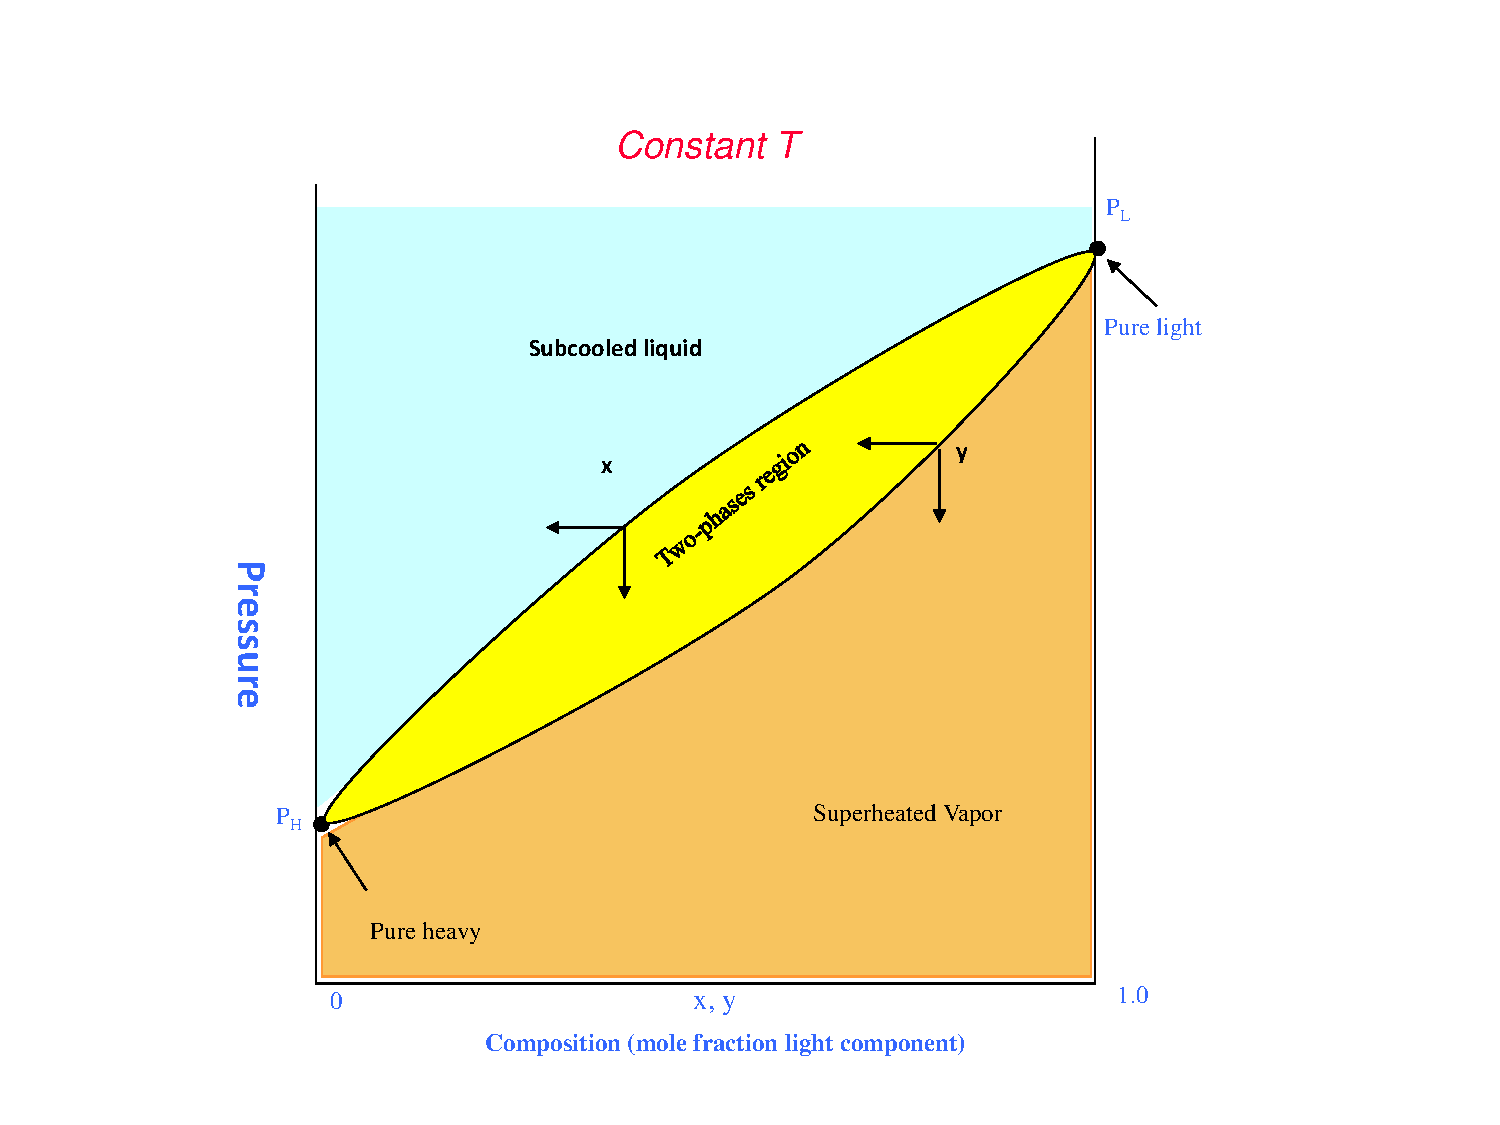
\includegraphics[width=.7\linewidth,clip]{./../Pics/VLE_Pxy_Diagram1}
            \hspace{-4.cm}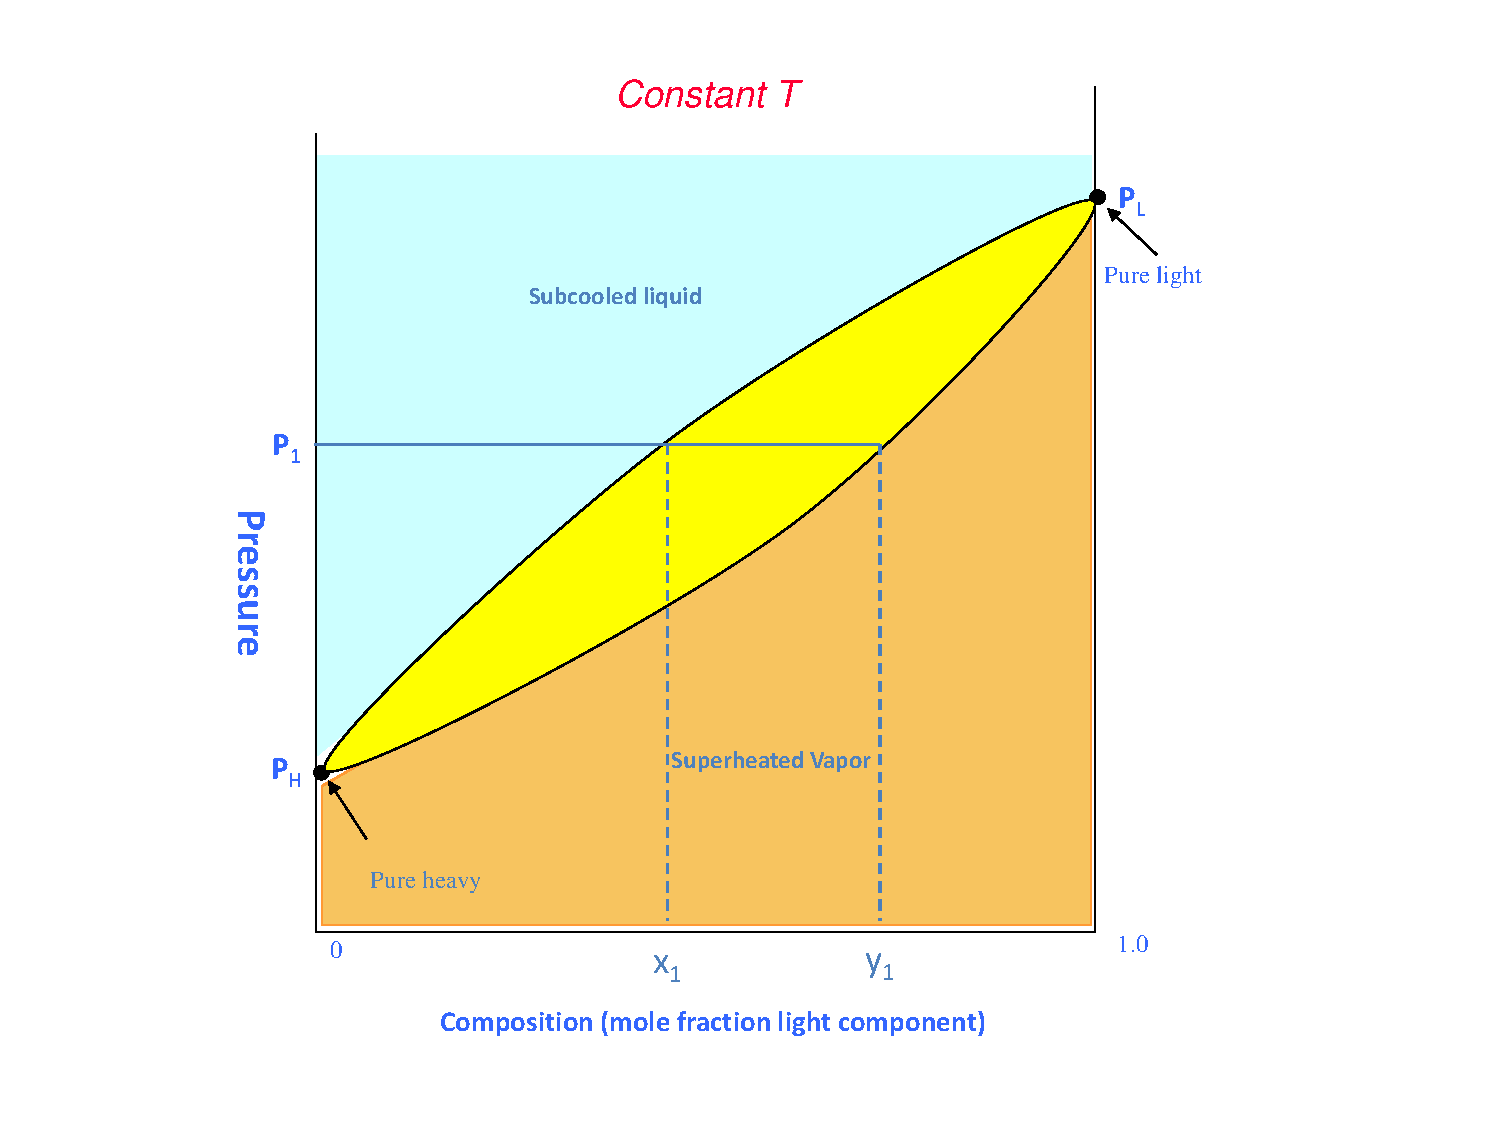
\includegraphics[width=.7\linewidth,clip]{./../Pics/VLE_Pxy_Diagram2}}
          \vspace{-.5cm}
          \hbox{\hspace{4.5cm}(a)\hspace{7cm}(b)}
          \vspace{-.5cm}\hbox{\hspace{3.cm}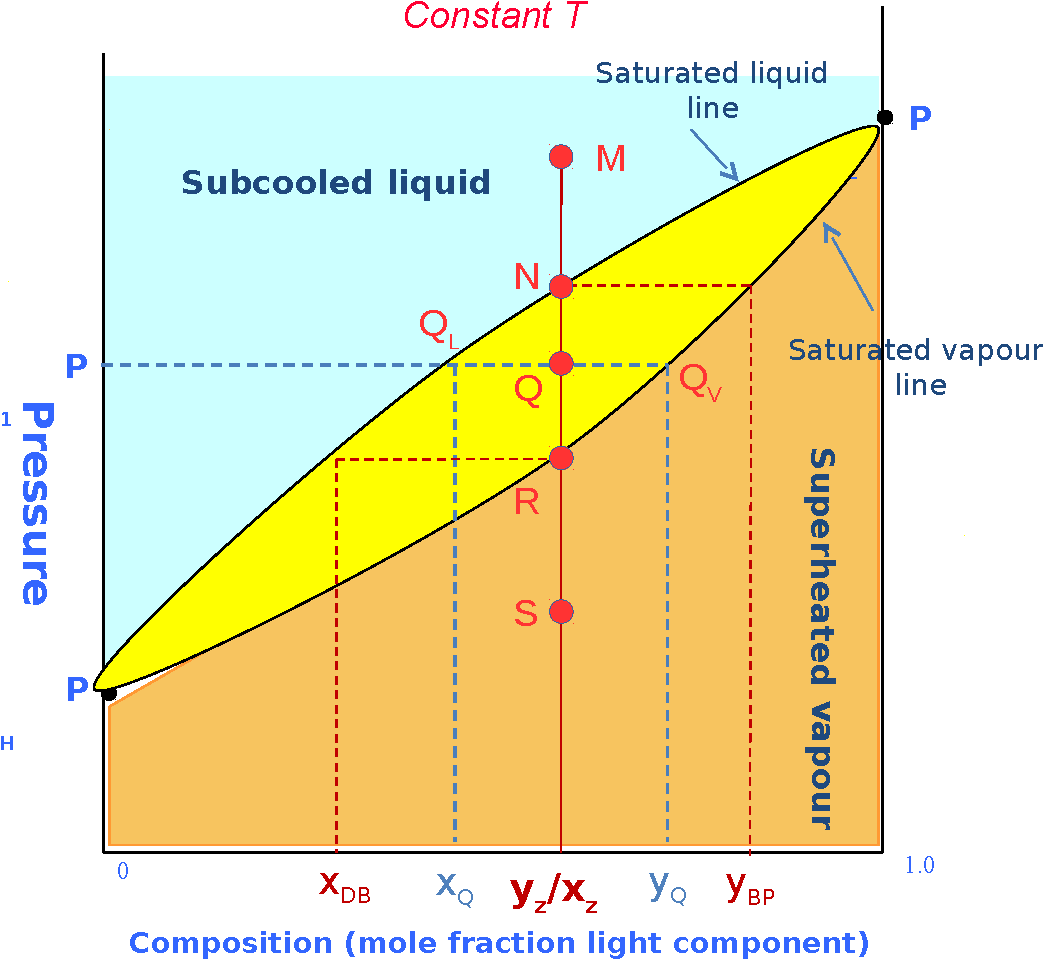
\includegraphics[width=.6\linewidth,clip]{./../Pics/VLE_Pxy_Diagram3b}}
          \vspace{-.1cm}
          \hbox{\hspace{7.5cm}(c)}}
             \vspace{-.1cm}\caption{VLE for binary mixtures: $P-xy$ diagrams at constant temperature.}\label{Mod04Fig03}
      \end{figure}
      
As the pressure is continuously reduced along line \blue{$Q-R$}, more liquid is vaporised until \blue{$R$}, when the last droplet of liquid (dew) is vaporised. This coordinate is called \blue{\it dew point}. The composition at $N$ is \blue{$\left(x_{1}=x_{DB};y_{1}=y_{z}\right)$}. Continued reduction of pressure towards \blue{$S$} leads to (pure) vapour region with composition \blue{$\left(x_{1}=0,y_{1}=y_{z}\right)$}.
     \begin{figure}[h]
        \vbox{\hbox{\hspace{3.cm}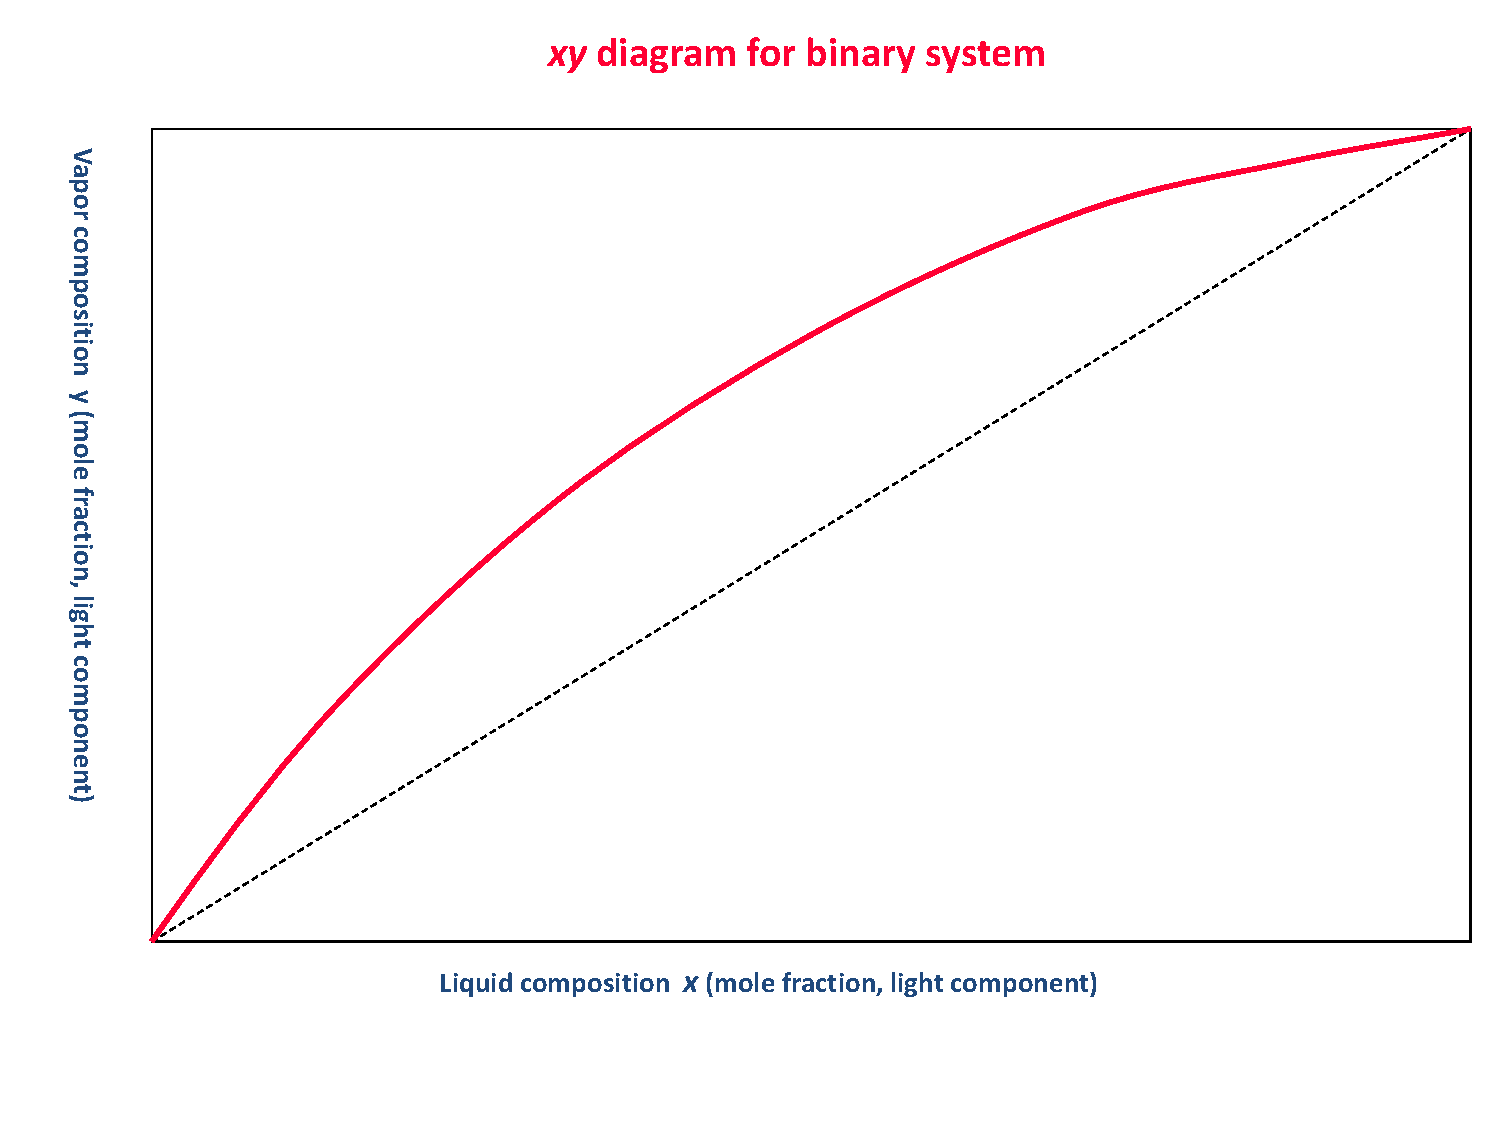
\includegraphics[width=.6\linewidth,clip]{./../Pics/VLE_xy_DiagramIdeal}}
          \vspace{-.5cm}
          \hbox{\hspace{8.cm}(a)}
          \hbox{\hspace{-1.cm}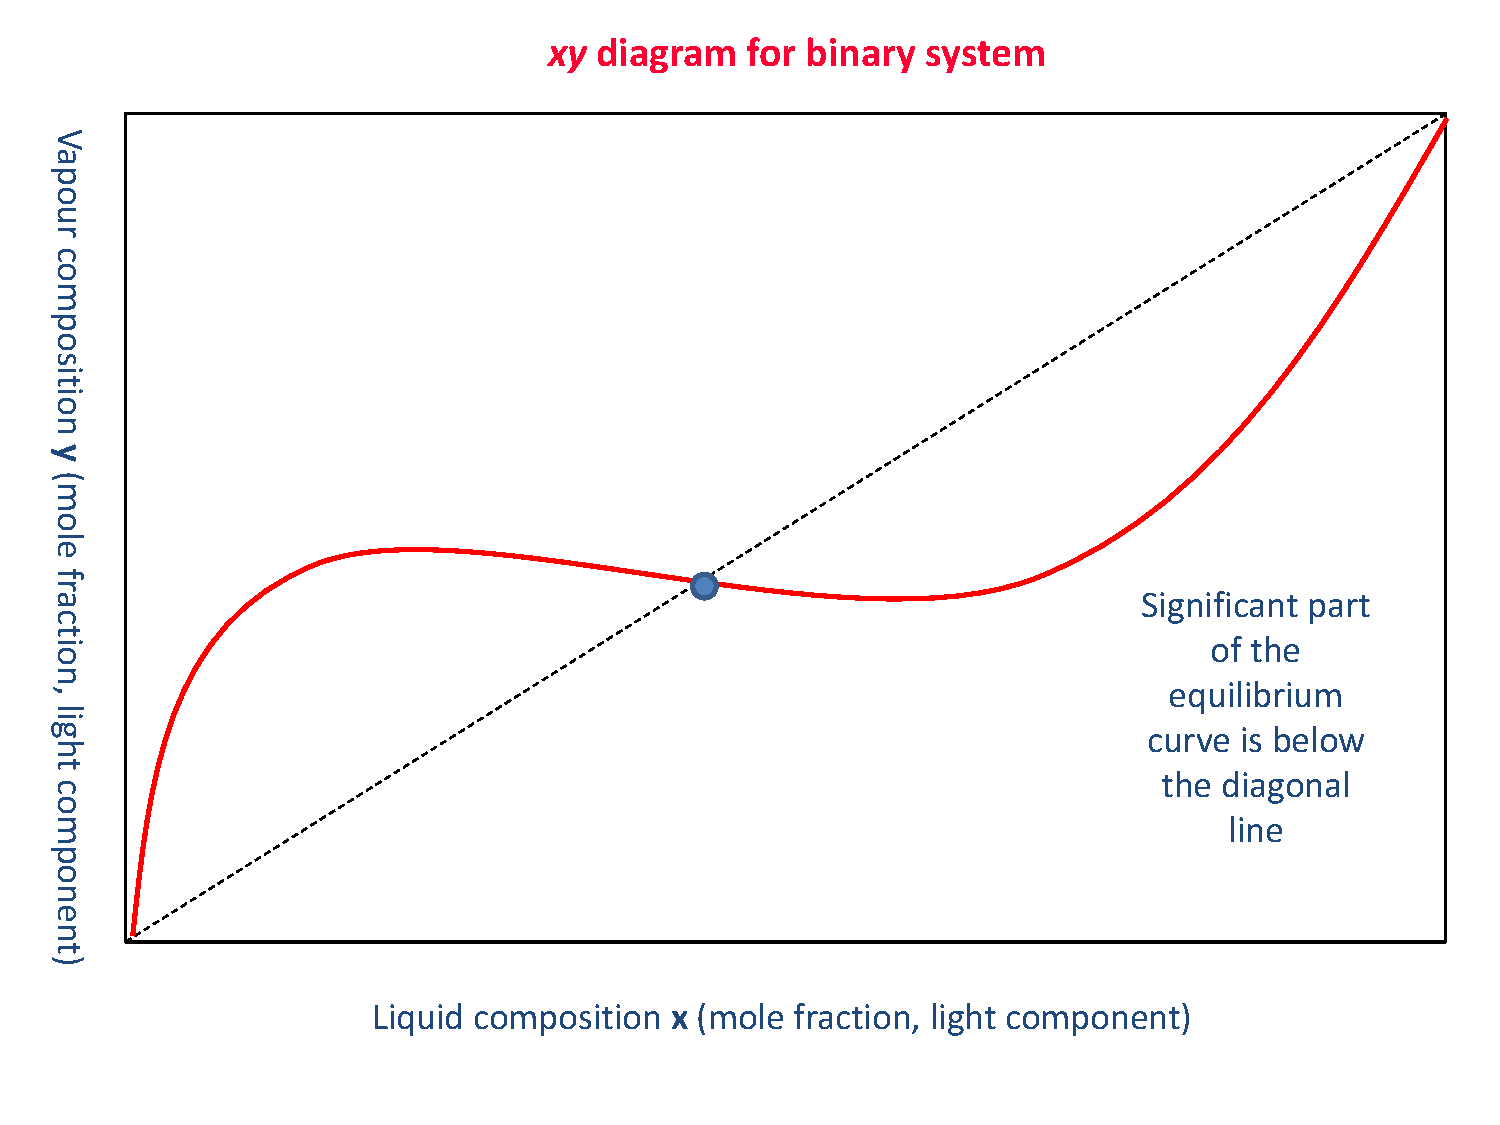
\includegraphics[width=.5\linewidth,clip]{./../Pics/VLE_xy_DiagramNonIdeal1}
            \hspace{-0.cm}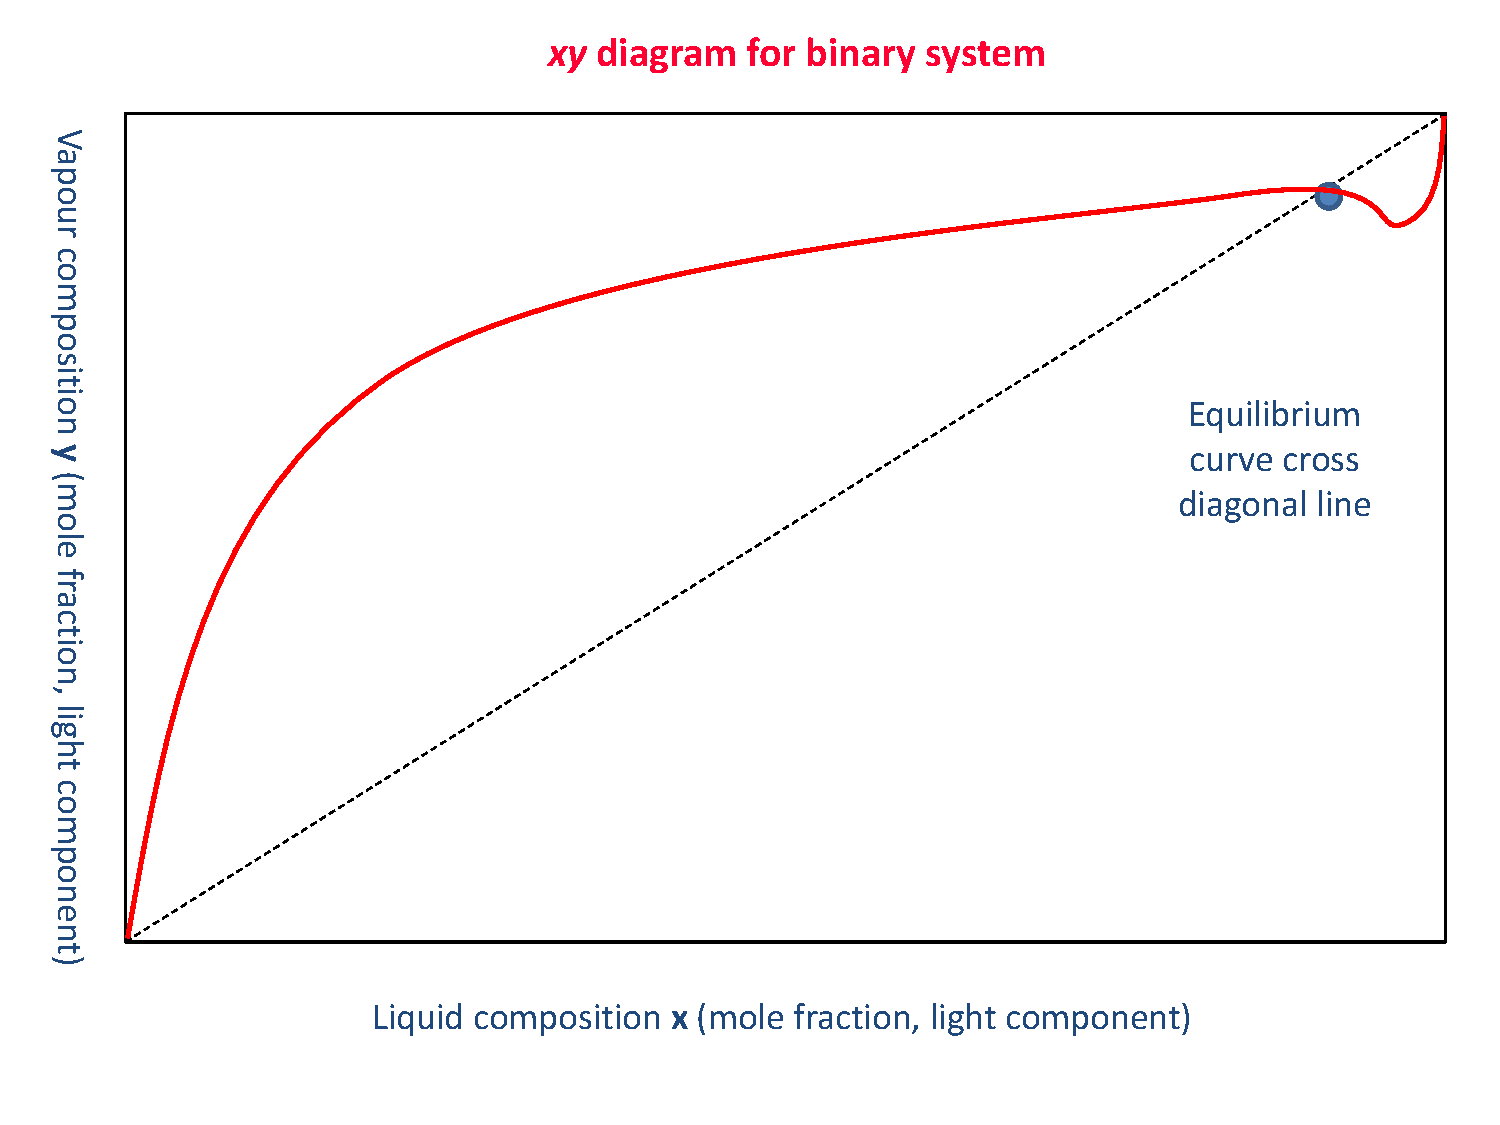
\includegraphics[width=.5\linewidth,clip]{./../Pics/VLE_xy_DiagramNonIdeal2}}
          \vspace{-.5cm}
          \hbox{\hspace{3.5cm}(b)\hspace{7.5cm}(c)}}
          \vspace{-.1cm}\caption{VLE for binary mixtures: $xy$ diagrams at constant pressure of (a) ideal and (b-c) non-ideal solutions.}\label{Mod04Fig04}
      \end{figure}

     Another common phase diagram is the $x-y$, Fig.~\ref{Mod04Fig04}(a), in which either pressure or temperature is kept constant. In this diagram, at constant pressure, there are two curves, the upper curve represents the composition at equilibrium with varying temperature. The straight line represents the equimolar composition, \ie $x_{1}=y_{1}$. However, in several solutions of industrial interest, molecular attractive forces from the heavier component (2) keep molecules of the more volatile component in the liquid solution, constraining its evaporation. This leads into an equilibrium pressure smaller than the expected at the same liquid composition. Such deviation from ideality is called \blue{\it azeotropy}. In practical terms, any component from solutions can often be separated through distillation processes, however azeotropes may lead to vapour-liquid-liquid equilibrium (VLLE) and other separations strategies may need to be used.  
     
%%% SUBSUBSECTION
\subsubsection{VLE Models: Raoult's Law}\label{Section:04:RaoultsLaw}
  \begin{subequations}
      The diagrams of binary (as well as multi-component) mixtures shown in the previous section are obtained from experiments and introduce a qualitative analysis of the PVT behaviour of solutions. However, classic thermodynamics provides a mathematical framework for systematic correlation, extension, generalisation and interpretation of data.
      For ideal vapour-liquid systems, the \blue{Raoult's law} provides a relation between the compositions of the vapour and liquid phases,
         \begin{shaded}
           \begin{equation}
             P_{i} = y_{i}P = x_{i}P_{i}^{\text{sat}},\;\;\;\forall i\in\left\{1,2,\cdots,\mathcal{C}\right\}\label{Mod04_RaoultLaw} 
           \end{equation}
         \end{shaded}
      $P_{i}=y_{i}P$ in Eqn.~\ref{Mod04_RaoultLaw} is known as \blue{\it partial pressure}, and $P_{i}^{\text{sat}}$ is the saturated pressure (or saturated vapour pressure) of pure species $i$ and was defined in Eqn.~\ref{Mod03_Antoine}. This rather simple relation can only be applied to ideal solutions (for both phases). For a gas mixture to be considered ideal the pressure need to be equal or smaller than atmospheric. There are several relations for ideal gas mixtures, \eg
       \begin{enumerate}[a)]
           \begin{shaded}    
               \item Dalton's Law:
                  \begin{equation}
                      P = \summation[P_{i}]{i=1}{\mathcal{C}} = \summation[y_{i}P]{i=1}{\mathcal{C}}\label{Mod04_DaltonLaw}
                  \end{equation}
           \end{shaded}
           \item Amagat's Law:
              \begin{displaymath}
                  V^{\text{t}} = \summation[V_{i}^{\text{t}}]{i=1}{\mathcal{C}} = \summation[y_{i}V^{\text{t}}]{i=1}{\mathcal{C}}
              \end{displaymath}
           \item Kay's rule for pseudo-critical temperature and pressure:
              \begin{displaymath}
                  T_{c}^{\text{t}} = \summation[y_{i}T_{c,i}]{i=1}{\mathcal{C}},\;\;\text{ and }\;\;P_{c}^{\text{t}} = \summation[y_{i}P_{c,i}]{i=1}{\mathcal{C}}
              \end{displaymath}
       \end{enumerate}
       Liquid solutions are considered ideals if the molecular interaction between the similar species is identical to that between dissimilar species. Thermodynamics of liquid solutions are the focus of Module~\ref{Section:05}.
       
\end{subequations}

%%% SUBSUBSECTION
\subsubsection{Henry's Law}\label{Section:04:HenryLaw}

A typical application of VLE is when gases are solubilised in liquid solutions, \eg O$_{2}$ in water, CO$_{2}$ in soft drinks, air in the blood stream etc. In these cases, gases have relatively low solubility (mole fraction varying between 10$^{-5}$ to 10$^{-2}$) in liquid solvents. Application of Raoult's law is limited to $P^{\text{sat}}$. If the temperature exceeds the critical temperature, Raoult's law is no longer applicable as $P^{\text{sat}}$ can not be defined. For such cases, a new relation is required that relates compositions in both phases and the pressure,
\begin{shaded}
  \begin{equation}
      P_{i} = y_{i}P = x_{i}\mathcal{H}_{i},\label{Mod04_HenryLaw} 
  \end{equation}
\end{shaded}
\noindent where $\mathcal{H}$ is the Henry's constant obtained experimentally. Values of Henty's contant for several gases dissolved in water at 25$^{\circ}$C is shown in Table~\ref{Mod04_HenryLawTable}
 \begin{table}
  \begin{center}
    \begin{tabular}{l r || l r }
      \hline
       {\bf Gas}    &  ${\bf \mathcal{H}\text{ (bar)}}$ & {\bf Gas}    &  ${\bf \mathcal{H}\text{ (bar)}}$ \\
      \hline
         Acetylene  &   1350                            & He           &  126600 \\
         Air        &   72950                           & H$_{2}$      &  71600  \\
         CO$_{2}$    & 1670                              & H$_{2}$S     & 550 \\
         CO         &  54600                            &  CH$_{4}$    &  41850 \\
         C$_{2}$H$_{6}$ & 30600                          &  N$_{2}$     & 87650  \\
         Ethylene  & 11550                              & O$_{2}$      & 44380 \\
      \hline
    \end{tabular}
    \caption{Henry's constant for gases dissolved in water at 25$^{\circ}$C.}\label{Mod04_HenryLawTable}
  \end{center}
\end{table}

  
%%% SUBSECTION
\subsection{Industrial Applications: Multi-Component VLE}

%%% SUBSUBSECTION
\subsubsection{Dew-point and Bubble-point Calculations using Raoult’s Law }

Let's consider a vapour-liquid system containing $\mathcal{C}$ chemical species. From the phase rule the number of degrees of freedom is $\mathcal{C}$ that are $T$, $P$, $x_{i}$ and/or $y_{i}$. Four types of problems are possible:
\begin{center}
   \begin{tabular}{|l c c|}
      \hline 
      $\mathbf{VLE}$ {\bf Problem} & {\bf Specified Variables} &  {\bf Computed Variables} \\  
      \hline
          {\bf Bubble Pressure}        &  $T$ and $x_{i}$           &   $P$ and $y_{i}$          \\
          {\bf Dew Pressure}           &  $T$ and $y_{i}$           &   $P$ and $x_{i}$          \\
          {\bf Bubble Temperature}     &  $P$ and $x_{i}$           &   $T$ and $y_{i}$          \\
          {\bf Dew Temperature}        &  $P$ and $y_{i}$           &   $T$ and $x_{i}$          \\     
      \hline
   \end{tabular}
\end{center}
Such problems are calculated using three relations:
\begin{displaymath}
    P_{i} = y_{i}P = x_{i}P_{i}^{\text{sat}}, \;\;\; \summation[x_{i}]{i=1}{\mathcal{C}} = 1, \;\;\text{ and }\;\; \summation[y_{i}]{i=1}{\mathcal{C}} = 1,
\end{displaymath}
bearing in mind that $P_{i}^{\text{sat}}$ is expressed as a function of $T$. Thus,
\begin{enumerate}[a)]
    \item Bubble pressure: Given $T$ and $x_{i}$ $\left(\text{with }i=1,\cdots,\mathcal{C}\right)$, find $P$ that solves,
        \begin{displaymath}
           \summation[y_{i}]{i=1}{\mathcal{C}} = 1 \;\;\Longrightarrow\;\; \summation[\frc{x_{i}P_{i}^{\text{sat}}}{P}]{i=1}{\mathcal{C}} = 1,
        \end{displaymath}
        and then calculate $y_{i}= \frc{x_{i}P_{i}^{\text{sat}}}{P}$.
        
    \item Bubble temperature: Given $P$ and $x_{i}$ $\left(\text{with }i=1,\cdots,\mathcal{C}\right)$, find $T$ that solves,
        \begin{displaymath}
           \summation[y_{i}]{i=1}{\mathcal{C}} = 1 \;\;\Longrightarrow\;\; \summation[\frc{x_{i}P_{i}^{\text{sat}}}{P}]{i=1}{\mathcal{C}} = 1,
        \end{displaymath}
        and then calculate $y_{i}= \frc{x_{i}P_{i}^{\text{sat}}}{P}$.
      
    \item Dew pressure: Given $T$ and $y_{i}$ $\left(\text{with }i=1,\cdots,\mathcal{C}\right)$, find $P$ that solves,
        \begin{displaymath}
           \summation[x_{i}]{i=1}{\mathcal{C}} = 1 \;\;\Longrightarrow\;\; \summation[\frc{y_{i}P}{P_{i}^{\text{sat}}}]{i=1}{\mathcal{C}} = 1,
        \end{displaymath}
        and then calculate $y_{i}= \frc{x_{i}P_{i}^{\text{sat}}}{P}$.
      
    \item Dew temperature: Given $P$ and $y_{i}$ $\left(\text{with }i=1,\cdots,\mathcal{C}\right)$, find $T$ that solves,
        \begin{displaymath}
           \summation[x_{i}]{i=1}{\mathcal{C}} = 1 \;\;\Longrightarrow\;\; \summation[\frc{y_{i}P}{P_{i}^{\text{sat}}}]{i=1}{\mathcal{C}} = 1,
        \end{displaymath}
        and then calculate $y_{i}= \frc{x_{i}P_{i}^{\text{sat}}}{P}$.
\end{enumerate}


%%% SUBSUBSECTION
\subsubsection{K-Value Correlations for Hydrocarbon Systems}

As discussed in Modules~\ref{Section:02}-~\ref{Section:03}, cubic equations of state are often used to describe the PVT behaviour of vapour and liquid phases of pure chemical species and mixtures. Although the use of cubic EOS is widely spread over the chemical industry, applicability to liquid phase is still limited. Several alternatives have been proposed and developed over the past 50 years, one of them, mostly used in petroleum and petrochemical industry for hydrocarbons, is called {\it K-value correlation}. $K$ is defined as
\begin{shaded}
   \begin{equation}
      K_{i} = \frc{P_{i}^{\text{sat}}}{P} = \frc{y_{i}}{x_{i}}.\label{Mod04_KValue}
   \end{equation}
\end{shaded}
Values for $K_{i}$ are tabulated for a large number of hydrocarbons at several pressure and temperature conditions and can be found in any chemical engineering handbook as part of \blue{DePriester chart} (Fig.~\ref{Mod04Fig05}).
  \begin{figure}[h]
     \begin{center}
         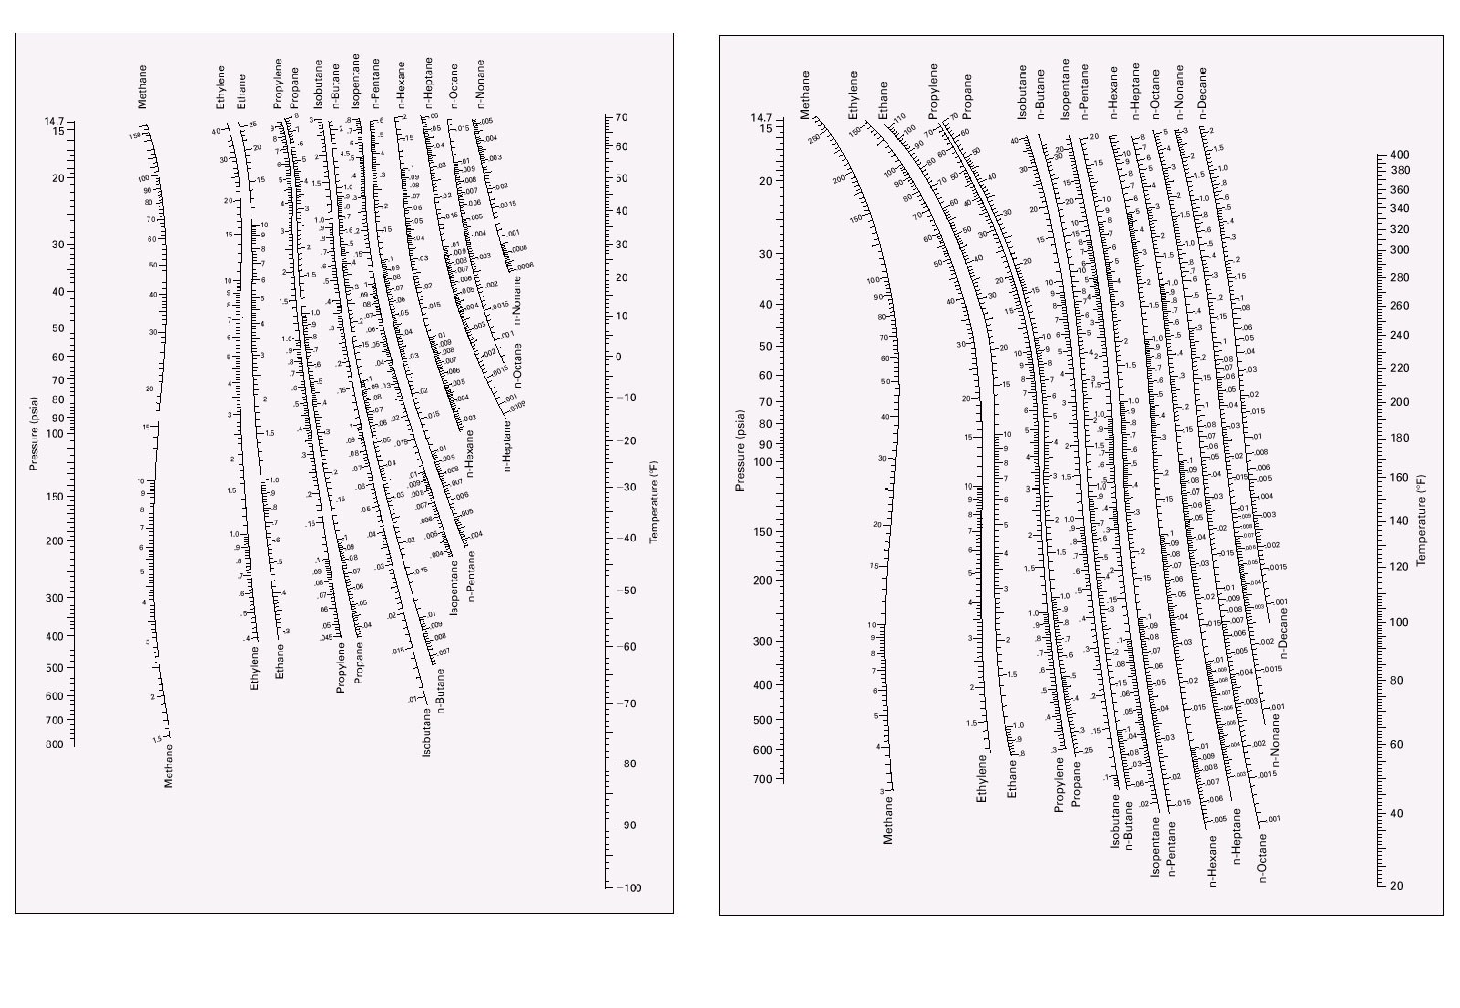
\includegraphics[width=1.\linewidth,clip]{./Figs/DePriesterCharts}
     \end{center}
     \caption{DePriester chart for several hydrocarbons (extracted from Smith, Van Ness and Abbott, 2000).}\label{Mod04Fig05}
  \end{figure}


%%% SUBSUBSECTION
\subsubsection{Flash Distillation}

Flash distillation is a common process in chemical industry to obtain solutions with the required enrichment from a feed-stock. Figure~\ref{Mod04Fig06} shows a schematic of this process, where a liquid stream (\ie with pressure equal to or larger than its bubble point pressure) with molar fraction $F$ and overall composition $z_{i}$ is injected into a separation vessel through a pressure reduction valve. The sudden reduction in pressure leads to partial evaporation (\ie {\it flash}) of the liquid feed resulting in the formation of a vapour and a liquid stream. Vapour and Liquid streams have molar fraction $V$ and $L$, respectively, with compositions of $y_{i}$ and $x_{i}$. 
  \begin{figure}[h]
     \begin{center}
         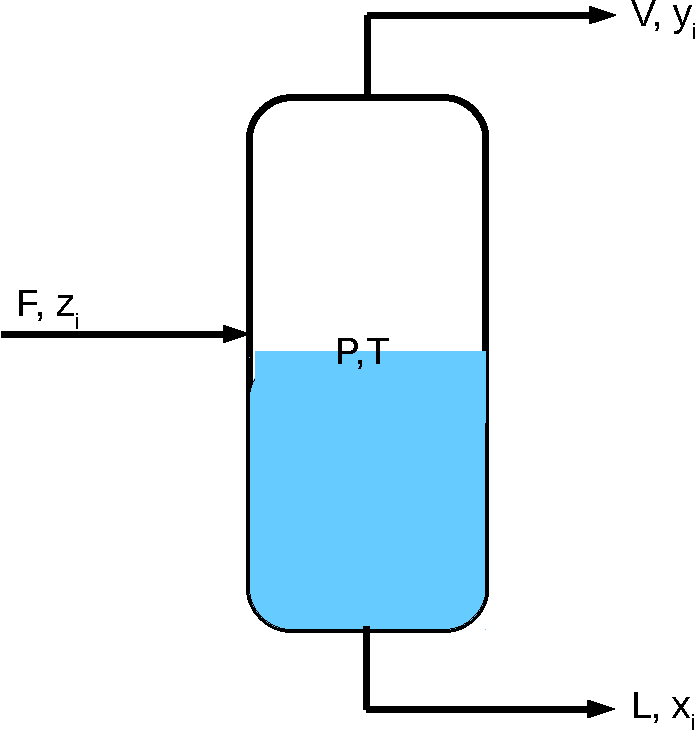
\includegraphics[width=.7\linewidth,clip]{./Figs/FlashDistillation}
     \end{center}
     \caption{Schematic of a flash distillation process.}\label{Mod04Fig06}
  \end{figure}
        
      The overall mass balance of the system is
         \begin{displaymath}
             F = V + L,
         \end{displaymath}
         for convenience, $F$ is assumed equal to unity, $F=1$. Similarly, the mass balance for each component $i$ is
         \begin{displaymath}
            z_{i} = x_{i}L + y_{i}V = x_{i}\left(1-V\right) + y_{i}V.
         \end{displaymath}
         Replacing $x_{i} = \frc{y_{i}}{K_{i}}$,
         \begin{displaymath}
           z_{i} = \frc{y_{i}}{K_{i}}\left(1-V\right) + y_{i}V \;\;\Longrightarrow \;\;y_{i} = \frc{z_{i}K_{i}}{1+V\left(K_{1}-1\right)}. 
         \end{displaymath}
         As $\summation[y_{i}]{i=1}{\mathcal{C}} = 1$,
         \begin{shaded}
           \begin{equation}
              \summation[\frc{z_{i}K_{i}}{1+V\left(K_{i}-1\right)}]{i=1}{\mathcal{C}} = 1.\label{Mod04_FlashEquation} 
           \end{equation}
         \end{shaded}
         Solving a $P-T$ flash problem is to \underline{find $V$} that satisfies Eqn.~\ref{Mod04_FlashEquation}.
      
\clearpage

%%% SUBSECTION
\subsection{Examples}

\begin{enumerate}[1)] 
%%%
%%% EXAMPLE
%%%
   \item\label{Mod04Ex01} Assuming a mixture of n-pentane $\left(nC_{5}\right)$ and n-heptane $\left(nC_{7}\right)$ is ideal, draw vapour-liquid $x_{5}\times y_{5}$ and $P-x_{5}y_{5}$ equilibrium diagrams for this mixtures at constant temperature of 50$^{\circ}$C. Given $P^{\text{sat}}$ relation,
    \begin{displaymath}
      \ln{P_{i}^{\text{sat}}} = A_{i} - \frc{B_{i}}{RT}
    \end{displaymath}
    with $A_{nC_{5}}=10.422$, $A_{nC_{7}}=11.431$, $B_{nC_{5}}=26799 \text{ J.mol}^{-1}$ and $B_{nC_{7}}=35200 \text{ J.mol}^{-1}$. Also [$P$] = bar and [$T$] = K.

% SOLUTION
 \noindent{\bf Solution:} At $T=$50$^{\circ}$C = 323.15 K, vapour saturated pressures for $nC_{5}$ and $nC_{7}$ (for short notation, let's use 5 and 7 as $nC_{5}$ and $nC_{7}$, respectively) are
           \begin{displaymath}
              P_{5}^{\text{sat}} = 1.5639\text{ bar}\;\;\text{ and }\;\;P_{7}^{\text{sat}} = 0.1881\text{ bar}.
           \end{displaymath}
           In order to calculate the equilibrium pressure at each liquid $nC_{5}$ composition, $x_{5}$,
           \begin{eqnarray}
               && P_{i} = x_{i}P_{i}^{\text{sat}} \;\;\Longleftrightarrow \;\; P = \summation[P_{i}]{i=1}{\mathcal{C}} = \summation[x_{i}P_{i}^{\text{sat}}]{i=1}{\mathcal{C}} \nonumber \\
               && P = x_{5}P_{5}^{\text{sat}} + x_{7}P_{7}^{\text{sat}} = x_{5}P_{5}^{\text{sat}} + \left(1-x_{5}\right)P_{7}^{\text{sat}} \nonumber 
           \end{eqnarray}
           And for vapour composition (Raoult's law),
           \begin{displaymath}
               y_{i} P = x_{i}P_{i}^{\text{sat}}  \;\;\Longleftrightarrow \;\; y_{5} = \frc{x_{5}P_{5}^{\text{sat}}}{P},
           \end{displaymath}
           replacing pressure, $P$, from the previous equation
           \begin{displaymath}
               y_{5} = \frc{x_{5}P_{5}^{\text{sat}}}{x_{5}P_{5}^{\text{sat}} + \left(1-x_{5}\right)P_{7}^{\text{sat}}}.
           \end{displaymath}
           The $x_{5} \times y_{5}$ diagram may be plot by giving values to $0.0\leq x_{5} \leq 1.0$ and calculating $x_{5}$ through the equation above.

           The $P-x_{5}y_{5}$ diagram may be plot using the relations,
           \begin{displaymath}
               y_{5} = \frc{x_{5}P_{5}^{\text{sat}}}{P}\;\;\;\text{ and }\;\;\; P = x_{5}P_{5}^{\text{sat}} + \left(1-x_{5}\right)P_{7}^{\text{sat}} \;\Longrightarrow\; x_{5} = \frc{P-P_{7}^{\text{sat}}}{P_{5}^{\text{sat}}-P_{7}^{\text{sat}}}.
           \end{displaymath}
           Thus, given values for $P_{7}^{\text{sat}}\leq P \leq P_{5}^{\text{sat}}$ $\Rightarrow$ Calculate $x_{5}$  $\Rightarrow$ Calculate $y_{5}$.
           
      \begin{figure}[h]
         \vbox{
             \hbox{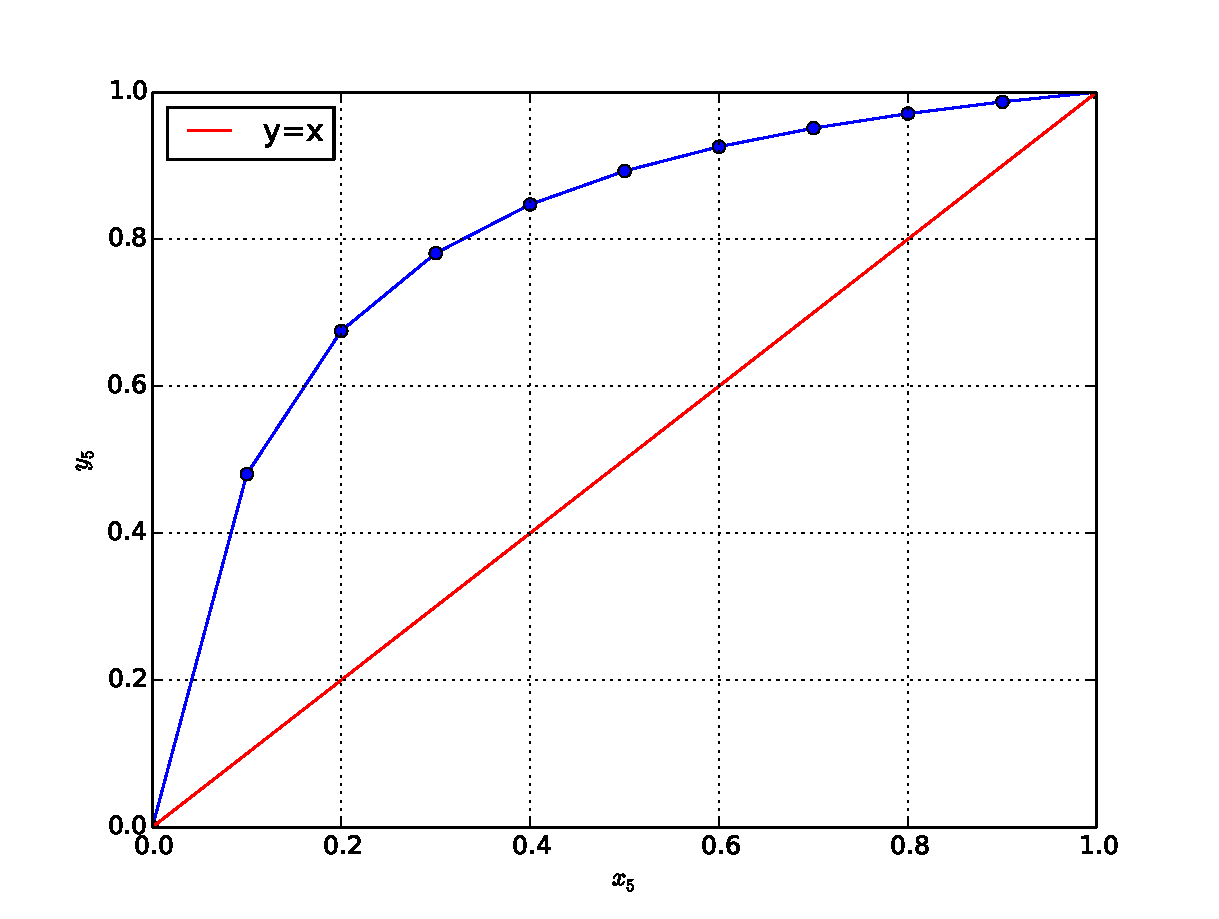
\includegraphics[width=.5\linewidth,clip]{./Figs/Mod4Ex1}
                   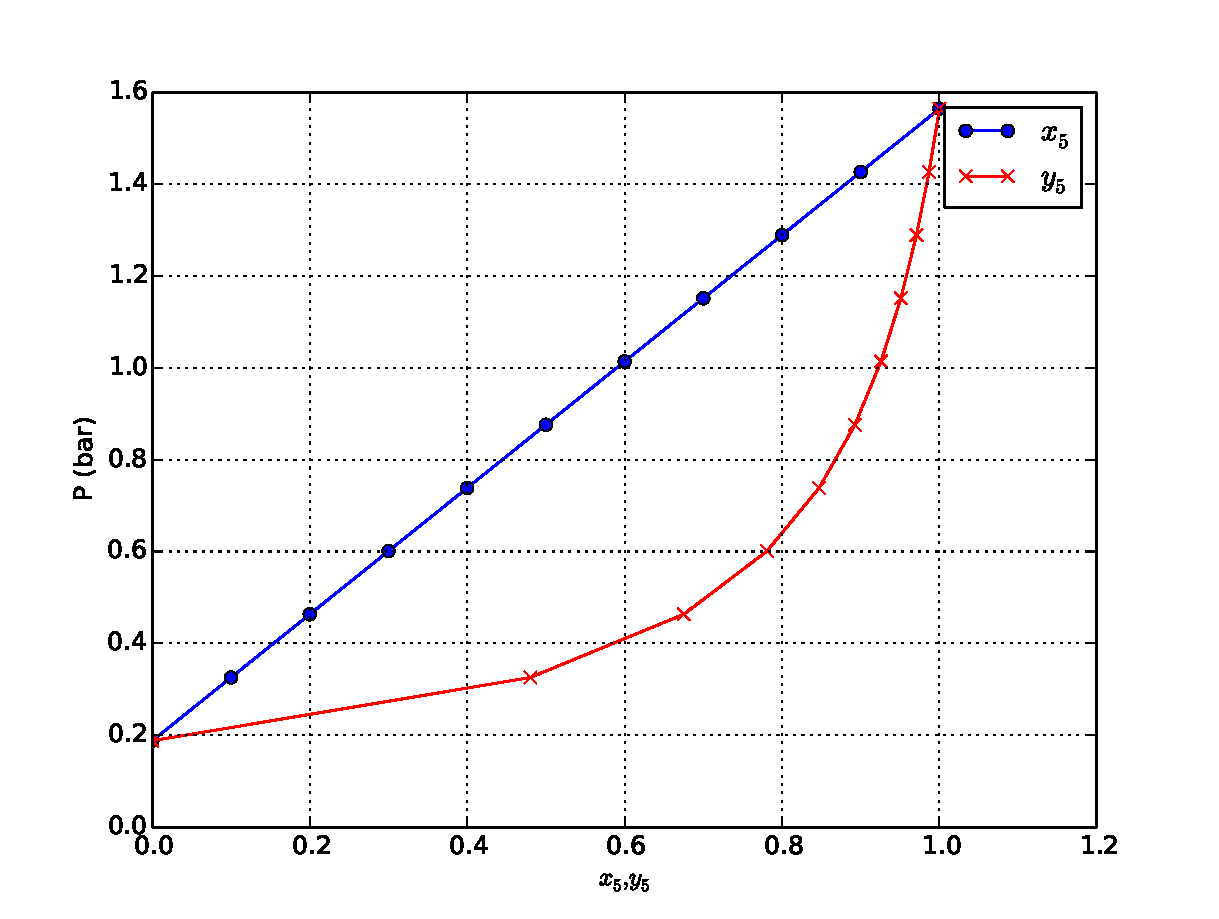
\includegraphics[width=.5\linewidth,clip]{./Figs/Mod4Ex1b}}}
         \caption{Example~\ref{Mod04Ex01}}
      \end{figure}
\clearpage
 % 
%%%
%%% EXAMPLE
%%%
   \item\label{Mod04Ex02} Assuming a mixture of n-pentane $\left(nC_{5}\right)$ and n-heptane $\left(nC_{7}\right)$ is ideal, draw vapour-liquid $x_{5}\times y_{5}$ and $T-x_{5}y_{5}$ equilibrium diagrams for this mixtures at constant pressure of 1.013 bar. Given $P^{\text{sat}}$ relation,
    \begin{displaymath}
      \ln{P_{i}^{\text{sat}}} = A_{i} - \frc{B_{i}}{RT}
    \end{displaymath}
    with $A_{nC_{5}}=10.422$, $A_{nC_{7}}=11.431$, $B_{nC_{5}}=26799 \text{ J.mol}^{-1}$ and $B_{nC_{7}}=35200 \text{ J.mol}^{-1}$. Also [$P$] = bar and [$T$] = K.

% SOLUTION
 \noindent{\bf Solution:} In this problem, equilibrium temperature and compositions are not known, thus
          \begin{displaymath}
              P = x_{5}P_{5}^{\text{sat}} + x_{7}P_{7}^{\text{sat}} = x_{5}P_{5}^{\text{sat}} + \left(1 - x_{5}\right)P_{7}^{\text{sat}} = 1.013\text{ bar},
          \end{displaymath}
          where $P_{i}^{\text{sat}}$ is non-linear function of the temperature $T$, \ie
          \begin{displaymath}
              P = x_{5}\exp{\left(A_{5} - \frc{B_{5}}{RT}\right)} + \left(1 - x_{5}\right)\exp{\left(A_{7} - \frc{B_{7}}{RT}\right)}.
          \end{displaymath}
          This equation has 2 unknowns, $x_{5}$ and $T$, however we know that $0.0\leq x_{5} \leq 1.0$, thus we can give values on this range $\Rightarrow$ calculate $T$  $\Rightarrow$  obtain $y_{5}$.
          \begin{center}
              \begin{tabular}{ c c c }
                  $\mathbf{x_{5}}$ & $\mathbf{T}${\bf(K)}  & $\mathbf{y_{5}}$ \\
                    0.0000          & 370.80                & 0.0000   \\
                    0.1000          & 357.80                & 0.4050   \\
                    0.2000          & 347.73                & 0.6249   \\
                    0.3000          & 339.73                & 0.7535   \\
                    0.4000          & 333.21                & 0.8345   \\
                    0.5000          & 327.77                & 0.8881   \\
                    0.6000          & 323.13                & 0.9257   \\
                    0.7000          & 319.12                & 0.9528   \\
                    0.8000          & 315.60                & 0.9728   \\
                    0.9000          & 312.47                & 0.9881   \\
                    1.0000          & 309.67                & 1.0000   
              \end{tabular}
           \end{center}
           
      \begin{figure}[h]
         \vbox{
             \hbox{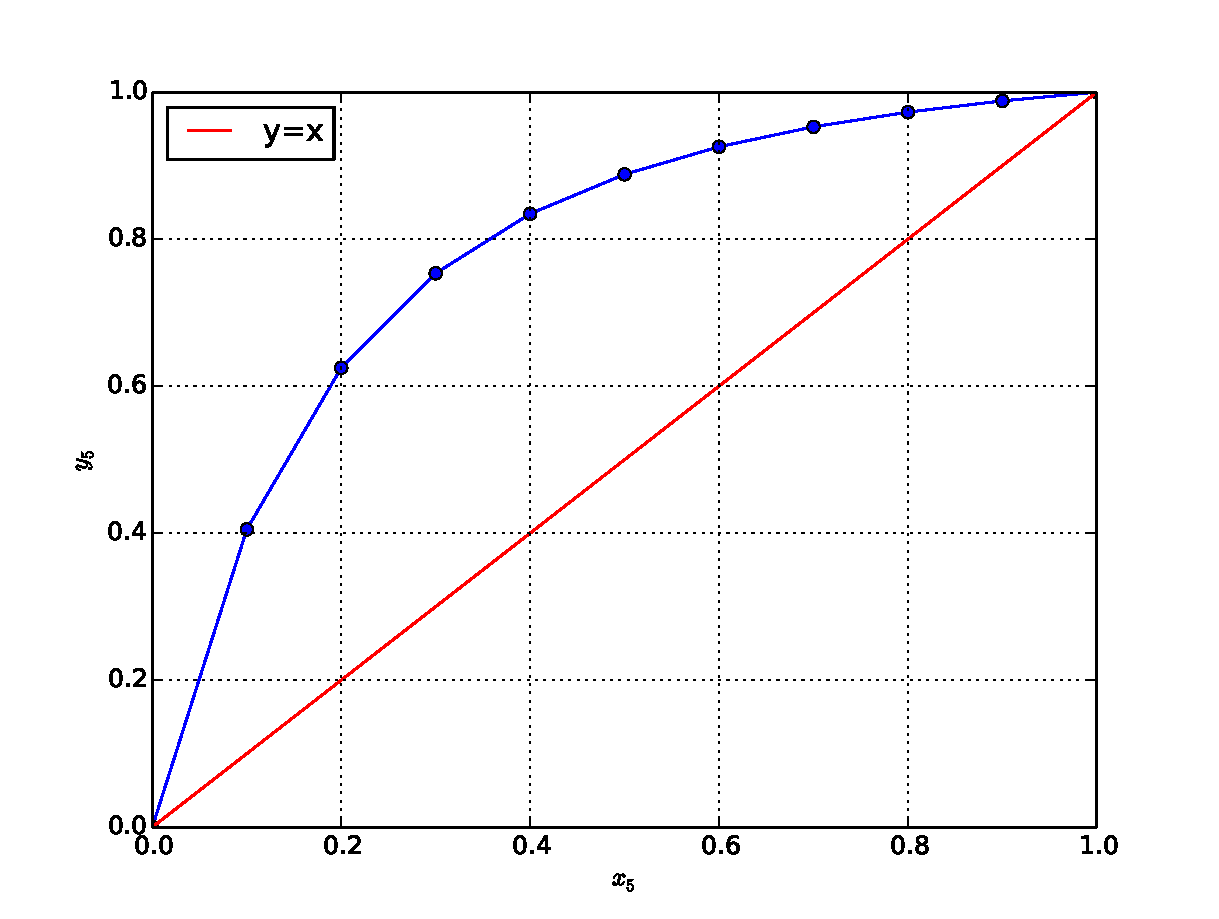
\includegraphics[width=.5\linewidth,clip]{./Figs/Mod4Ex2a}
                   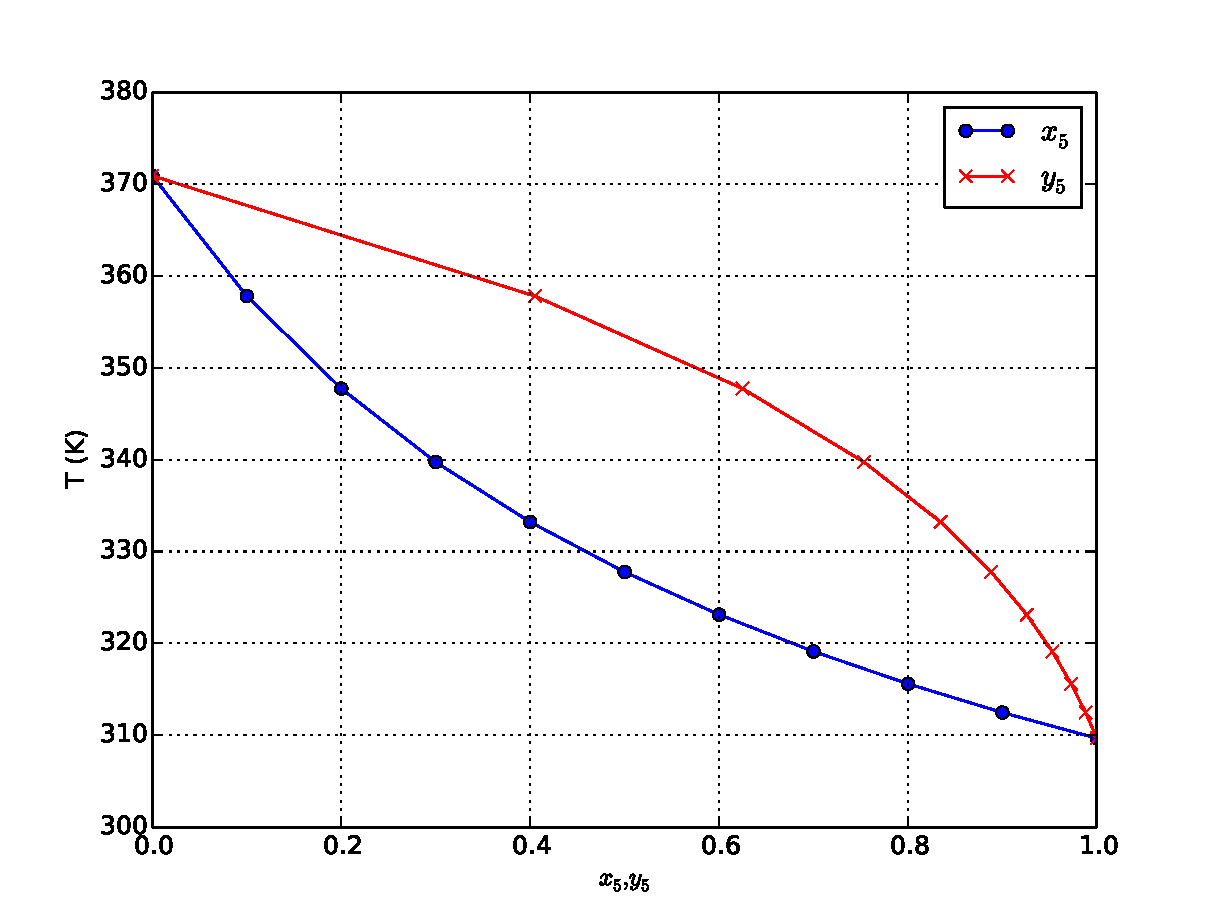
\includegraphics[width=.5\linewidth,clip]{./Figs/Mod4Ex2b}}}
         \caption{Example~\ref{Mod04Ex02}}
      \end{figure}
\clearpage
 % 
%%%
%%% EXAMPLE
%%%
   \item\label{Mod04Ex03} Estimate the bubble and dew point temperatures of a mixture of 25 mol-$\%$ of n-pentane, 45 mol-$\%$ of n-hexane and 30 mol-$\%$ of n-heptane at 1.013 bar. Given $P^{\text{sat}}$ relation,
    \begin{displaymath}
      \ln{P_{i}^{\text{sat}}} = A_{i} - \frc{B_{i}}{RT}
    \end{displaymath}
    with $A_{nC_{5}}=10.422$, $A_{nC_{6}}=10.456$, $A_{nC_{7}}=11.431$, $B_{nC_{5}}=26799 \text{ J.mol}^{-1}$, $B_{nC_{6}}=29676 \text{ J.mol}^{-1}$ and $B_{nC_{7}}=35200 \text{ J.mol}^{-1}$. Also [$P$] = bar and [$T$] = K.

% SOLUTION
 \noindent{\bf Solution:} Assuming the solution is ideal and the gas phase behaves as an ideal gas (\ie low/room pressure), Raoult's law can be used,
    \begin{displaymath}
       x_{i}P_{i}^{\text{sat}} = y_{i}P = P_{i} \;\;\text{ with }\;\; \summation[x_{i}P_{i}^{\text{sat}}]{i}{} = \summation[P_{i}]{i}{} = P, \;\summation[x_{i}]{i}{}=1=\summation[y_{i}]{i}{}.
    \end{displaymath}
    For the bubble point, the procedure is:
    \begin{enumerate}[i)]
       \item choose an initial guess for the bubble point temperature, $T^{\text{guess}}$;
       \item calculate $y_{i}=\frc{x_{i}P_{i}^{\text{sat}}}{P}$;
       \item then:
           \begin{itemize}
              \item if $\summation[y_{i}]{i}{} = 1 \;\;\Rightarrow \;\; T^{\text{guess}} = T$;
              \item if $\summation[y_{i}]{i}{} > 1 \;\;\Rightarrow \;\; T^{\text{guess}} > T \;\; \Rightarrow\;\; \text{adjust } T^{\text{guess}}$;
              \item if $\summation[y_{i}]{i}{} < 1 \;\;\Rightarrow \;\; T^{\text{guess}} < T \;\; \Rightarrow\;\; \text{adjust } T^{\text{guess}}$.
           \end{itemize}
    \end{enumerate}
    Thus, for this problem,
    \begin{displaymath}
        \summation[y_{i}]{i}{} = 1\;\; \Longleftrightarrow \;\; \frc{x_{5}P_{5}^{\text{sat}}}{P} + \frc{x_{6}P_{6}^{\text{sat}}}{P} + \frc{x_{7}P_{7}^{\text{sat}}}{P} = 1,
    \end{displaymath}
    where $P_{i}^{\text{sat}}$ is a function of $T$, 
    \begin{displaymath}
        \frc{x_{5}\exp{\left(A_{5}-\frc{B_{5}}{RT}\right)}}{P} + \frc{x_{6}\exp{\left(A_{6}-\frc{B_{6}}{RT}\right)}}{P} + \frc{x_{7}\exp{\left(A_{7}-\frc{B_{7}}{RT}\right)}}{P} = 1
    \end{displaymath}
    Using $T^{\text{guess}}=298.15$ K as initial guess, $T=334.9380$ K (bubble point temperature). Now, calculating the vapour composition, $y_{i}=\frc{x_{i}P_{i}^{\text{sat}}}{P}$ leads to,
    \begin{displaymath}
        y_{5} =0.5483,\;\; y_{6} = 0.3634\;\;\text{ and }\;\;y_{7} = 0.0883\;\;\Rightarrow\;\; \summation[y_{i}]{i}{} = 1.0000
    \end{displaymath}

\medskip
    For the dew point, the procedure is:
    \begin{enumerate}[i)]
       \item choose an initial guess for the dew point temperature, $T^{\text{guess}}$;
       \item calculate $x_{i}=\frc{y_{i}P}{P_{i}^{\text{sat}}}$;
       \item then:
           \begin{itemize}
              \item if $\summation[x_{i}]{i}{} = 1 \;\;\Rightarrow \;\; T^{\text{guess}} = T$;
              \item if $\summation[x_{i}]{i}{} > 1 \;\;\Rightarrow \;\; T^{\text{guess}} < T \;\; \Rightarrow\;\; \text{adjust } T^{\text{guess}}$;
              \item if $\summation[x_{i}]{i}{} < 1 \;\;\Rightarrow \;\; T^{\text{guess}} > T \;\; \Rightarrow\;\; \text{adjust } T^{\text{guess}}$.
           \end{itemize}
    \end{enumerate}
    Thus, for this problem,
    \begin{displaymath}
        \summation[x_{i}]{i}{} = 1\;\; \Longleftrightarrow \;\; \frc{y_{5}P}{P_{5}^{\text{sat}}} + \frc{y_{6}P}{P_{6}^{\text{sat}}} + \frc{y_{7}P}{P_{7}^{\text{sat}}} = 1,
    \end{displaymath}
    where $P_{i}^{\text{sat}}$ is a function of $T$, 
    \begin{displaymath}
        \frc{y_{5}P}{\exp{\left(A_{5}-\frc{B_{5}}{RT}\right)}} + \frc{x_{6}P}{\exp{\left(A_{6}-\frc{B_{6}}{RT}\right)}} + \frc{x_{7}P}{\exp{\left(A_{7}-\frc{B_{7}}{RT}\right)}}= 1
    \end{displaymath}
    Using $T^{\text{guess}}=298.15$ K as initial guess, $T=350.5857$ K (dew point temperature). Now, calculating the liquid composition, $y_{i}=\frc{x_{i}P_{i}^{\text{sat}}}{P}$ leads to,
    \begin{displaymath}
        x_{5} =0.0742\;\; x_{6} = 0.3463\;\;\text{ and }\;\;x_{7} = 0.5795\;\;\Rightarrow\;\; \summation[x_{i}]{i}{} = 1.0000
    \end{displaymath}


\clearpage
 % 
 % 
%%%
%%% EXAMPLE
%%%
   \item\label{Mod04Ex04} Estimate the bubble and dew point pressures of a mixture of 25 mol-$\%$ of n-pentane, 45 mol-$\%$ of n-hexane and 30 mol-$\%$ of n-heptane at 73$^{\circ}$C. Given $P^{\text{sat}}$ relation,
    \begin{displaymath}
      \ln{P_{i}^{\text{sat}}} = A_{i} - \frc{B_{i}}{RT}
    \end{displaymath}
    with $A_{nC_{5}}=10.422$, $A_{nC_{6}}=10.456$, $A_{nC_{7}}=11.431$, $B_{nC_{5}}=26799 \text{ J.mol}^{-1}$, $B_{nC_{6}}=29676 \text{ J.mol}^{-1}$ and $B_{nC_{7}}=35200 \text{ J.mol}^{-1}$. Also [$P$] = bar and [$T$] = K.

% SOLUTION
 \noindent{\bf Solution:}  For the bubble point, the mixture follows Raoult's law at 73$^{\circ}$C,
      \begin{displaymath}
          P = \summation[x_{i}P_{i}^{\text{sat}}]{i}{} = x_{5}P_{5}^{\text{sat}} + x_{6}P_{6}^{\text{sat}} + x_{7}P_{7}^{\text{sat}} = 1.413\text{ bar}
      \end{displaymath}
      This is the bubble point pressure at 346.15 K. The composition of the vapour phase is,
      \begin{displaymath}
             y_{i}=\frc{x_{i}P_{i}^{\text{sat}}}{P}
             \begin{cases}
                  y_{5} = 0.5370,\\
                  y_{6} = 0.3680,\\
                  y_{7} = 0.0950,
             \end{cases}
      \end{displaymath}
      leading to $\summation[y_{i}]{i}{} = 1.0000$.

\medskip

     For the dew point, the procedure is:
    \begin{enumerate}[i)]
       \item choose an initial guess for the dew point pressure, $P^{\text{guess}}$;
       \item calculate $x_{i}=\frc{Py_{i}}{P_{i}^{\text{sat}}}$;
       \item then:
           \begin{itemize}
              \item if $\summation[x_{i}]{i}{} = 1 \;\;\Rightarrow \;\; P^{\text{guess}} = P$;
              \item if $\summation[x_{i}]{i}{} > 1 \;\;\Rightarrow \;\; P^{\text{guess}} > P \;\; \Rightarrow\;\; \text{adjust } P^{\text{guess}}$;
              \item if $\summation[x_{i}]{i}{} < 1 \;\;\Rightarrow \;\; P^{\text{guess}} < P \;\; \Rightarrow\;\; \text{adjust } P^{\text{guess}}$.
           \end{itemize}
    \end{enumerate}
    Thus, for this problem,
    \begin{displaymath}
        \summation[x_{i}]{i}{} = 1\;\; \Longleftrightarrow \;\; \frc{y_{5}P}{P_{5}^{\text{sat}}} + \frc{y_{6}P}{P_{6}^{\text{sat}}} + \frc{y_{7}P}{P_{7}^{\text{sat}}} = 1,
    \end{displaymath}
    where $P_{i}^{\text{sat}}$ is a function of $T$ (which is known in this problem!).  Solving this equation leads to $P=0.8774$ bar (dew point pressure) with composition
    \begin{displaymath}
        x_{5} =0.0723\;\; x_{6} = 0.3418\;\;\text{ and }\;\;x_{7} = 0.5859\;\;\Rightarrow\;\; \summation[x_{i}]{i}{} = 1.0000
    \end{displaymath}


\clearpage
 % 
 % 
%%%
%%% EXAMPLE
%%%
   \item\label{Mod04Ex045} A liquid mixture of 25 mol-$\%$ n-pentane $\left(nC_{5}\right)$, 45 mol-$\%$ n-hexane $\left(nC_{6}\right)$ and 30 mol-$\%$ n-heptane $\left(nC_{7}\right)$ initially at 69$^{\circ}$C and a high pressure, is partially vaporised by isothermically lowering the pressure to  1.013 bar. Calculate the relative amounts of vapour and liquid in equilibrium and compositions.

% SOLUTION
 \noindent{\bf Solution:} This is a typical {\it flash} problem described by the figure,
    
  \begin{figure}[h]
     \begin{center}
         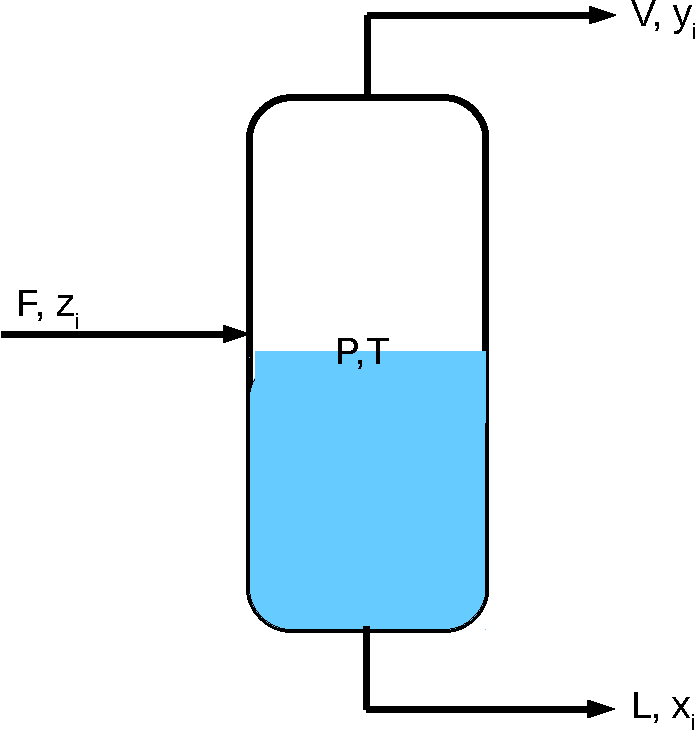
\includegraphics[width=.25\linewidth,clip]{./Figs/FlashDistillation}
     \end{center}
     \caption{Schematic of a flash distillation process, Example~\ref{Mod04Ex045}.}
  \end{figure}

From the given $P_{i}^{\text{sat}}$ relation at 69$^{\circ}$C,
   \begin{displaymath}
        \begin{cases}
            P_{5}^{\text{sat}} = 2.721 \text{ bar},\\ 
            P_{6}^{\text{sat}} = 1.024 \text{ bar},\\
            P_{7}^{\text{sat}} = 0.389 \text{ bar}.
        \end{cases}
   \end{displaymath}
Assuming ideal solution, $K_{i}$ for the three hydrocarbons can be readily obtained,
   \begin{displaymath}
        K_{i} = \frc{P_{i}^{\text{sat}}}{P} = \frc{y_{i}}{x_{i}},
          \begin{cases}
             K_{5} = 2.6861; \\
             K_{6} = 1.0109; \\
             K_{7} = 0.3840
          \end{cases}
   \end{displaymath}
   Therefore,
   \begin{displaymath}
       y_{5} = x_{5}K_{5},\;\;\;y_{6} = x_{6}K_{6},\;\;\;y_{7} = x_{7}K_{7},
   \end{displaymath}
    with the molar fraction constraints,
    \begin{displaymath}
        \begin{cases}
            x_{5}+x_{6}+x_{7} = 1,\\ 
            y_{5}+y_{6}+y_{7} = 1, \\
            F = V + L
        \end{cases}
   \end{displaymath}
   Assuming $F=1$, the mass balance of the individual components in equilibrium are
    \begin{displaymath}
        \begin{cases}
            x_{5}L + y_{5}V = z_{5} = 0.25 \\
            x_{6}L + y_{6}V = z_{6} = 0.45 \\
            x_{7}L + y_{7}V = z_{7} = 0.30            
        \end{cases}
   \end{displaymath}
   these relation can be rewritten as $\left(\text{based on }y_{5}+y_{6}+y_{7} = 1,\; y_{i}=K_{i}x_{i} \;\text{ and } V= 1-L\right)$
    \begin{displaymath}
        \begin{cases}
            x_{5}L + y_{5}V = z_{5} = 0.25 \;\Longrightarrow\; x_{5}\left[L\left(1-K_{5}\right)+K_{5}\right] = 0.25 \\
            x_{6}L + y_{6}V = z_{6} = 0.45 \;\Longrightarrow\; x_{6}\left[L\left(1-K_{6}\right)+K_{6}\right] = 0.45 \\
            x_{7}L + y_{7}V = z_{7} = 0.30 \;\Longrightarrow\; x_{7}\left[L\left(1-K_{7}\right)+K_{7}\right] = 0.30
        \end{cases}
   \end{displaymath}


   Now the molar fraction constraint of the liquid phase $x_{5}+x_{6}+x_{7} = 1$, is
   \begin{displaymath}
        \frc{0.25}{L\left(1-K_{5}\right)+K_{5}} + \frc{0.45}{L\left(1-K_{6}\right)+K_{6}} + \frc{0.30}{L\left(1-K_{7}\right)+K_{7}} = 1
   \end{displaymath}
   This expression has just one unknown, $L$, as a cubic polynomial. Solving with initial guess $L^{\text{guess}}=0.50$ leads to $L=0.5748$.  Now using 
    \begin{displaymath}
        \begin{cases}
            x_{5}L + y_{5}V = z_{5} = 0.25 \;\Longrightarrow\; x_{5}\left[L\left(1-K_{5}\right)+K_{5}\right] = 0.25  \;\Longrightarrow\;  x_{5} = 0.1456 \\
            x_{6}L + y_{6}V = z_{6} = 0.45 \;\Longrightarrow\; x_{6}\left[L\left(1-K_{6}\right)+K_{6}\right] = 0.45  \;\Longrightarrow\;  x_{6} = 0.4479 \\
            x_{7}L + y_{7}V = z_{7} = 0.30 \;\Longrightarrow\; x_{7}\left[L\left(1-K_{7}\right)+K_{7}\right] = 0.30  \;\Longrightarrow\;  x_{7} = 0.4065 
        \end{cases}
   \end{displaymath}
   leading to $\summation[x_{i}]{i}{} = 1.0000$. Molar fraction of the vapour phase is $V= 1-L=0.4252$, resulting in
    \begin{displaymath}
        \begin{cases}
            y_{5} = K_{5}x_{5} \;\Longrightarrow\; y_{5} = 0.3911 \\
            y_{6} = K_{6}x_{6} \;\Longrightarrow\; y_{6} = 0.4528 \\
            y_{7} = K_{7}x_{7} \;\Longrightarrow\; y_{7} = 0.1561 
        \end{cases}
   \end{displaymath}
    with $\summation[y_{i}]{i}{} = 1.0000$
 % 

%
\end{enumerate}

\clearpage
%%%%%%%%%%%%%%%%%%%%%%%%%%%%%%%%%%%%%%%%%%%%%%%%%%%%%%%%%%%%%%%%%%%%%%%%%%%%%%%%%%%%%%%%%%%%%%%%%%%%%%%%%%%%%%%%%%%%%%%%%%%%%%%%%%%%%%%%%%%%%%
%%%%%%%%%%%%%                                                    END OF MODULE 04                                                %%%%%%%%%%%%%
%%%%%%%%%%%%%%%%%%%%%%%%%%%%%%%%%%%%%%%%%%%%%%%%%%%%%%%%%%%%%%%%%%%%%%%%%%%%%%%%%%%%%%%%%%%%%%%%%%%%%%%%%%%%%%%%%%%%%%%%%%%%%%%%%%%%%%%%%%%%%%

%%%
%%% SECTION
%%%
\section{Module 05: Solution Thermodynamics}\label{Section:05}

%%% SUBSUBSECTION
\subsection{Introduction}\label{Section:05:Introduction}
Vapour-liquid equilibrium of pure components and mixtures were the focus of study in Modules~\ref{Section:02}-\ref{Section:04}. In this modules, equations of state were introduced to represent the $PVT$ behaviour of pure components in both vapour and liquid phases. From your readings, you may have noticed that EOS are largely applied, with relatively accuracy, to vapour phases, but rarely used to assess liquid phase behaviour. 

This is mainly due to the fact that EOS were originally (and cubic EOS in particular) to represent weak inter-molecular forces between gaseous molecules at relatively large distances (\ie {\it mean free path}). As pressure increases $\left(P\rightarrow \infty\right)$ and the distance between molecules tends to zero $\left(d\rightarrow 0\right)$, the accuracy of equations of state to predict $PVT$ behaviour also decreases, as the attractive and repulsive forces between molecules become stronger. 

Molecules in liquid phase are held together at close distances by strong attractive forces, however these forces are not strong enough to keep them in fixed positions (as inter-/intra-molecular forces in the solid phase) and the molecules are free to move past, slide over and collide with other molecules. A fraction of the molecules (mostly with higher energy) may be able to break such attractive forces and `escape' towards the vapour phase. 

Kinetic energy in gaseous molecules are larger than the attractive forces, leading to large distances between molecules and a tendency to occupy the whole volume of the system. The large kinetic energy in gaseous molecules also lead to continuous collisions between molecules and with the system (container) walls. During collisions, although total momentum is conserved, individual energies (and velocities) may decrease and molecules may move to a system with lower kinetic energy, \ie liquid phase.

\bigskip

In Module~\ref{Section:01}, the concept of {\it mechanical} (\ie system at constant or uniform pressure) and {\it thermal} (from the Zeroth law) equilibrium were introduced. In order to define phase equilibria, we established (in Module~\ref{Section:04}) that an additional condition was necessary, {\it chemical equilibrium}, \ie equality of Gibbs free energy of all phases (Section~\ref{Section:03:ClapeyronRelations}) for pure fluids. This concept can be extended for mixtures by using the definition of {\it chemical potential}, $\mu_{i}$ (Eqn.~\ref{Mod04_ChemPotentialDef1b}),
         \begin{displaymath}
            \mu_{i} = \Partial[(nG)]{n_{i}}{T,P,n_{j\ne i}} \;\;\Longleftrightarrow\;\; \mu_{i} = \overline{G}_{i},
         \end{displaymath}
where $\overline{G}_{i}$ is the {\it partial molar Gibbs free energy}. This leads to the final phase equilibria condition in which {\it the chemical potential for each component at all coexisting phases are identical}, \ie 
         \begin{eqnarray}
            && \mfr[\mu]{i}{\alpha} = \mfr[\mu]{i}{\beta} = \cdots =  \mfr[\mu]{i}{j} = \cdots = \mfr[\mu]{i}{\mathcal{N}_{\mathcal{P}}} = \;\;\;\forall i\in\{1,2,\cdots,\mathcal{C}\}\;\; \text{ and }\;\;\; \forall j\in\{\alpha,\beta,\cdots,\mathcal{N}_{\mathcal{P}}\}, \nonumber \\
            &&  \text{or for VLE systems: }\;\;\;\; \mfr[\mu]{i}{L} = \mfr[\mu]{i}{V},\;\;\;\forall i\in\{1,2,\cdots,\mathcal{C}\} \nonumber 
         \end{eqnarray}

\medskip

The main assumptions for ideal gas behaviour assume that molecules of gas are massless particles with no interaction between them (\ie volume of the molecules is negligibly small compared with the volume occupied by the gas or simply the distance between gaseous molecules are often infinitely large, $d\rightarrow \infty$), except during elastic collisions over negligible duration. These conditions can only be met by fluids at sufficiently high temperature and relatively low pressure when large distances between molecules and high velocity overcome any interaction. The concept of ideality for liquids also exists and is based on the assumption that inter-molecular forces are the same between all molecules in solution. This assumption may be correct for pure non-polar substances (\ie in solutions with no major inter-/intra-molecular forces).

Thus, the aim of this Module is to define thermodynamic properties of real solutions based on properties of ideal solutions. Excess properties (Section~\ref{Section:04:ExcessProperties}) plays a role similar to that of residual properties (Section~\ref{Section:03:ResidualProperties}) for gases. In order to study solution properties at low to moderate pressures, {\it activity coefficient}, based on the definition of {\it fugacity}, is used. The {\it activity coefficient}, derived from the {\it excess Gibbs free energy}, is a measure of the extent of non-ideality of a real solution and helps describing phase equilibria of mixtures at low and moderate pressures.


%%% SUBSECTION
\subsection{Fugacity}\label{Section:05:FugacitySection}
\begin{subequations}
  A formal definition for {\it partial molar property} was introduced in Section~\ref{Section:04:PartialMolarProperties} for an arbitrary extensive function $M$, Eqn.~\ref{Mod04_PartialProperties2}. Such formulation was applied to the Gibbs free energy of a system with $n=n_{1}+n_{2}+\cdots+n_{\mathcal{C}}$ moles leading to the definition of the {\it chemical potential}, Eqns.~\ref{Mod04_ChemPotentialDef1}-~\ref{Mod04_ChemPotentialDef1b},
  \begin{shaded}
     \begin{eqnarray}
       && dG = \Partial[G]{P}{T,n}dP + \Partial[G]{T}{P,n}dT + \underbrace{\Partial[G]{n}{T,P}}_{\mu}dn, \nonumber \\
       && \mu_{i} = \Partial[(nG)]{n_{i}}{T,P,n_{j\ne i}} \;\;\Longleftrightarrow\;\; \mu_{i} = \overline{G}_{i}, \nonumber
     \end{eqnarray}
  \end{shaded}
  \noindent For pure components,
  \begin{displaymath}
    G = n\mu \;\;\rightarrow \mu=\frc{G}{n}=\overline{g},
  \end{displaymath}
  where $\overline{g}$ is the molar Gibbs free energy. Using the Maxwell relation, Eqn.~\ref{Mod03_MaxwellRelation7},
  \begin{eqnarray}
    && \Partial[G]{P}{T} = V = \Partial[n\mu]{P}{T} = n\Partial[\mu]{P}{T} \nonumber \\
    && \Partial[\mu]{P}{T} = \frc{V}{n} = \overline{v}\label{Mod05_fugacity1}
  \end{eqnarray}
  where $\underline{v}$ is the molar volume. For an ideal gas,
  \begin{displaymath}
     \Partial[\mu^{\text{ig}}]{P}{T} = \frc{RT}{P},
  \end{displaymath}
  where the superscript $^{\text{ig}}$ refers to ideal gas. This differential can be integrated as,
  \begin{equation}
    \mu^{\text{ig}} = RT\ln{P} + C(T),\label{Mod05_fugacity1a}
  \end{equation}
  where $C(T)$ is an integration constant. At limiting conditions, $P\rightarrow 0$ and $P\rightarrow\infty$, the chemical potential lies within $-\infty < \mu < +\infty$. For a fluid to be considered an ideal gas, pressure needs to be relatively low, thus we can use Eqn.~\ref{Mod05_fugacity1a} to represent the chemical potential of real fluids,
  \begin{equation}
    \mu = RT\ln{f} + C(T),\label{Mod05_fugacity1b}
  \end{equation}
  where $f$ is the {\it fugacity of a real gas}, \ie \blue{a representation of the pressure of an ideal gas that has the same chemical potential as the real gas.} Since the {\it fugacity} has the \underline{units of pressure}, it is often referred as a `fictitious pressure'.  The definition of fugacity from Eqn.~\ref{Mod05_fugacity1b} is entirely general and can be readily extended to both liquids and solids. Now, replacing Eqn.~\ref{Mod05_fugacity1b} in the Maxwell relation, Eqn.~\ref{Mod03_MaxwellRelation7}, at constant temperature,
  \begin{equation}
    RT\Partial[\left(\ln{f}\right)]{P}{T} = \overline{v}.\label{Mod05_fugacity1c}
  \end{equation}
  {\it Fugacity} can be obtained by integrating this equation holding $T$ constant. As pressure tends to zero (lower limit of the left-hand-side integration), the fluid behaves as an ideal gas. We can thus state that the fugacity of a pure component is equal to the pressure in the limit of zero pressure, \ie
      \begin{shaded}
        \begin{equation}
           \lim\limits_{P \rightarrow 0} \frc{f}{P} = 1.\label{Mod05_fugacity1d}
        \end{equation}
      \end{shaded}

  \noindent  In a \underline{mixture} containing $n$ moles of $\mathcal{C}$ chemical species, Eqn.~\ref{Mod05_fugacity1c} becomes,
      \begin{eqnarray}
        && RT\Partial[\left(\ln{f_{i}}\right)]{P}{T,n} = \overline{v}_{i},\;\;\;\;\forall i\in\left\{1,2,\cdots,\mathcal{C}\right\}\label{Mod05_fugacity1e1} \\
        && RT\Partial[\left(\ln{\overline{f}_{i}}\right)]{P}{T,n} = \overline{V}_{i},\label{Mod05_fugacity1e2}
      \end{eqnarray}
      where $f_{i}$ is the {\it fugacity of pure component $i$} and $\overline{f}_{i}$ is the {\it fugacity of component $i$ in the mixture}. $\overline{v}_{i}$ and $\overline{V}_{i}$ are the molar volume of pure component $i$ and, of component $i$ in the mixture. If we subtract Eqn.~\ref{Mod05_fugacity1e1} from ~\ref{Mod05_fugacity1e2} and integrate the result from $P'$ to $P$ at constant $T$,
      \begin{displaymath}
        RT\Partial[\left(\ln{\frc{\overline{f}_{i}}{f_{i}}}\right)]{P}{T,n} = \overline{V}_{i} - \overline{v}_{i} \;\;\Longrightarrow \;\;  RT\left[\left.\ln{\left(\frc{\overline{f}_{i}}{f_{i}}\right)}\right|_{P'}^{P}\right] = \int\limits_{P'}^{P}\left(\overline{V}_{i} - \overline{v}_{i}\right)dP
      \end{displaymath}
      Assuming that $P'$ tends to $0$,
      \begin{equation}
        RT\left[\ln{\left(\frc{\overline{f}_{i}}{f_{i}}\right)} - \lim\limits_{P'\rightarrow 0}\ln\left(\frc{\overline{f}_{i}}{f_{i}}\right)\right] = \int\limits_{0}^{P}\left(\overline{V}_{i} - \overline{v}_{i}\right)dP.\label{Mod05_fugacity1f}
      \end{equation}
      When $P'\rightarrow 0$
      \begin{displaymath}
        \begin{cases}
          f_{i} \rightarrow P', \\
          \overline{f}_{i} \rightarrow y_{i}P',
        \end{cases}
      \end{displaymath}
      and the limiting term in the previous equation becomes,
      \begin{displaymath}
        \lim\limits_{P'\rightarrow 0}\ln\left(\frc{\overline{f}_{i}}{f_{i}}\right) \rightarrow \ln{\left(\frc{y_{i}P'}{P'}\right)} = \ln{y_{i}}
      \end{displaymath}
      Thus Eqn.~\ref{Mod05_fugacity1f} becomes,
        \begin{displaymath}
          RT\left[\ln{\left(\frc{\overline{f}_{i}}{f_{i}}\right)} - \ln{y_{i}}\right] = \int\limits_{0}^{P}\left(\overline{V}_{i} - \overline{v}_{i}\right)dP
        \end{displaymath}
      \begin{shaded}
        \begin{equation}
           RT\ln{\left(\frc{\overline{f}_{i}}{y_{i}f_{i}}\right)} = \int\limits_{0}^{P}\left(\overline{V}_{i} - \overline{v}_{i}\right)dP. \label{Mod05_fugacity1g}
        \end{equation}
      \end{shaded}
  \noindent This expression relates fugacity of a pure component $i$ and the fugacity of the same component $i$ in a mixture with $\mathcal{C}$ chemical components during continuous change in pressure. The term in brackets in the left-hand side represents in the ratio between partial pressures between real and ideal fluids in a mixture.

        
      For an ideal mixture of ideal gases, the partial pressure of species $i$ is the fugacity of component $i$ in the mixture, \ie
         \begin{displaymath}
            \mfr[\overline{f}]{i}{V} = y_{i}P = P_{i}.
         \end{displaymath}
      Now, for an ideal mixture of real fluids,
         \begin{displaymath}
            \mfr[\overline{f}]{i}{L} = x_{i}\mfr[f]{i}{L},
         \end{displaymath}
      \ie the fugacity of a component in a mixture is a function of the fugacity of the pure component.
      \begin{shaded}
         An \underline{ideal solution} is a mixture in which,
        \begin{equation}
          \mfr[\overline{f}]{i}{V} = y_{i}P = P_{i}\;\;\;\text{ and }\;\;\; \mfr[\overline{f}]{i}{L} = x_{i}\mfr[f]{i}{L}\label{Mod05_fugacity2a}
        \end{equation}
        These expressions are called \red{\it Lewis-Randall rules} and they describe relations between phase compositions and fugacities.
      \end{shaded}
      
\end{subequations}

      
%%% SUBSECTION
\subsection{Activity and Activity Coefficient }\label{Section:05:ActivitySection}
   \begin{subequations}
        
      In a mixture (based on Eqn.~\ref{Mod05_fugacity1b}),
        \begin{displaymath}
           \mu_{i} = RT\ln{\overline{f}_{i}} + C_{i}(T),
        \end{displaymath}
      consider a reference-state, where a species $i$ of a multi-component system is pure at temperature $T$ and at reference-state pressure, $P_{\text{ref}}$,
        \begin{equation}
           \mu_{i} - \mu_{i}^{\circ} = RT\ln{\left(\frc{\overline{f}_{i}}{f_{i}^{\circ}}\right)},\label{Mod05_activity1a}
        \end{equation}
      where superscript $^{\circ}$ stands for {\it reference state}. 
        \begin{shaded}
           \noindent Now, we can define the term in brackets as the \blue{activity} (dimensionless)
           \begin{equation}
              \frc{\overline{f}_{i}}{f_{i}^{\circ}} = a_{i}, \label{Mod05_activity1b}
           \end{equation}
           which `measures' the deviation from ideal behaviour.
        \end{shaded}
      \noindent Since $\mu^{\circ} = \overline{g}^{\circ}_{i}$, Eqn.~\ref{Mod05_activity1a} becomes
        \begin{equation}
           \mu_{i} = \overline{g}^{\circ}_{i} + RT\ln{a_{i}}\label{Mod05_activity1c}
        \end{equation}
      For an ideal solution, the {\it Lewis-Randall relation} can be used,
        \begin{displaymath}
           a_{i} =  \frc{\overline{f}_{i}}{f_{i}^{\circ}} = \frc{y_{i}f_{i}}{f_{i}^{\circ}},
        \end{displaymath}
      where $f_{i}$ is the fugacity of pure component $i$ at $P$ and $T$, and $f_{i}^{\circ}$ is the fugacity of pure component $i$ at $T$ and the reference-pressure $P_{\text{ref}}$. Thus,
        \begin{displaymath}
           \mu_{i} = \overline{g}^{\circ}_{i} + RT\ln{\left( \frc{y_{i}f_{i}}{f_{i}^{\circ}}\right)}.
        \end{displaymath}

        \begin{shaded}
            \noindent For \underline{\it ideal solutions},
              \begin{equation}
                 \mu_{i} = \overline{g}^{\circ}_{i} + RT\ln{\left[\left(\frc{f_{i}}{P}\right)\left(\frc{P_{\text{ref}}}{f_{i}^{\circ}}\right)\frc{y_{i}P}{P_{\text{ref}}}\right]}.\label{Mod05_activity1d}
              \end{equation}
            If component $i$ behaves as an \underline{\it ideal gas} at both $\left(T,P\right)$ and $\left(T,P_{\text{ref}}\right)$, thus $\frc{f_{i}}{P} = \frc{f_{i}^{\circ}}{P_{\text{ref}}}=1$ and Eqn.~\ref{Mod05_activity1d} becomes
              \begin{equation}
                 \mu_{i} = \overline{g}^{\circ}_{i} + RT\ln{\frc{y_{i}P}{P_{\text{ref}}}}.\label{Mod05_activity1e}
              \end{equation}
             This expression allows the calculation of the chemical potential of the vapour phase in a mixture subjected to a change in pressure based on composition and temperature. Molar Gibbs energy at reference conditions, $\overline{g}^{\circ}_{i}$, for several chemical species are often tabulated and can be found in any chemical engineering handbook.
\medskip
             
        \noindent Finally, we can now define the \underline{\blue{activity coefficient}}, $\gamma_{i}$, as
          \begin{equation}
              a_{i} = \frc{y_{i}f_{i}}{f_{i}^{\circ}}\;\;\;\;\Rightarrow \;\;\;\; \gamma_{i} = \frc{a_{i}}{y_{i}} = \frc{f_{i}}{f_{i}^{\circ}}\label{Mod05_activity1f}
          \end{equation}
         And for solutions,
          \begin{equation}
              \gamma_{i} = \frc{\overline{f}_{i}}{x_{i}f_{i}}\label{Mod05_activity1g}
          \end{equation}
         The \underline{\blue{activity coefficient}} takes into account non-idealities in the liquid phase, and it first appeared in the slide (handouts) of Module~\ref{Section:04} on VLE of non-ideal mixtures. Now, we can properly define the \underline{Raoult's law} (Section~\ref{Section:04:RaoultsLaw}) at low pressure,
          \begin{equation}
               \gamma_{i} = \frc{\overline{f}_{i}}{x_{i}f_{i}} = \frc{y_{i}P}{x_{i}f_{i}}=\frc{y_{i}P}{x_{i}P_{i}^{\text{sat}}} \;\;\;\Longrightarrow \;\;\;\ x_{i}\gamma_{i}P_{i}^{\text{sat}} = y_{i}P \label{Mod05_RaoultLaw}
          \end{equation}
          Equation~\ref{Mod05_RaoultLaw} is the general form for Raoult's law. If the solution is ideal, $\gamma_{i}=1$ and Eqn.~\ref{Mod04_RaoultLaw} is recovered.

      \end{shaded}       
%
   \end{subequations}
      
%%% SUBSECTION
\subsection{Henry's Law}\label{Section:05:HenryLaw}
 %
Now that the concepts of fugacity and activity coefficient were introduced, we can return to the special VLE condition in which the solute is very diluted in the mixture (Section~\ref{Section:04:HenryLaw}). In such cases, the fugacity of a very dilute chemical species in a liquid mixture (\eg dissolved gases or solid of limited solubility) is experimentally found to be a linear function of its low composition (\ie mole fraction)\footnote{It is clear that the division in the limiting term,
  \begin{displaymath}
    \lim\limits_{x_{i}\rightarrow 0}\frc{\overline{f_{i}}}{x_{i}}
  \end{displaymath}
  is undetermined as when $x_{i}\rightarrow 0,\;\;f_{i}=0$, \ie at infinite dilution of a solute $i$ in solution, the fugacity of this component is null. In order to solve this mathematical problem, we can use the L'H\^opital rule (see Appendix D4) which states that for a limit,
         \begin{displaymath}
                 \lim\limits_{x\rightarrow a}\frc{f(x)}{g(x)},
         \end{displaymath}
         if the numerator and denominator are finite at $a$, and $g(a)=0$, then
         \begin{displaymath}
                 \lim\limits_{x\rightarrow a}\frc{f(x)}{g(x)} =  \lim\limits_{x\rightarrow a}\frc{f'(a)}{g'(a)}.
         \end{displaymath}
         Therefore, the limiting dilution case can be solved as
         \begin{displaymath}
                 \lim\limits_{x_{i}\rightarrow 0}\frc{\overline{f_{i}}}{x_{i}} = \left(\frc{d \overline{f_{i}}}{d x_{i}}\right)_{x_{i}=0},
         \end{displaymath}
}, \ie   
      \begin{eqnarray}
        && \lim\limits_{x_{i}\rightarrow 0}\frc{\overline{f_{i}}}{x_{i}} = \left(\frc{d \overline{f_{i}}}{d x_{i}}\right)_{x_{i}=0}  \equiv \mathcal{H}_{i}, \nonumber \\
        && \mfr[\overline{f}]{i}{L}(T,P,x) = x_{i}\mathcal{H}_{i}(T,P)\;\;\;\;\text{ as } x_{i}\rightarrow 0.
      \end{eqnarray}      
This proportionality constant, $\mathcal{H}$, is called \blue{\it Henry's law constant}, and is dependent on the solute-solvent pair, temperature and pressure. This experimentally-defined constant was first introduced in Eqn.~\ref{Mod04_HenryLaw} as, in equilibrium conditions (at $P$, $T$ and $n$ constants), $\mfr[\overline{f}]{i}{V}=\mfr[\overline{f}]{i}{L}$,
         \begin{shaded}
           \begin{displaymath}
             P_{i} = y_{i}P = x_{i}\mathcal{H}_{i},
           \end{displaymath}
           with $\mfr[\overline{f}]{i}{V}=y_{i}P$.
        \end{shaded}
%

      
%%% SUBSECTION
\subsection{Gibbs-Duhem Equation}\label{Section:05:GibbsDuhem}
   \begin{subequations}
%
       In Section~\ref{Section:04:PartialMolarProperties}, the concept of \underline{\it partial molar property} of species $i$ in solution was defined as
         \begin{displaymath}
            \overline{M}_{i} = \Partial[(nM)]{n_{i}}{T,P,n_{j\ne i}},
         \end{displaymath}
        \ie the change of the total property $nM$ of a mixture of $\mathcal{C}$ species resulting from the addition at constant $T$ and $P$ of infinitesimal amount of species $i$ to a prescribed amount of solution.  It is important to bear in mind that \underline{\it partial molar property} of a substance is different from {\it molar property} of the same substance in a pure state at the same $T$ and $P$. This is due to inter-/intra-molecular forces that imposes interactions between species in solution.
\medskip

      Equation~\ref{Mod04_PartialProperties2} is a general expression for the change of any extensive property, $M$
         \begin{displaymath}
            d(nM) = n\Partial[M]{P}{T,x}dP + n\Partial[M]{T}{P,x}dT + \summation[\overline{M}_{i}dn_{i}]{i}{}.
         \end{displaymath}
      Mole fraction of a species $i$ was also introduced in Section~\ref{Section:04:Compositions} as,
         \begin{displaymath}
            x_{i} = \frc{n_{i}}{n} \;\;\Rightarrow\;\; n_{i} = x_{i}n,
         \end{displaymath}
      Applying {\it derivative of a product} rule on $n_{i}$,
         \begin{displaymath}
             dn_{i} = x_{i}dn + n dx_{i},
         \end{displaymath}
      and for the total property $(nM)$,
         \begin{displaymath}
             d(nM) = n d M + M dn.
         \end{displaymath}
      Replacing these expressions in Eqn.~\ref{Mod04_PartialProperties2},
        \begin{displaymath}
           n d M + M d n = n \Partial[M]{T}{P,x}dT + n\Partial[M]{P}{T,x}dP + \summation[\overline{M}_{i}\left(x_{i}dn + ndx_{i}\right)]{i}{}
        \end{displaymath}
      Rearranging this expression,
        \begin{equation}
           \underbrace{\left[dM - \Partial[M]{T}{P,x}dT - \Partial[M]{P}{T,x}dP - \summation[\overline{M}_{i}dx_{i}]{i}{}\right]}_{A}n + \underbrace{\left[M-\summation[\overline{M}_{i}x_{i}]{i}{}\right]}_{B}dn = 0\label{Mod5_GibbsDuhem1a}
        \end{equation}
      Equation~\ref{Mod5_GibbsDuhem1a} is valid for any arbitrary values of $n$ and $dn$, therefore $n$ and $dn$ should be independent of each other. Thus, this expression is only true if the coefficients $A$ and $B$ are zero, \ie
          \begin{eqnarray}
              A &=& dM - \Partial[M]{T}{P,x}dT - \Partial[M]{P}{T,x}dP - \summation[\overline{M}_{i}dx_{i}]{i}{} = 0 \nonumber \\
              dM &=& \Partial[M]{T}{P,x}dT + \Partial[M]{P}{T,x}dP + \summation[\overline{M}_{i}dx_{i}]{i}{}, \label{Mod5_GibbsDuhem1b}
          \end{eqnarray}
      and
          \begin{eqnarray}
              B &=& M-\summation[\overline{M}_{i}x_{i}]{i}{} = 0 \nonumber \\
              M &=& \summation[\overline{M}_{i}x_{i}]{i}{}\label{Mod5_GibbsDuhem1c} \\
             \text{as } nM = n\summation[\overline{M}_{i}x_{i}]{i}{} &\Rightarrow& dM = \summation[x_{i}d \overline{M}_{i}]{i}{} + \summation[\overline{M}_{i}dx_{i}]{i}{}\label{Mod5_GibbsDuhem1d}
          \end{eqnarray}
      Replacing Eqn.~\ref{Mod5_GibbsDuhem1d} in Eqn.~\ref{Mod5_GibbsDuhem1b} leads to the \blue{\it Gibbs-Duhem Equation (GDE)}
          \begin{shaded}
             \begin{equation}
                 \Partial[M]{T}{P,x}dT + \Partial[M]{P}{T,x}dP - \summation[x_{i}d\overline{M}_{i}]{i}{} = 0.\label{Mod5_GibbsDuhem1e}
             \end{equation}
             The \blue{GDE} must be satisfied for all changes in $P$, $T$ and $\overline{M}_{i}$.
          \medskip

             \noindent For changes at constant temperature and pressure conditions, the \blue{GDE} becomes
               \begin{equation}
                   \summation[x_{i}d\overline{M}_{i}]{i}{} = 0.\label{Mod5_GibbsDuhem1f}
               \end{equation}
             Or taking any arbitrary species $j$,
               \begin{equation}
                   \summation[x_{i}\frc{d\overline{M}_{i}}{dx_{j}}]{i}{} = 0, \;\;\;\text{ at constant } T\text{ and } P.\label{Mod5_GibbsDuhem1g}
               \end{equation}
             Equations~\ref{Mod5_GibbsDuhem1f}-\ref{Mod5_GibbsDuhem1g} imply that partial molar properties of various species, $\overline{M}_{i}$, are \underline{not} independent. Some key-properties,
               \begin{displaymath}
                   \begin{cases}
                       \lim\limits_{x_{i}\rightarrow 0}\overline{M}_{i} = \overline{M}_{i}^{\infty} & \text{\ie at infinite dilutions;} \\
                       \lim\limits_{x_{i}\rightarrow 1}\overline{M}_{i} = M_{i}                   & \text{ \ie nearly pure chemical species.} 
                   \end{cases}
               \end{displaymath}
          \end{shaded}
%
   \end{subequations}


      
%%% SUBSECTION
\subsection{Partial Molar Properties in Binary Solutions}\label{Section:05:PMP_Binary}
   \begin{subequations}
%
       In a mixture with $n$ moles, we can define the {\it isothermal molar property change of mixing}, $\Delta M_{\text{mix}}$ as,
          \begin{eqnarray}
              \Delta M_{\text{mix}}(T,P) & = & M(T,P) - \summation[x_{i}M_{i}(T,P)]{i}{} \nonumber \\
                                      &=& \underbrace{\summation[\overline{M}_{i}x_{i}]{i}{}}_{\text{from Eqn.~\ref{Mod5_GibbsDuhem1c}}} - \summation[x_{i}M_{i}]{i}{} \nonumber \\
                                      &=& \summation[x_{i}\left(\overline{M}_{i}-M_{i}\right)]{i}{}.\label{Mod5_GibbsDuhem1h}
          \end{eqnarray}
       In a \underline{binary system} (from Eqn.~\ref{Mod5_GibbsDuhem1c}),
          \begin{equation}
              M = \overline{M}_{1} x_{1} + \overline{M}_{2} x_{2},\;\;\;\;\;\left(\text{at constant }P \text{ and } T\right),\label{Mod5_GibbsDuhem1i}
          \end{equation}
      and using the {\it derivative of a product} rule on $M$,
          \begin{displaymath}
              dM = \left(x_{1}d\overline{M}_{1} + \overline{M}_{1}dx_{1}\right) + \left(x_{2}d\overline{M}_{2} + \overline{M}_{2}dx_{2}\right), 
          \end{displaymath}
      applying GDE (Eqn.~\ref{Mod5_GibbsDuhem1f}) in this expression, and using 
          \begin{displaymath}
             \summation[x_{i}]{i}{}=1\;\;\Leftrightarrow\;\; x_{1}+x_{2}=1\;\;\Rightarrow\;\;\; dx_{1}=-dx_{2},
          \end{displaymath}
      leads to 
          \begin{eqnarray}
             && \cancel{\red{x_{1}d\overline{M}_{1}}} + \overline{M}_{1}dx_{1} + \cancelto{\red{=0 \text{ (due to GDE, Eqn.~\ref{Mod5_GibbsDuhem1f})}}}{\red{x_{2}d\overline{M}_{2}}} - \overline{M}_{2}dx_{1} = dM \nonumber \\
             && dM = \overline{M}_{1}dx_{1} - \overline{M}_{2}dx_{1} \nonumber \\
             && \frc{dM}{dx_{1}} = \overline{M}_{1} - \overline{M}_{2} \label{Mod5_GibbsDuhem1j}
          \end{eqnarray}
          \begin{shaded}
             Using Eqn.~\ref{Mod5_GibbsDuhem1i} in Eqn.~\ref{Mod5_GibbsDuhem1j},
               \begin{eqnarray}
                  && \frc{dM}{dx_{1}} = \overline{M}_{1} - \left(\frc{M-\overline{M}_{1}x_{1}}{x_{2}}\right) \nonumber \\
                 && x_{2}\frc{dM}{dx_{1}} =  \underbrace{x_{2}\overline{M}_{1}}_{\left(1-x_{1}\right)\overline{M}_{1}} - M + \overline{M}_{1}x_{1} \nonumber
               \end{eqnarray}
               \begin{equation}
                 \begin{cases}
                    \overline{M}_{1} = M + x_{2}\frc{dM}{dx_{1}},\\% \label{Mod5_GibbsDuhem1k} \\
                    \overline{M}_{2} = M - x_{1}\frc{dM}{dx_{1}} \label{Mod5_GibbsDuhem1k}
                 \end{cases}
              \end{equation}
            In binary solutions, the partial molar properties can be easily calculated from these two  expressions as a function of composition at constant $T$ and $P$. %From the GDE,
              \begin{eqnarray}
                   && x_{1}d\overline{M}_{1} + x_{2}d\overline{M}_{2} = 0 \;\;\;\;\;\blue{\times\frc{1}{dx_{1}}} \nonumber \\
                   && x_{1}\frc{d\overline{M}_{1}}{dx_{1}} + x_{2}\frc{d\overline{M}_{2}}{dx_{1}} = 0 \;\;\;\;\;\blue{\times\frc{1}{x_{1}}}\nonumber \\ %\label{Mod5_GibbsDuhem1l} \\
                   && \frc{d\overline{M}_{1}}{dx_{1}} + \frc{x_{2}}{x_{1}}\frc{d\overline{M}_{2}}{dx_{1}} = 0. \label{Mod5_GibbsDuhem1l} 
              \end{eqnarray}
          \end{shaded}
 %
   \end{subequations}
      
%%% SUBSECTION
\subsection{Ideal Gas Mixture Model}\label{Section:05:IGM}
   \begin{subequations}
%
     Since Module~\ref{Section:01}, we have used the equation of state for {\it ideal gases},
     \begin{displaymath}
        PV = nRT \;\;\;\Rightarrow\;\;\; P\overline{v} = RT
     \end{displaymath}
     In an {\it ideal gas mixture} (igm), the EOS has a similar format,
     \begin{equation}
       PV^{\text{igm}} = \underbrace{\left(n_{1}+n_{2}+\cdots+n_{\mathcal{C}}\right)}_{N\text{ moles}}RT = \left(\summation[n_{i}]{i=1}{\mathcal{C}}\right)RT = NRT.\label{Mod5_IGM1} 
     \end{equation}
     The internal energy, $U^{\text{igm}}$, is just the summation of the internal energies of the individual components of the mixture,
     \begin{equation}
       U^{\text{igm}}(T,N) = \summation[n_{i}\overline{u}_{i}^{\text{ig}}(T)]{i=1}{\mathcal{C}},\label{Mod5_IGM2} 
     \end{equation}
     where $\overline{u}_{i}^{\text{ig}}=\frac{U_{i}^{\text{ig}}}{n_{i}}$ is the molar internal energy.We can change the notation on Eqns.~\ref{Mod5_IGM1}-\ref{Mod5_IGM2} to replace the number of moles by molar fraction, $y_{i}$, of the gas mixture, and to obtain the {\it partial molar internal energy}, $\overline{U}_{i}^{\text{igm}}(T,y)$
     \begin{equation}
       \overline{U}_{i}^{\text{igm}}(T,y) = \Partial[U^{\text{igm}}(T,N)]{n_{i}}{T,P,n_{j\ne i}} = \left[\frc{\partial\summation[n_{j}\overline{u}_{j}^{\text{ig}}(T)]{j=1}{\mathcal{C}}}{\partial n_{i}}\right]_{T,P,n_{j\ne i}}  = \overline{u}_{i}^{\text{ig}}(T)\label{Mod5_IGM3}
     \end{equation} 
     This expression indicates that the partial molar internal energy of species $i$ in an ideal gas mixture at a given tempereature is equal to the pure component molar internal energy of that component behaving as an ideal gas at the same temperature. We can also obtain the {\it partial molar volume}, $\overline{V}_{i}^{\text{igm}}$, with the same conclusion,
     \begin{equation}
       \overline{V}_{i}^{\text{igm}}(T,P,y) = \Partial[V^{\text{igm}}(T,P,N)]{n_{i}}{T,P,n_{j\ne i}} = \left[\frc{\partial\summation[n_{j} \frc{RT}{P}]{j=1}{\mathcal{C}}}{\partial n_{i}}\right]_{T,P,n_{j\ne i}} = \frc{RT}{P} = \overline{v}_{i}^{\text{ig}}(T,P).\label{Mod5_IGM4}
     \end{equation}
     \medskip

     The partial pressure of species $i$ in a gas mixture, $P_{i}$ (see Dalton's law in Section~\ref{Section:04:RaoultsLaw}), is defined for both ideal and real gas mixtures as
     \begin{displaymath}
       P_{i} = y_{i}P,
     \end{displaymath}
     and for an ideal gas mixture,
     \begin{equation}
       P_{i}^{\text{igm}}(N,T,V,y) = \frc{n_{i}}{\summation[n_{j}]{j=1}{\mathcal{C}}}P = \frc{n_{i}}{\summation[n_{j}]{j=1}{\mathcal{C}}}\left[\summation[n_{j}\frc{RT}{V}]{j=1}{\mathcal{C}}\right] = \frc{n_{i}RT}{V} = P^{\text{ig}}\left(n_{i},V,T\right),\label{Mod5_IGM4}
     \end{equation}
     \ie for ideal gas mixtures, the partial pressure of species $i$ is equal to the pressure that would be exerted if the same number of moles of that species, $n_{i}$, alone were contained in the same volume, $V$, at $T$ and $P$. 
\medskip

     As there is {\bf no} effective inter-/intra-molecular interactions in an ideal gas mixture, the effect on each species of the mixture at constant $T$ and $P$ is equivalent to:
     \begin{itemize}
       \item reducing the pressure from $P$ to $P_{i}$, or;
       \item expanding each gas from its initial volume $V_{i}=n_{i}RT/P$ to $V=\summation[n_{i}RT/P]{}{}$.
     \end{itemize}
     Thus using the entropy relations below for ideal gases\footnote{These relations have not been derived in this Notes, but can be obtained assuming $S=S(T,P)$ and $S=S(T,V)$, definitions of coefficients of thermal expansion, $\beta$, and isothermal compressibility, $\kappa$, Eqn.~\ref{Mod02_Compressibilityexpansivity}, and Maxwell relations.},
       \begin{displaymath}
           dS =
         \begin{cases}
              C_{p}d\left(\ln{T}\right) - Rd\left(\ln{P}\right), \\
              C_{v}d\left(\ln{T}\right) + Rd\left(\ln{V}\right),
         \end{cases}          
     \end{displaymath}
     leading to (assuming constant $T$),
       \begin{displaymath}
           \overline{S}_{i}^{\text{igm}}(T,P,y) - \overline{s}_{i}^{\text{ig}}(T,P) =
         \begin{cases}
              -R\ln{\frc{P_{i}}{P}} = -R\ln{y_{i}}\;\;\;\text{ or }, \\
               R\ln{\frc{V}{V_{i}}} = R\ln{\frc{\summation[n_{j}RT/P]{j}{}}{n_{i}RT/P}} = -R\ln{y_{i}},
         \end{cases}          
     \end{displaymath}
     for the whole mixture, the molar entropy change of mixing, $\Delta_{\text{mix}}\overline{S}^{\text{igm}}$ (see Eqn.~\ref{Mod5_GibbsDuhem1h}) can be obtained from
     \begin{displaymath}
          \Delta_{\text{mix}}S^{\text{igm}} = \summation[n_{i}\left(\overline{S}_{i}^{\text{igm}}(T,P,y) - \overline{s}_{i}^{\text{ig}}(T,P) \right) ]{i=1}{\mathcal{C}} = -R\summation[n_{i}\ln{y_{i}}]{i=1}{\mathcal{C}}.
     \end{displaymath}
     If this expression is divided by the total number of moles, $\summation[n_{j}]{j=1}{\mathcal{C}}$,
     \begin{equation}
       \Delta_{\text{mix}}\overline{s}^{\text{igm}} = - R \summation[y_{i}\ln{y_{i}}]{i=1}{\mathcal{C}}.
     \end{equation}
\medskip
  
     \noindent With volume, internal energy and entropy change of mixing, partial molar properties of other thermodynamic potentials can be readily obtained. For enthalpy,
     \begin{eqnarray}
          && \overline{H}_{i}^{\text{igm}}(T,P,y) = \overline{h}_{i}^{\text{ig}}(T,P) \nonumber \\
          && \overline{H}^{\text{igm}}(T,P,y) = \summation[y_{i}\overline{h}_{i}^{\text{ig}}(T,P)]{i=1}{\mathcal{C}},
     \end{eqnarray}
     and for Gibbs free energy from $G=H-TS$,
     \begin{eqnarray}
       \overline{G}_{i}^{\text{igm}}(T,P,y) &=& \overline{H}_{i}^{\text{igm}}(T,P,y) - T\overline{S}_{i}^{\text{igm}}(T,P,y) \nonumber \\
                                        &=& \overline{h}_{i}^{\text{ig}}(T,P) - T\left[ \overline{s}_{i}^{\text{ig}}(T,P) - R\ln{y_{i}}\right] \nonumber \\
                                        &=& \overline{g}_{i}^{\text{ig}}(T,P) + RT\ln{y_{i}},
     \end{eqnarray}
     and the Gibbs free energy change of mixing,
     \begin{eqnarray}
        \Delta_{\text{mix}}\overline{g}_{i}^{\text{igm}} &=& \summation[y_{i}\left(\overline{G}_{i}^{\text{igm}}(T,P,y)-\overline{g}_{i}^{\text{ig}}(T,P)\right)]{i=1}{\mathcal{C}} \nonumber \\
                                        &=& RT\summation[y_{i}\ln{y_{i}}]{i=1}{\mathcal{C}} \nonumber 
     \end{eqnarray}


 \begin{table}\scriptsize
     \begin{tabular}{ | c | c | c | c |}%\scriptsize
 \hline
        {\bf Property}    &   {\bf Partial Molar}   &  {\bf Change of Mixing}                    &  {\bf Molar Property} \\
                          &   {\bf Property}        &  $\left(\mathbf{\Delta_{\text{mix}}}\right)$  &                       \\
 \hline
            Volume        &   $\overline{V}_{i}^{\text{igm}}(T,y) = \overline{v}_{i}^{\text{ig}}(T)$ & $\Delta_{\text{mix}} \overline{v}^{\text{igm}}=0 $ & $\overline{v}^{\text{igm}}(T,P,y) = \summation[y_{i}\overline{v}_{i}^{\text{ig}}(T,P)]{}{}$ \\
         Internal Energy  &   $\overline{U}_{i}^{\text{igm}}(T,y) = \overline{u}_{i}^{\text{ig}}(T)$ & $\Delta_{\text{mix}} \overline{u}^{\text{igm}}=0 $ & $\overline{u}^{\text{igm}}(T,y) = \summation[y_{i}\overline{u}_{i}^{\text{ig}}(T)]{}{}$ \\
         Enthalpy         &   $\overline{H}_{i}^{\text{igm}}(T,y) = \overline{h}_{i}^{\text{ig}}(T)$ & $\Delta_{\text{mix}} \overline{h}^{\text{igm}}=0 $ & $\overline{h}^{\text{igm}}(T,P,y) = \summation[y_{i}\overline{h}_{i}^{\text{ig}}(T,P)]{}{}$ \\
         Entropy          &   $\overline{S}_{i}^{\text{igm}}(T,P,y) = \overline{s}_{i}^{\text{ig}}(T,P)-R\ln{y_{i}}$ & $\Delta_{\text{mix}} \overline{s}^{\text{igm}}=-R\summation[y_{i}\ln{y_{i}}]{}{}$ & $\overline{s}^{\text{igm}}(T,P,y) = \summation[y_{i}\overline{s}_{i}^{\text{ig}}(T,P)]{}{}-R\summation[y_{i}\ln{y_{i}}]{}{}$ \\
         Gibbs Energy     &   $\overline{G}_{i}^{\text{igm}}(T,P,y) = \overline{g}_{i}^{\text{ig}}(T,P)+RT\ln{y_{i}}$ & $\Delta_{\text{mix}} \overline{g}^{\text{igm}}=-RT\summation[y_{i}\ln{y_{i}}]{}{}$ & $\overline{g}^{\text{igm}}(T,P,y) = \summation[y_{i}\overline{g}_{i}^{\text{ig}}(T,P)]{}{} + RT\summation[y_{i}\ln{y_{i}}]{}{}$ \\
         Helmholtz Energy &   $\overline{A}_{i}^{\text{igm}}(T,P,y) = \overline{a}_{i}^{\text{ig}}(T,P)+RT\ln{y_{i}}$ & $\Delta_{\text{mix}} \overline{a}^{\text{igm}}=-RT\summation[y_{i}\ln{y_{i}}]{}{}$ & $\overline{a}^{\text{igm}}(T,P,y) = \summation[y_{i}\overline{a}_{i}^{\text{ig}}(T,P)]{}{} + RT\summation[y_{i}\ln{y_{i}}]{}{}$ \\ 
 \hline
     \end{tabular}
     \caption{Properties of ideal gas mixtures.}\label{Mod5_TableIGM}  
 \end{table}
     
     Partial molar properties, molar properties and change of mixing of molar properties for the main thermodynamic functions are summarised in Table~\ref{Mod5_TableIGM}.
%
   \end{subequations}


      
%%% SUBSECTION
\subsection{Fugacity Coefficient of Species in Mixtures}\label{Section:05:FugacityCoefficient}
   \begin{subequations}
%
      In  Section~\ref{Section:05:FugacitySection} (Eqn.~\ref{Mod05_fugacity1b}), a formal definition of fugacity was introduced,
       \begin{displaymath}
          \mu_{i}= RT\ln{\overline{f}_{i}} + C_{i}(T),
       \end{displaymath}
       where $\overline{f}_{i}$ is the fugacity of species $i$ in the mixture. For pure fluids, the \blue{fugacity coefficient}, $\phi$, can be defined as,
       \begin{equation}
         \phi = \frc{f}{P}.
       \end{equation}
       For pure ideal gases $f^{\text{ig}}=P$ (obtained from the definition of fugacity $\lim\limits_{P\rightarrow 0}\frac{f}{P}=1$) and $\phi^{\text{ig}}=1.$
       \begin{shaded}
         \noindent The definition of fugacity coefficient can be extended to {\it real gas mixtures} and {\it real liquid solutions} as,
         \begin{eqnarray}
           \mfr[\phi]{i}{V} &=& \frc{\mfr[\overline{f}]{i}{V}}{y_{i}P}\;\;\text{ and, }\\
           \mfr[\phi]{i}{L} &=& \frc{\mfr[\overline{f}]{i}{L}}{x_{i}P_{i}^{\text{sat}}}.
         \end{eqnarray}
       \end{shaded}

\medskip
       For a single component in a closed system behaving as an ideal gas, the fundamental thermodynamic relation is valid,
         \begin{displaymath}
            dG = VdP - SdT,
         \end{displaymath}
         at constant temperature, a pure gas $i$, this relation reduces to,
         \begin{displaymath}
            dG_{i}^{\text{ig}} = V_{i}^{\text{ig}}dP = RT\frc{dP}{P} = RTd\ln{P}.
         \end{displaymath}
         Integrating this expression leads to,
         \begin{displaymath}
             G_{i}^{\text{ig}} = RT\ln{P} + C_{i}(T),
         \end{displaymath}
         where $C_{i}$ is an integration constant. With the same procedure, but now for a real fluid, we can obtain a relation between the Gibbs free energy of species $i$ and the fugacity at constant $T$,
         \begin{displaymath} 
             G_{i} = RT\ln{f_{i}} + C_{i}(T).
         \end{displaymath}
         Subtracting these expressions results in the {\it residual Gibbs free energy},
         \begin{equation}
            G_{i}^{R} = G_{i} - G_{i}^{\text{ig}} = RT\ln{f_{i}}{P} = RT\ln{\phi_{i}}.
         \end{equation}
         Using the Gibbs free energy generating function, Eqn.~\ref{Mod03_ResidualProperties_GeneratingGibbsFunction3}, %$\frc{G^{R}}{RT} =  \int\limits_{0}^{P}\left(Z-1\right)\frc{dP}{P}$,
         \begin{equation}
            \ln{\phi_{i}} = \int\limits_{0}^{P}\left(Z-1\right)\frc{dP}{P}
         \end{equation}
\bigskip

         During phase change from saturated liquid to saturated vapour,
         \begin{equation}
            \mfr[G]{i}{V} - \mfr[G]{i}{L} = RT\ln{\frc{\mfr[f]{i}{V}}{\mfr[f]{i}{L}}},\label{Mod5_FugacityCoeff1}
         \end{equation}
         however, from Section~\ref{Section:03:ClapeyronRelations}, we studied that during phase transition \blue{$dG=0$}, \ie
         \begin{displaymath}
            \mfr[G]{i}{V} - \mfr[G]{i}{L} = 0 = RT\ln{\frc{\mfr[f]{i}{V}}{\mfr[f]{i}{L}}}
         \end{displaymath}
         \begin{shaded}
            \begin{equation}
               \mfr[f]{i}{V} = \mfr[f]{i}{L} = \mfr[f]{i}{\text{sat}} \;\;\text{ and }\;\; \mfr[\phi]{i}{V} = \mfr[\phi]{i}{L} = \mfr[\phi]{i}{\text{sat}}.
            \end{equation}
         \end{shaded}
%
   \end{subequations}

%%% SUBSECTION
\subsection{Expression for Fugacity of a Pure Liquid}\label{Section:05:FugacityCoefficient_Liquid}
%
   \begin{subequations}
%
         We can write the fugacity of a pure liquid species $i$ as,
         \begin{displaymath}
            \mfr[f]{i}{L}(P) = \underbrace{\frc{\mfr[f]{i}{V}\left(P_{i}^{\text{sat}}\right)}{P_{i}^{\text{sat}}}}_{\blue{A}} \underbrace{\frc{\mfr[f]{i}{L}\left(P_{i}^{\text{sat}}\right)}{\mfr[f]{i}{V}\left(P_{i}^{\text{sat}}\right)}}_{\blue{B}} \underbrace{\frc{\mfr[f]{i}{L}\left(P\right)}{\mfr[f]{i}{L}\left(P_{i}^{\text{sat}}\right)}}_{\blue{C}} P_{i}^{\text{sat}}.
         \end{displaymath}
         with
         \begin{description}
%
             \item[\blue{(A):}] vapour phase fugacity coefficient, $\phi_{i}^{\text{sat}}$,
                \begin{equation}
                   \ln{\phi_{i}^{\text{sat}}} = \int\limits_{0}^{P_{i}^{\text{sat}}}\left(\mfr[Z]{i}{V}-1\right)\frc{dP}{P},\;\;\;\;\text{ at constant } T;
                \end{equation}
%
             \item[\blue{(B):}] $=1$ as $\mfr[f]{i}{L}\left(P_{i}^{\text{sat}}\right) = \mfr[f]{i}{V}\left(P_{i}^{\text{sat}}\right)$;
%
             \item[\blue{(C):}] effect of pressure on fugacity of pure liquid $i$. From $G_{i} - G_{i}^{\text{sat}} = \int\limits_{P_{i}^{\text{sat}}}^{P}\mfr[V]{i}{L}dP$ (at constant $T$), \blue{C} becomes (based on Eqn.~\ref{Mod5_FugacityCoeff1}),
                 \begin{eqnarray}
                     \blue{C} = \frc{\mfr[f]{i}{L}\left(P\right)}{\mfr[f]{i}{L}\left(P_{i}^{\text{sat}}\right)} &=& \exp\left[\frc{1}{RT}\int\limits_{P_{i}^{\text{sat}}}{P}\mfr[V]{i}{L}dP\right] \nonumber \\
                              \mfr[f]{i}{L}\left(P\right) &=& \underbrace{\mfr[f]{i}{L}\left(P_{i}^{\text{sat}}\right)}_{\mfr[\phi]{i}{\text{sat}}=\frc{\mfr[f]{i}{\text{sat}}}{P_{i}^{\text{sat}}}}  \underbrace{\exp{\left[\frc{1}{RT}\int\limits_{P_{i}^{\text{sat}}}{P}\mfr[V]{i}{L}dP\right]}}_{\text{Poynting-pressure factor}},\;\;\;\text{ assuming constant } \mfr[V]{i}{L} \nonumber \\
                              \mfr[f]{i}{L}\left(P\right) &=& \mfr[\phi]{i}{\text{sat}}P_{i}^{\text{sat}}\exp{\left[\frc{\mfr[V]{i}{L}\left(P - P_{i}^{\text{sat}}\right)}{RT}\right]}
                 \end{eqnarray}
                 The \blue{Poynting-pressure factor} indicates the increase in fugacity due to the fact that system pressure is larger than the vapour pressure of the liquid. As the molar volume of the liquid phase is much smaller that the molar volume of the vapour phase, $\mfr[V]{}{L} <<<< \mfr[V]{}{V}$, the Poynting-pressure factor is only important at high pressure or at very low temperature conditions. The Poynting-pressure factor is the {\it best approximation} for $\mfr[f]{}{L}$.
         \end{description}
         
         \noindent Therefore, in order to calculate the fugacity of pure liquids, $\mfr[f]{i}{L}(P)$, we need:
               \begin{itemize}
                  \item $\mfr[Z]{i}{V}$ (obtained from either EOS, experiments or generalised correlations) to compute $\mfr[\phi]{i}{\text{sat}}$;
                  \item liquid phase molar volume, $\mfr[V]{}{L}$ (usually the value for saturated liquid);
                  \item a value for $P_{i}^{\text{sat}}$.
               \end{itemize}
%
   \end{subequations}

%%% SUBSECTION
\subsection{Relation between Residual Property and Species Fugacity Coefficients in Mixtures}\label{Section:05:FugacityCoefficient_Residual}
%
   \begin{subequations}
%
        We can extend the definition of fugacity coefficient for mixture of gases or liquid solutions, \ie, from the definition of partial residual Gibbs energy,
            \begin{displaymath}
               \overline{G}^{R} = \overline{G}_{i} - \overline{G}_{i}^{\text{ig}} = \mu_{i} - \mu_{i}^{R}
            \end{displaymath}
        and for the chemical potential, $\mu_{i}$,
            \begin{displaymath}
               \mu_{i} - \mu_{i}^{\text{ig}} = RT\ln{\frc{\overline{f}_{i}}{y_{i}P}},
            \end{displaymath}
        thus
            \begin{displaymath}
               \overline{G}^{R} = RT\ln{\overline{\phi}_{i}},\;\;\;\text{ with }\;\; \overline{\phi}_{i} = \frc{\overline{f}_{i}}{y_{i}P}.
            \end{displaymath}
 

%
   \end{subequations}

%%% SUBSECTION
\subsection{Ideal Solution Model}\label{Section:05:IdealSolution}
%
   \begin{subequations}
%
      We have seen that the chemical potential of an ideal gas mixture model is (Table~\ref{Mod5_TableIGM}),
         \begin{displaymath}
              \mu_{i}^{\text{igm}} = \overline{G}_{i}^{\text{igm}}(T,P,y) = \overline{g}_{i}^{\text{ig}}(T,P)+RT\ln{y_{i}}.
         \end{displaymath}
      Using a similar method we can extend this expression for ideal solutions,
         \begin{equation}
              \mu_{i}^{\text{id}} = \overline{G}_{i}^{\text{id}}(T,P,x) = \overline{g}_{i}^{\text{ig}}(T,P)+RT\ln{x_{i}}.
         \end{equation}
     Similarly to Section~\ref{Section:05:IGM}, we can also define the partial molar volume, $\overline{V}_{i}^{\text{id}}$, entropy, $\overline{S}_{i}^{\text{id}}$, and enthalpy, $\overline{H}_{i}^{\text{id}}$
         \begin{eqnarray}
            \overline{V}_{i}^{\text{id}} &=& \Partial[\overline{G}_{i}^{\text{id}}]{P}{T,x} = \Partial[G_{i}]{P}{T} = V_{i},  \\
            \overline{S}_{i}^{\text{id}} &=& -\Partial[\overline{G}_{i}^{\text{id}}]{T}{P,x} = \Partial[G_{i}]{T}{P} - R\ln{x_{i}} = S_{i} -R\ln{x_{i}}, \\
            \overline{H}_{i}^{\text{id}} &=& \overline{G}_{i}^{\text{id}} + R\overline{S}_{i}^{\text{id}} = H_{i}.
         \end{eqnarray}
     And the summability relations for ideal solutions, 
        \begin{displaymath}
            M^{\text{id}} = \summation[x_{i}\overline{M}_{i}^{\text{id}}]{}{},
        \end{displaymath} 
    thus, 
        \begin{eqnarray}
           && G^{\text{id}} = \summation[x_{i}G_{i}]{}{} + RT\summation[x_{i}\ln{x_{i}}]{}{}, \\
           && S^{\text{id}} = \summation[x_{i}S_{i}]{}{} - R\summation[x_{i}\ln{x_{i}}]{}{}, \\
           && V^{\text{id}} = \summation[x_{i}V_{i}]{}{}, \\
           && H^{\text{id}} = \summation[x_{i}H_{i}]{}{}, 
        \end{eqnarray}

%
   \end{subequations}

%%% SUBSECTION
\subsection{Defining Activity Coefficient based on Excess Properties}\label{Section:05:ActivityCoeffExcessProp}
%
   \begin{subequations}
%
      In Section~\ref{Section:03:GibbsGeneratingFunction}, the generating function of the Gibbs free energy was formally defined. Such definition can be extended (now considering that Gibbs free energy depends on temperature, pressure and number of moles) to study the excess Gibbs free energy,
        \begin{equation}
           d\left(\frc{nG^{E}}{RT}\right) = \frc{nV^{E}}{RT}dP - \frc{nH^{E}}{RT^{2}}dT + \summation[\frc{\overline{G}_{i}^{E}}{RT}dn_{i}]{i}{}.\label{Mod5_ActivityCoeffExcessProp1}
        \end{equation}

        \begin{shaded}
           The excess Gibbs free energy of species $i$ is obtained from,
             \begin{eqnarray}
                \overline{G}_{i}^{E} &=&  \overline{G}_{i} -G _{i}^{\text{id}} = \left[RT\ln{\overline{f}_{i}}+C_{i}(T)\right] - \left[RT\ln{x_{i}f_{i}}+C_{i}(T)\right] \nonumber \\
                                    &=&  RT\ln{\left(\frc{\overline{f}_{i}}{x_{i}f_{i}}\right)} = RT\ln{\gamma_{i}}\label{Mod5_ActivityCoeffExcessProp2}
             \end{eqnarray}
            Replacing this expression in Eqn.~\ref{Mod5_ActivityCoeffExcessProp1},
              \begin{equation}
                 d\left(\frc{nG^{E}}{RT}\right) = \frc{nV^{E}}{RT}dP - \frc{nH^{E}}{RT^{2}}dT + \summation[\ln{\gamma_{i}}dn_{i}]{i}{}.\label{Mod5_ActivityCoeffExcessProp2}
              \end{equation}
            And we can also define (see Eqns~\ref{Mod03_GibbsGeneratingFunctionTConst} and \ref{Mod03_GibbsGeneratingFunctionPConst}),
               \begin{eqnarray}
                   && \frc{V^{E}}{RT} = \left[\frc{\partial \left(\frac{G^{E}}{RT}\right)}{\partial P}\right]_{T,x} \\
                   && \frc{H^{E}}{RT} = -T\left[\frc{\partial \left(\frac{G^{E}}{RT}\right)}{\partial P}\right]_{P,x} \\
                   && \ln{\gamma_{i}} = \left[\frc{\partial \left(\frac{G^{E}}{RT}\right)}{\partial P}\right]_{T,P,n_{j\ne i}} 
               \end{eqnarray}
        \end{shaded}
%
   \end{subequations}

%%% SUBSECTION
\subsection{Activity Coefficient Models}\label{Section:05:ActivityCoeffModels}
%
   \begin{subequations}
      The activity coefficient is by far the most critical parameter for assessment of liquid solutions behaviour, in particular during phase equilibria. The activity coefficient, $\gamma_{i}$ plays a similar role as the compressibility factor, $Z$, for gases. We can investigate the dependency of $\gamma_{i}$ with respect to
      \begin{enumerate}[a)]
          \item Temperature:
             \begin{equation}
                \ln{\gamma_{i}}\left(T_{2}\right) - \ln{\gamma_{i}}\left(T_{1}\right) = \int\limits_{T{i}}^{T_{2}} \Partial[\ln{\gamma_{i}}]{T}{P,n}dT,\;\;\text{ where }\;\; \Partial[\ln{\gamma_{i}}]{T}{P,n} = -\frc{\overline{H}_{i}-H_{i}^{\text{id}}}{RT^{2}}
             \end{equation}
          \item Pressure:
             \begin{equation}
                \ln{\gamma_{i}}\left(P_{2}\right) - \ln{\gamma_{i}}\left(P_{1}\right) = \int\limits_{P{i}}^{P_{2}} \Partial[\ln{\gamma_{i}}]{P}{T,n}dT,\;\;\text{ where }\;\; \Partial[\ln{\gamma_{i}}]{T}{P,n} = \frc{\overline{V}_{i}-V_{i}^{\text{id}}}{RT}
             \end{equation}
      \end{enumerate}

%
   \end{subequations}

\clearpage
%%%%%%%%%%%%%%%%%%%%%%%%%%%%%%%%%%%%%%%%%%%%%%%%%%%%%%%%%%%%%%%%%%%%%%%%%%%%%%%%%%%%%%%%%%%%%%%%%%%%%%%%%%%%%%%%%%%%%%%%%%%%%%%%%%%%%%%%%%%%%%
%%%%%%%%%%%%%                                                    END OF MODULE 05                                                %%%%%%%%%%%%%
%%%%%%%%%%%%%%%%%%%%%%%%%%%%%%%%%%%%%%%%%%%%%%%%%%%%%%%%%%%%%%%%%%%%%%%%%%%%%%%%%%%%%%%%%%%%%%%%%%%%%%%%%%%%%%%%%%%%%%%%%%%%%%%%%%%%%%%%%%%%%%

%%%
%%% SECTION
%%%
\section{Module 06: Chemical Reaction Equilibrium}\label{Section:06}

\clearpage
%%%%%%%%%%%%%%%%%%%%%%%%%%%%%%%%%%%%%%%%%%%%%%%%%%%%%%%%%%%%%%%%%%%%%%%%%%%%%%%%%%%%%%%%%%%%%%%%%%%%%%%%%%%%%%%%%%%%%%%%%%%%%%%%%%%%%%%%%%%%%%
%%%%%%%%%%%%%                                                    END OF MODULE 06                                                %%%%%%%%%%%%%
%%%%%%%%%%%%%%%%%%%%%%%%%%%%%%%%%%%%%%%%%%%%%%%%%%%%%%%%%%%%%%%%%%%%%%%%%%%%%%%%%%%%%%%%%%%%%%%%%%%%%%%%%%%%%%%%%%%%%%%%%%%%%%%%%%%%%%%%%%%%%%


%%%
\end{document}
 
